% Copyright (C)  2019 Torsten Ziemann (Torsten.Ziemann[at]b-tu.de)
%
% Permission is granted to copy, distribute and/or modify this document
% under the terms of the GNU Free Documentation License, Version 1.3
% or any later version published by the Free Software Foundation;
% with no Invariant Sections, no Front-Cover Texts, and no Back-Cover Texts.
% A copy of the license is included in the file entitled "LICENSE".
%
% ======================================================================
% LATEX main file - all configuration geos below; carefully read this file
% ======================================================================
\RequirePackage{fix-cm}		% fix support for modern type fonts

\documentclass[%
	paper=a4,				% use a4 paper
	BCOR10mm,				% width of border for printing
	DIV=13,					% proportion for empty and non-empty parts of a page
	headinclude,			% include header in typearea calculation
	%footinclude,			% include footer in typearea calculation
	%oneside,				% one sided printing
	twoside,				% two sided printing
    cleardoublepage=empty,	% empty backsides for two sided printing
	titlepage,				% support for title environment
	%pointednumbers,		% numbers (in headlines) with ending points
	pointlessnumbers,		% numbers (in headlines) without ending points
	parskip=half,			% a half line beetwen paragraphs
	%parintend=false,		% indentation and no skip between paragraphs
	%chapterprefix,			% chapter names with prefix "Chapter"
	chapterprefix=false,	% chapter names without prefix "Chapter"
	headsepline,			% line below header
	%footsepline,			% line above footer
	%smallheadings,			% size of header is small
	normalheadings,			% size of header is normal
	%bigheadings,			% size of header is large
	bibtotoc,				% include bibliography in table of contents
	%bibtotocnumbered,		% include bibliography in table if contents (numbered)
	liststotoc,				% include lists in table of contents
	%liststotocnumbered,	% include lists in table of contents (numbered)
	idxtotoc,				% include index in table if contents
	fontsize=11pt,			% fontsize in points
	pagesize=pdftex,		% define typearea for pdftex usage
	%pagesize=dvips,		% define typearea for dvi/ps usage
]{scrbook}	
%
%
% ----------------------------------------------------------------------
% Load Packages
% ----------------------------------------------------------------------
\usepackage{helvet}						% include Helvetica type fonts
\usepackage[utf8]{inputenc}				% utf8 coding - for english
\usepackage[T1]{fontenc}				% t1 fonts
\usepackage[T1]{url}					% web adresses with t1 style
\urlstyle{tt}							% web adresses in tt-style
\usepackage{lmodern}					% includes "Latin modern" font with better scaling
\usepackage{microtype}					% further font enhancements
\usepackage{setspace}					% support different line spacings
\usepackage{multicol}					% support multiple columns
\usepackage{ellipsis}					% corrects wrong spaces after dots

\usepackage[english, UKenglish]{babel}	% english language
\usepackage[english=american]{csquotes}	% american style qoutes

\usepackage{enumerate}					% enumeration support
\usepackage{tabularx}					% allows definition of width of table
\usepackage{longtable}					% support multi-page tables
\usepackage{arydshln}   				% dashed lines in tables
\usepackage{booktabs}   				% toprule, midrule in tables

\usepackage[printonlyused]{acronym}		% support acronym listing

\usepackage{amsmath} 
\usepackage{mathtools}
\usepackage{amsfonts} 
\usepackage{amssymb}
\usepackage{amsthm}
\usepackage{mathrsfs}
\usepackage{bbm}
\usepackage{scrhack}
\usepackage{dsfont}

\usepackage{color}						% color support, required for ...
\usepackage{xcolor}						% ... other packages
\usepackage{graphicx}					% including graphics
\usepackage{subcaption}					% allows multiple pictures in one figure
\usepackage{flafter}					% never insert the figure before the reference
\usepackage{tikz}						% script based vector graphics support
\usetikzlibrary{
	positioning,
	shapes,
	chains,
	snakes,
	fit,
	matrix
}

\usepackage{styles/customlistings}
\setcounter{secnumdepth}{4}
% To Support SVG
\usepackage{graphicx}
\usepackage{svg}
\usepackage{chngcntr}
\counterwithout{figure}{chapter}
%

% ----------------------------------------------------------------------
% Setup To Do Notes
\lstset{
    breaklines=true,
    breakatwhitespace=true,
    basicstyle=\ttfamily\small,
    columns=fullflexible
}
% ----------------------------------------------------------------------
\RequirePackage[%
	colorinlistoftodos,
	prependcaption,
	textsize=tiny
]{todonotes}
\newcommand{\unsure}[2][1=]{\todo[linecolor=red,backgroundcolor=red!25,bordercolor=red,#1]{#2}}
\newcommand{\change}[2][1=]{\todo[linecolor=blue,backgroundcolor=blue!25,bordercolor=blue,#1]{#2}}
\newcommand{\info}[2][1=]{\todo[linecolor=OliveGreen,backgroundcolor=OliveGreen!25,bordercolor=OliveGreen,#1]{#2}}
\newcommand{\improvement}[2][1=]{\todo[linecolor=Plum,backgroundcolor=Plum!25,bordercolor=Plum,#1]{#2}}

%
%
% ----------------------------------------------------------------------
% Setup Hyperref
% ----------------------------------------------------------------------
\usepackage[%
	pdftitle={Document title},	            			%
	pdfsubject={Document subject},	        		    %
	pdfauthor={Author Name},            				%
	pdfkeywords={some keywords},						%
    pdfcreator={LaTeX with hyperref and KOMA-Script},   %
	colorlinks,								            %
	urlcolor=black,							            %
	citecolor=black,							            %
	linkcolor=black,							            %
	breaklinks=true,						            %
	pdfpagemode=UseOutlines,				            %
	plainpages=false,						            %
	pdfpagelabels,							            %
	bookmarksnumbered,						            %
	pdfstartview=FitV,						            %
	pdfpagelayout=SinglePage,				            %
	pdfdisplaydoctitle=true					            %
]{hyperref}
\usepackage{cleveref}
%
%
% ----------------------------------------------------------------------
% Setup the bibliography using biblatex
% ----------------------------------------------------------------------

\usepackage{doi}
\usepackage[
	backend=bibtex,				% use "biber" on unix / "biblatex" on windows
	hyperref,					% support for hyperlinks to bibentries
	sortcites,					% enable sorting of citations
	%backref,					% backreference to the place entries where used
	date=short,					% date format
	bibencoding=inputenc,		% using inputenc for bibencoding, too
	maxnames=3,					% max author names before et.al
	minnames=2,					% min author names before et.al
	giveninits=true,			% only initials of given name; else set false
	sorting=nyt,				% comparator function for the entries
	bibstyle=numeric,			% use numbers to reference entries
	citestyle=numeric-comp,		% in text usage of compact numeric, e.g. [1,2,3] -> [1-3]
	bibencoding=utf8,			% assuming utf8 for the *.bib file
	bibwarn=true,				% enable warnings
	doi=false,					% include the doi number
	isbn=false,					% incluide the isbn
	url=false					% skip url, since not always available/present
]{biblatex}
\setlength{\bibitemsep}{0.6em}  % spacing between the entries in the bibliography
\setlength{\bibhang}{2em}       % intention after first line of entry
% allow line breaks within bibliography entries
\DeclareFieldFormat*{title}{#1}
% reference titles are written italic instead of underline
\DeclareFieldFormat*{titlecase}{%
	\ifdef{\currentfield}{\ifcurrentfield{title}{\usefield{\textit}{\currentfield}}{#1}}{#1}
}
% remove language property of bib-entry
\AtEveryBibitem{%
	\clearlist{language}%
}
\addbibresource{bibliography/bibliography.bib}% Include the bibliography database file
%
%
% -----------------------------------------------------------------------------
% set graphics path
% -----------------------------------------------------------------------------
\graphicspath{{figures/}}
%
%
% -----------------------------------------------------------------------------
% Figure placement enhancements
% -----------------------------------------------------------------------------
%LaTeX's figure placement algorithm is quite biased in favor of putting figures 
%on a page by themselves, instead of on the top of a page with some text below it. 
%Often, the result is esthetically unappealing (to be polite). Fortunately, the 
%parameters of the algorithm can be changed. The main problem is that LaTeX per 
%default only allows a part of the top of a text-page (70%) to contain figures, 
%and requires at least 20% of a page to be text when text and figures share a page. 
%These parameters should be set to more reasonable values, for example 85% and 10%.
%\renewcommand{\topfraction}{0.85}
%\renewcommand{\textfraction}{0.1}
%
%This helps, but sometimes LaTeX puts a figure on a page by itself, although it would 
%fit perfectly well on the top of a page. This happens when the figure will not fit 
%on the page where it was defined. LaTeX then attempts to put it on a figures-only 
%page before it attempts to put it at the top of the next page. A page may contain 
%figures alone if the figure(s) use at least half the page. To prevent half-empty 
%pages this limit should probably be increased to around 75%.
%Be careful not to make \floatpagefraction larger than \topfraction, then you risk to 
%produce a figure that can neither go on the top of a text page, nor on a page by itself. 
%If that happens, the figure and all later figures will be postponed until next time a
%\clearpage is executed (typically at the end of a chapter or the end of the document). 
%This will also happen if a figure is too large to fit on a page.
%\renewcommand{\floatpagefraction}{0.75}
%
%LaTeX's figure placement algorithm is quite biased in favor of putting figures on a page
%by themselves, instead of on the top of a page with some text below it. Often, the result 
%is esthetically unappealing (to be polite). Fortunately, the parameters of the algorithm 
%can be changed. The main problem is that LaTeX per default only allows a part of the top 
%of a text-page (70%) to contain figures, and requires at least 20% of a page to be text 
%when text and figures share a page. These parameters should be set to more reasonable 
%values, for example 85% and 10%.
%\renewcommand{\topfraction}{0.85}
%\renewcommand{\textfraction}{0.1}
%
%%This helps, but sometimes LaTeX puts a figure on a page by itself, although it would fit 
%perfectly well on the top of a page. This happens when the figure will not fit on the page 
%where it was defined. LaTeX then attempts to put it on a figures-only page before it attempts
%to put it at the top of the next page. A page may contain figures alone if the figure(s) use
%at least half the page. To prevent half-empty pages this limit should probably be increased 
%to around 75%.
%%Be careful not to make \floatpagefraction larger than \topfraction, then you risk to produce 
%a figure that can neither go on the top of a text page, nor on a page by itself. If that 
%happens, the figure and all later figures will be postponed until next time a \clearpage is 
%executed (typically at the end of a chapter or the end of the document). This will also happen
%if a figure is too large to fit on a page.
\renewcommand{\floatpagefraction}{0.75}
%
%
% -----------------------------------------------------------------------------
% Miscellaneous document settings
% -----------------------------------------------------------------------------
\raggedbottom		% No blanc spaces in the page itself when using footnotes
%
%
%
%
% -----------------------------------------------------------------------------
% actual document
% -----------------------------------------------------------------------------
\begin{document}
	% --------------------------------------------------------------------------
	% title page
	\pagenumbering{alph}	% numbering with letters
	% !TeX encoding = UTF-8
% !TeX spellcheck = en_US

% complete title page
\begin{titlepage}
	% Address of the BTU/Faculty on the left side
	% BTU Logo on the right side
	% ------------------------------------------------------------------
	\begin{flushleft}
		
\includegraphics[scale=0.42]{logos/BTULogo_englisch.png}
	\end{flushleft} 
	\vspace{4em}
	
	% In middle-center place information about the thesis
	% ------------------------------------------------------------------
	\begin{center}
		\huge{\textsf{\textbf{Adversarial Machine Learning Use of Reverse Engineering for Anomaly Detection in Industrial Control Systems
}}}
		
		\vspace{1.5em}
		\large{Study Project Report}
		
		\vspace{0.2cm}
		\textbf{\large{Abdelaziz Neamatallah, B.Sc.}}
		\textbf{\large{Anna Dembowski, B.Sc.}}
		
		\vspace{1.2cm}
		\small{11.03.2026}

		\vspace{1.5cm}
		This report is submitted to the\\
		\vspace{0.2cm}
		\large{\textbf{Chair of IT Security}}\\[0.2cm]
		\textbf{Brandenburg University of Technology, Germany}
	\end{center}
	
	% Advisors of the thesis 
	% ------------------------------------------------------------------
	\vfill
	\vspace{1cm}
	\begin{center}
		
			\textbf{Examiners:}\\
			%\vspace{1.5em}
			Prof.~Dr.-Ing.~Andriy Panchenko\\
			Asya Mitseva, M.Sc.
	\end{center}
\end{titlepage} 

% Append clear pages after the title page
\thispagestyle{empty}
\cleardoublepage

	
	% --------------------------------------------------------------------------
	% front matter: table of contents, ...
	\frontmatter								% start numbering pages
	\pagenumbering{roman}						% numbering with roman numbers
	\pdfbookmark[1]{\contentsname}{front-toc-anc}
	\tableofcontents

	% --------------------------------------------------------------------------
	% main matter: all chapters
	\mainmatter									% start main part here
	\pagenumbering{arabic}						% numbering with arabic numbers
	\chapter{Introduction}
\label{chap:introduction}

\ac{ICS} are considered to be critical systems as they are responsible for monitoring and controlling important infrastructures such as water systems, power plants, and nuclear plants. Typically, \ac{ICS} consist of two major areas which are, \ac{IT}, and \ac{OT}. \ac{IT} focuses more on the standard computer interconnections via traditional communication protocols such as \ac{HTTP}, and \ac{HTTPs}. while \ac{OT} focus more on the operational level which includes special hardware and software for monitoring and controlling sensors and actuators. \ac{OT} hierarchy usually consists of field, control, and supervisory layers. Each layer is responsible for certain tasks which works as pipeline. Field layer includes sensors and actuators, while control layer consists of number of \ac{PLCs} which are responsible for managing and controlling all field layer devices. Sensors measure the current state of the underlying physical process, then they report it to \ac{PLCs}. \ac{PLCs} implement certain control logic which is used to evaluate the incoming sensor readings and take decisions based on them. Based on these decisions, \ac{PLCs} may send certain commands to the field actuators to adjust the current state of the physical process. In the supervisory layer, there exist Supervisory Control and Data Acquisiontion (SCADA) system performs a high-level visualization and control over the control and field layers and provides an overview of the current process state to the working engineer (operator). \ac{OT} used to be \textit{air-gapped}, which means that they were designed to be isolated from external enviroments, and they were secure via \textit{obsecurity}. Currently industrial organizations are increasingly connecting their \ac{OT} network with the corporate networks to improve business and operational efficiency, but this comes at a cost. \ac{ICS} are exposed to cyber-physical attacks such as security breaches in cyberspace that adversely affect the physical process. To defend \ac{ICS} from such attacks, \ac{IT} is important to adopt multi-layered approach. First, \ac{IT} is desirable to block cyber attacks before they reach the \ac{OT} network. Indeed, most attacks against \ac{ICS} start by gaining access to the business network and then laterally moving to the \ac{OT} network. Second, \ac{IT} is important to have anomaly detection tools that works as outlier detection, which are responsible for identification and observation of events that deviate from the normal behavior, and report such cases to the working operators to handle them. Anomaly detection has a long history in the field of statistics, where analysts and scientists would study charts looking for any element that appeared abnormal. Today, anomaly detection leverages artificial intelligence and machine learning to automatically identify unexpected changes in a data set's normal behavior. \ac{GANs} are a machine learning framework where two neural networks - a generator and a discriminator - compete against each other in a zero-sum game to produce realistic, synthetic data. The generator creates fake data, while the discriminator evaluates \ac{IT} against real data, and the main goal is to teach the discriminator how \ac{IT} can differentiate normal data from malicious data. Major problem in \ac{ICS} is that some of the used protocols are vendor specific and not open-source, which prevents many researchers and developers from building anomaly detection tools which are able to understand the protocol and allow defenders to detect attacks. One solution to bypass such problem is to develop reverse engineering methods in a trial to understand the structure of the protocol, and determine the role of each chunk. The goal of this study project is to implement and evaluate different approaches that are able to extract expressive patterns, i.e., features, from network traffic collected in the \ac{OT} area of a given \ac{ICS} via reverse engineering approach and build different \ac{ML} and \ac{DL}  models to work as classifiers. We assume that the \ac{ICS} operator utilizes proprietary binary protocols, and the approaches to be developed can not directly parse the content of the transmitted network packets. We also rely on performing reverse engineering method to extract the physical reading out from the network packets. Then we rely on different \ac{ML} and \ac{DL} methods to train a classifier with the extracted chunks in order to create a classification model. Finally this model is to be used as a anomaly detection tool to identify possible abnormal operation in \ac{ICS}.  In our analysis we focus on \ac{S7comm} protocol which is one of the leading protocols used in industrial networks. Siemens S7 \ac{PLCs} are estimated to consititue over 30\% of the world-wide PLC market. The main reason that we choose \ac{S7comm} is its proprietary nature and it was not publicly available before it was reverse engineered. So we used 2017QUTS7Comm dataset to perform all our analysis. 

{\color{red} todo: Research Objective}

{\color{gray} Main Question:
Can anomaly detection methods be designed to operate without relying on protocol knowledge and achieve good performance on reverse engineered traffic?}

	   \chapter{Background}
\label{chap:background}

In this chapter, we present the fundamental concepts and technologies relevant
to this work. These background elements provide the
necessary context for understanding the datasets, preprocessing
pipeline, and anomaly detection approaches presented in the
subsequent chapters.


\section{Machine Learning Terminology}
\subsection{Machine learning}
Machine learning is an evolving branch of computational algorithms that are designed to emulate human intelligence by learning from the surrounding environment. They are considered the working horse in the new era of the so-called big data. Techniques based on machine learning have been applied successfully in diverse fields ranging from pattern recognition, computer vision, spacecraft engineering, finance, entertainment, and computational biology to biomedical and medical applications. These methods can help us in creating anomaly detection systems which are able to detect outliers, or classify new network packets as malicious. Usually machine learning is split into two major methods which are \textit{Supervised learning} and \textit{Unsupervised learning}. In machine learning we usually consider set of objects O which is divided into previously seen data S, and previously unseen data U, and the goal is to build a mathematical model M - which can be seen as mapping function which converts the input into certain output - that can learn from S, and apply its knowledge on U with generalization to get the best results. 
\subsection{Overfitting}
This is a phenomenon happens when the model performs very good during the training phase, but the performance drops significantly during testing phase. Usually this means that the model can not generalize to previously unseen data, and it just memorizes the training data. We will sometimes refer to this concept when we obtain very high results on our metrics, and we try to generally avoid it.  
\subsection{Underfitting}
This is a phenomenon happens when the model performs poorly during both training and testing phases. Usually this means that the underlying function is much more complex than the ability of the model to learn. This usually means that the model has high bias and that the underlying mathematical function is more complex than our model.
\subsection{Supervised learning}
It is a method from machine learning, where we already have previously seen data S, with their corresponding labels, and we try to teach our model M based on these previous labels, in order to be able to predict the labels of U correctly. Examples are classification and regression. 
\subsection{Unsupervised learning}
This is another method from machine learning, where there are no labels for the training data, instead the model try to learn patterns and relations between the data. Examples are outlier detection and clustering. 
\subsection{Distance functions}
Usually when we are working in any feature space, we need to measure the distance between two points in this space. In order to do so, we need to define a distance function that can evaluate these distances. There are some famous distance functions such as the Manhattan ($L_1$) distance function, which computes the distance as the summation of the absolute difference between each feature for two different points. It can be seen as follows: for $p,q \in \mathbb{R}^n$, $\|dist(p,q)\|_1 = \sum_{i=1}^{n} |p_i - q_i|$. Another famous distance function is the Euclidean distance ($L_2$), which computes the square root of the sum of the squared differences between feature values. It can be seen as follows: for $p,q \in \mathbb{R}^n$, $\|dist(p,q)\|_2 = \sqrt{\sum_{i=1}^{n} (p_i - q_i)^2}$.
\subsection{Levels of measurements for features}
We can categorize data types into three major types. Firstly, \textit{Nominal} data which are categorical, where we only ascertain whether value exist or not i.e. boolean, and there is no order for such data, and we can not also define distance function for them. Secondly, ordinal data where there exist an order relation (better/worse) between categories, but no uniform distance i.e. University grades (A+, B-, etc...). Finally, metric which can  both differences and ratios between the values are meaningful. The values can be discrete or continuous. i.e. weight (continuous), age classes (discrete). In our evaluation, we will use the latter level. Specifically, we will use precision, recall, and F1-score to evaluate our models' performance.
 
\subsection{K-Folding}
The dataset is divided into $k$ equally sized folds.
In each iteration, one fold is used as the validation (test) split,
while the remaining $k-1$ folds form the training split.
This process is repeated $k$ times such that each fold serves once
as validation data. Final performance metrics are obtained by
averaging over all $k$ runs.  

\subsection{F1-Score}
In binary classification, the performance of a model can be evaluated using the metrics precision, recall, and F1-score. Let $TP$ denote the number of true positives, $FP$ the number of false positives, and $FN$ the number of false negatives.

A true positive occurs when the model correctly predicts a positive instance:
\[
TP = |\{x \in D \mid y(x) = 1 \ \wedge \ \hat{y}(x) = 1\}|
\]

A false positive occurs when the model incorrectly predicts a positive instance:
\[
FP = |\{x \in D \mid y(x) = 0 \ \wedge \ \hat{y}(x) = 1\}|
\]

A false negative occurs when the model incorrectly predicts a negative instance:
\[
FN = |\{x \in D \mid y(x) = 1 \ \wedge \ \hat{y}(x) = 0\}|
\]

Precision measures the proportion of correctly predicted positive samples 
among all samples predicted as positive:
\begin{equation}
\text{Precision} = \frac{TP}{TP + FP}
\end{equation}

Recall measures the proportion of correctly detected positive samples 
among all actual positive samples:
\begin{equation}
\text{Recall} = \frac{TP}{TP + FN}
\end{equation}

The F1-score combines precision and recall into a single metric using their 
harmonic mean:
\begin{equation}
F1 = 2 \cdot \frac{\text{Precision} \cdot \text{Recall}}{\text{Precision} + \text{Recall}}
\end{equation}

The F1-score takes values in the interval $[0,1]$, where 1 indicates perfect 
precision and recall, and 0 indicates the worst possible performance. 
Due to the harmonic mean, the F1-score penalizes large imbalances between 
precision and recall. This makes it particularly suitable for anomaly detection 
in \ac{ICS}, where datasets are often imbalanced and 
both false positives and false negatives are costly.

\subsection{Activation functions}
As we know, artificial neural network is high-order mathimatical model that is composed from interconnected nodes or artificial neurons. Activation functions are mathimatical functions that a neuron executes. So, it calculates the output of a neuron as per its inputs and the associated weights on individual input. It can be linear, such as unit function $f(x) = x$, however linear functions are not helpful in detecting complex features, because usually features are non-linear. Therefor, we tend to use non-linear activation functions. Famous activation functions are \textit{Sigmoid} \[ 
\sigma(x) = \frac{1}{1 + e^{-x}}
\] But it suffers from vanishing gradient problem. Another family of non-linear activation functions are \ac{ReLU} family, which tends to be much faster than Sigmoid, and they are usually used in the hidden layers of the network. \[
\text{ReLU}(x) = \max(0, x)
\] Here it treats all negative values as zeros. However this sometimes cause a problem which is called \textit{dead neurons}, when the neuron's value stuck to zero always, and this leads to  zero gradients as well. To solve this problem, another non-linear function was introduced which is \textit{LeakyReLU}. \[
\text{LeakyReLU}(x) =
\begin{cases}
\alpha x & \text{if } x < 0 \\
x & \text{if } x \ge 0
\end{cases}
\]

It solves the problem of ReLU by introducing a very small slope in the negative region, controlled by the parameter $\alpha$, where $\alpha > 0$ is a small constant (e.g., $\alpha = 0.01$). This allows small gradients to flow for negative inputs and helps avoid \textit{dead neurons}.

% \section{Python ML Frameworks}

% \subsection{PyTorch}
% PyTorch \cite{pytorch2019} is an open-source deep learning framework developed by Facebook's AI Research lab (FAIR) that provides a flexible and efficient platform for building, training, and deploying neural networks. It is particularly popular in research due to its dynamic computational graph mechanism, also known as ``define-by-run'', which allows the graph structure to be created dynamically during runtime. This property makes debugging easier and enables highly flexible model architectures, especially for complex deep learning tasks. The core data structure in PyTorch is the \textit{tensor}. A tensor is a multidimensional array that generalizes scalars (0D tensors), vectors (1D tensors), matrices (2D tensors), and higher-dimensional arrays (3D and beyond). Tensors are similar to NumPy arrays but extend their functionality by supporting automatic differentiation and efficient GPU acceleration. In deep learning applications, tensors are used to represent input data (e.g., raw network packet bytes), model parameters (weights and biases), intermediate feature maps in convolutional layers, and outputs of neural networks. 

% PyTorch provides an automatic differentiation engine called \texttt{autograd}, which automatically computes gradients of tensors with respect to a loss function. During training, the forward pass computes predictions and the loss value, while the backward pass applies backpropagation by automatically calculating partial derivatives and updating model parameters using optimization algorithms such as Adam or Stochastic Gradient Descent (SGD). This mechanism is essential for training deep neural networks such as \ac{CNN}, \ac{ResNet}, Autoencoders, and \ac{GANs}. 

% One of the main advantages of using PyTorch is its seamless integration with GPUs through CUDA, which significantly accelerates tensor computations and large-scale model training. Furthermore, PyTorch provides high-level modules such as \texttt{torch.nn} for defining neural network layers, \texttt{torch.optim} for optimization algorithms, and \texttt{torch.utils.data} for efficient data handling and batching. In the context of anomaly detection in \ac{ICS}, PyTorch enables the implementation of complex deep learning models that operate directly on raw byte sequences of network packets or extracted physical readings. Its flexibility, strong community support, and extensive ecosystem make it particularly suitable for research-oriented projects that require experimentation with different architectures, hyperparameter tuning, and custom loss functions. We utilized it for the implementation of \ac{GANs}, and \ac{ResNet}. 

\section{Detection Methods}
\subsection{Traditional Machine Learning Detection Methods}

In this work, we employ different classification approaches for detecting
anomalous network traffic in \ac{ICS}.
These approaches can be divided into one-class and binary 
classification methods. While one-class methods are trained only on
normal data and aim to detect deviations from learned behavior,
binary are trained on labeled data to
distinguish between benign and malicious traffic.

\subsubsection{Detection Methods for One-Class Classification}

One-Class Classification focuses on modeling benign data in order to detect abnormal instances as deviations
from this distribution. During training, only benign samples are used.
At test time, samples that lie outside the learned representation of
normal behavior are classified as anomalies. \ac{OCC} methods are particularly
useful in scenarios where attack data is limited or intentionally excluded
during training.

\paragraph{\ac{OCSVM}}

The One-Class Support Vector Machine learns a decision boundary in
feature space that encloses the majority of the normal training samples.
The algorithm constructs a hyperplane that separates normal data from
low-density regions while maximizing the margin. Samples that fall
outside the learned boundary during testing are considered anomalous.~\cite{aggarwal2017}

\paragraph{Elliptic Envelope}

The Elliptic Envelope method assumes that normal data follows a
multivariate Gaussian distribution. It estimates the mean vector
and covariance matrix of the training data and defines an ellipsoidal
confidence region around the center of the distribution. Instances
that lie outside this region are classified as outliers.~\cite{sklearnOutlier}

\paragraph{\ac{LOF}}

The Local Outlier Factor evaluates the local density of a data point
with respect to its $k$ nearest neighbors. A sample is considered
anomalous if its local density is significantly lower than that of
its surrounding data points. LOF is particularly suitable for datasets
with varying density structures, as it focuses on local rather than
global deviations.~\cite{aggarwal2017}

\subsubsection{Detection Methods for Binary Classification}

Binary classification models are trained using labeled benign and
attack samples. The objective is to learn a decision function that
separates the two classes in feature space.

\paragraph{\ac{BSVM}}

A binary Support Vector Machine constructs an optimal separating
hyperplane between two classes by maximizing the margin between
the closest samples of both classes, known as support vectors.
In our setting, the \ac{BSVM} distinguishes between benign and
malicious network traffic.~\cite{hastie2009}

\paragraph{Random Forest}

Random Forest is an ensemble learning method that builds multiple
decision trees using random subsets of training samples and features.
Each tree produces a classification decision, and the final prediction
is obtained by majority voting. Random Forest models are robust to
noise, handle high-dimensional feature spaces effectively, and
reduce overfitting compared to single decision trees.~\cite{hastie2009}

\paragraph{\ac{KNN}}

The \ac{KNN} algorithm is a distance-based classification
method. It assigns a class label to a test instance based on the
majority label among its $k$ closest training samples in feature space.
The method does not explicitly learn model parameters during training,
but relies on the stored training data to make predictions.~\cite{hastie2009}

\paragraph{Ensemble Classification}

Ensemble classification refers to the combination of multiple
independent classifiers to produce a single, consolidated prediction.
Instead of relying on one model alone, several base learners are
used in parallel, and their outputs are aggregated to determine
the final decision.~\cite{hastie2009}

The underlying rationale is that different models may focus on
different patterns within the data and therefore exhibit distinct
error characteristics. By combining their predictions, it is possible
to mitigate individual model weaknesses and achieve more stable
performance.

\subsection{\ac{DL} Detection Methods}
\subsubsection{\ac{CNN}}  

\ac{CNN} is a class of deep neural network
designed to process data with a grid-like topology, such as images or
sequential signals. They employ convolutional layers that apply
learnable filters across the input to detect local patterns and produce
feature maps. Nonlinear activation functions and pooling operations are
typically used to introduce nonlinearity and reduce dimensionality while
preserving relevant information. By stacking multiple convolutional
layers, \ac{CNN}s can learn hierarchical feature representations that capture
increasingly complex structures in the data.~\cite{goodfellow2016}
Although originally developed for image processing, \ac{CNN}s can also be applied to sequential data such as
network traffic, where one-dimensional convolutions allow the model to
identify local dependencies in raw packet byte sequences and learn
discriminative features automatically.~\cite{aldwairi2019}

\subsubsection{\ac{ResNet}}
\ac{ResNet} is a deep neural network architecture designed to enable the effective training of very deep models by introducing residual (skip) connections between layers\cite{he2016resnet}. Traditional deep neural networks often suffer from vanishing or degrading gradients as the number of layers increases, making optimization difficult and sometimes leading to reduced performance when the network becomes deeper. \ac{ResNet} addresses this issue by reformulating the learning objective: instead of directly learning a desired mapping $H(x)$ from input $x$, each residual block learns a residual function $F(x) = H(x) - x$, and the final output of the block is computed as $H(x) = F(x) + x$. This identity-based skip connection allows gradients to propagate more easily through the network during backpropagation, thereby stabilizing training and enabling the construction of substantially deeper architectures. A typical \ac{ResNet} architecture consists of multiple stages, each containing several residual blocks composed of convolutional layers, batch normalization, and non-linear activation functions such as ReLU.

\subsection{Other Anomaly Detection Methods}

\subsubsection{\ac{GANs}}
\ac{GANs} are a class of deep learning models designed for generative modeling through an adversarial training process. A GAN consists of two neural networks, called the generator and the discriminator, which are trained simultaneously in a competitive manner. As shown in figure \ref{fig:GAN_Arch} the generator aims to produce synthetic data samples that resemble real data by transforming random noise vectors into structured outputs, while the discriminator acts as a binary classifier that attempts to distinguish between real data samples and those generated by the generator. During training, the generator improves its ability to produce realistic samples by minimizing its failure rate against the discriminator, whereas the discriminator improves its classification capability by learning to better differentiate real from fake samples. This adversarial process can be interpreted as a minimax game, where the generator seeks to minimize the discriminator’s success and the discriminator seeks to maximize it. Mathematically, this interaction is formulated as an optimization problem in which both networks update their parameters iteratively using gradient-based methods. Over time, if training converges properly, the generator learns the underlying data distribution and is able to produce highly realistic samples.


\vspace{10pt}

\begin{figure}[h]
    \centering
    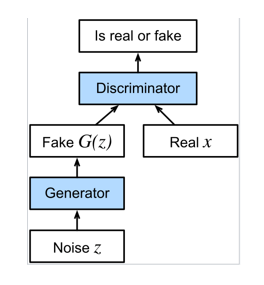
\includegraphics[width=0.5\textwidth]{Imgs/GAN_General_Arch.png}
    \caption{GAN General Architecture}
    \label{fig:GAN_Arch}
\end{figure}



\subsubsection{\ac{SDA}} \ac{SDA} is a deep neural network architecture designed for unsupervised feature learning and robust data representation\cite{vincent2010sda}. It is constructed by stacking multiple denoising autoencoders on top of each other, where each autoencoder layer is trained to reconstruct its input from a corrupted version of it. The key idea behind an \ac{SDA} is to intentionally introduce noise into the input data and force the network to learn a compressed representation that captures the underlying structure of the data rather than memorizing it. Each individual denoising autoencoder consists of an encoder function that maps the input vector to a latent representation and a decoder function that attempts to reconstruct the original clean input. After training one layer, its encoded output is used as the input to the next layer, allowing the network to progressively learn higher-level and more abstract features. This layer-wise training strategy improves convergence and helps mitigate issues such as vanishing gradients in deeper architectures. In anomaly detection scenarios, such as in \ac{ICS}, a \ac{SDA} is typically trained only on benign (normal) data so that it learns a faithful representation of normal system behavior.

\section{Provided Datasets}

For our project we were presented with two different datasets.
Electra\footnote{\url{http://perception.inf.um.es/ICS-datasets/csv/electra_s7comm.zip}} and 2017QUTS7Comm \footnote{ \url{https://github.com/qut-infosec/2017QUT_S7comm}} 
The Electra S7Comm dataset and the 2017QUTS7Comm dataset differ substantially in origin, structure, and format. Electra S7Comm was published by the University of Murcia (Spain) and was collected from realistic industrial testbeds~\cite{electra}. In contrast, 2017QUTS7Comm was generated in a controlled laboratory environment by the Queensland University of Technology~\cite{acisp2017}.



\subsection{Statistical Characteristics}
The Electra S7Comm dataset comprises approximately 387 million packets,
with roughly two thirds benign traffic and one third attack traffic.
All packets belong to the S7Comm protocol over \ac{TCP}.
Communication is limited to four host pairs, consisting of two benign
communication pairs and two attack-related pairs.

The 2017QUTS7Comm dataset contains approximately 10.8 million packets
and exhibits a strong class imbalance toward attack traffic.
While S7Comm constitutes the majority of traffic, additional
application-layer protocols such as \ac{NTP}, DHCPv6, \ac{NBNS}, and \ac{mDNS} are present.
Both \ac{TCP} and \ac{UDP} transport protocols occur in the dataset.

In total, 26 distinct host communication pairs are observed in
2017QUTS7Comm. However, the attack traffic is generated from a limited
set of attacker endpoints, with attack activity primarily originating
from a single source IP address interacting with different targets.

	\chapter{Our Approach}
\label{chap:approach}

In this chapter, we present our approach for processing the dataset and performing reverse engineering of the network packets. These steps are essential to transform raw proprietary \ac{ICS} traffic into a structured representation that can be used for anomaly detection without relying on protocol specifications. We further describe the construction of the different \ac{RE} datasets. This process is particular important, as it allows us to isolate and emphasize the physical readings that are most likely related to the underlying industrial process, thereby reducing the noise introduced by protocol-related bytes. Finally, we outline the implementation of the various detection methods, which are subsequently used as anomaly detection models. The comparison of these methods enables us to evaluate how effectively the extracted representations support the identification of abnormal behavior in \ac{ICS} environments.\footnote{You can find all implementations in our  repository on github: \url{https://github.com/abdelazizSalah/Study_Project}.}



\section{Procedure Overview}

Given that our research objective involves the investigation of reverse-engineering approaches, access to raw network packets was required. As the Electra dataset does not provide such data, the QUTS7Comm dataset was selected for all subsequent experiments.

The following section presents an overview of the complete processing and evaluation pipeline employed in this study project.

\begin{figure}[htb]
	\centering
	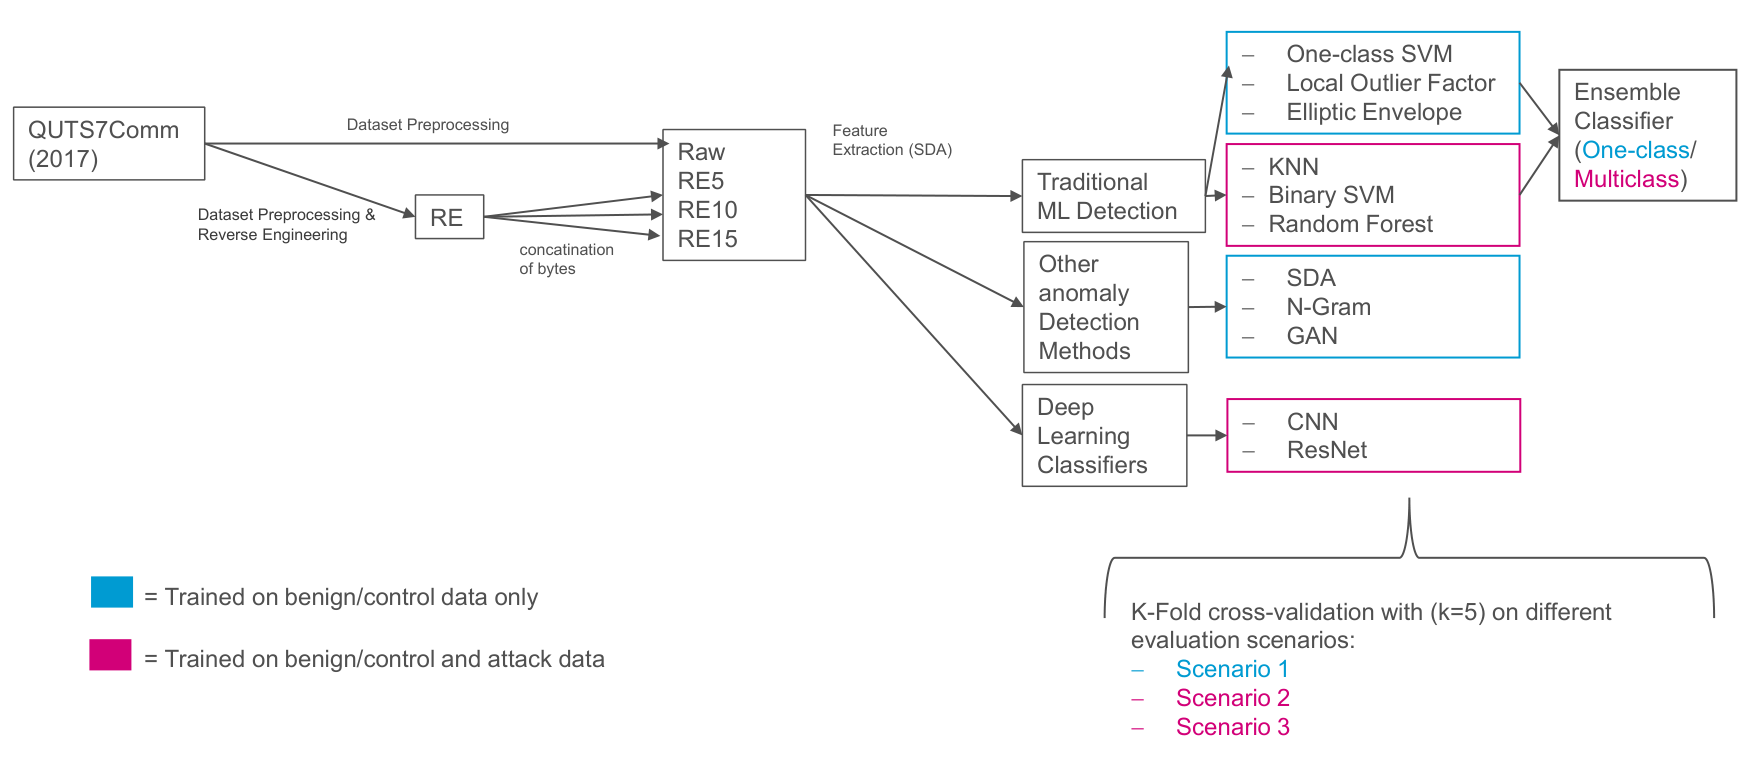
\includegraphics[width=\linewidth]{chapters/overview.png}
	\caption{Overview of proposed processing and evaluation pipeline}
 \label{fig:ourProcess}
\end{figure}

\Cref{fig:ourProcess} presents the complete processing pipeline of our
approach. The workflow begins with the provided \ac{pcap} files from the
2017QUTS7comm dataset. These packet captures are transformed and
preprocessed using two alternative strategies.

The first strategy operates directly on the raw packet data
(\textit{RAW} representation). The second strategy applies a
reverse-engineering procedure to extract a dynamic payload region,
which is assumed to contain process-related information.
After extraction, consecutive payload segments are concatenated
according to a parameter $p$, which controls the number of packets
aggregated into a single sample.

As a result, four dataset representations are generated:
\begin{itemize}
    \item \textbf{RAW}: processed packet data without reverse engineering,
    \item \textbf{RE5}, \textbf{RE10}, and \textbf{RE15}: reverse-engineered
    representations using $p \in \{5,10,15\}$, respectively.
\end{itemize}

Next, a \ac{SDA} is used to extract a compact latent feature vector
from each representation. These feature vectors serve as input for
the traditional \ac{ML} and selected \ac{DL} models.

The detection problem is considered from two perspectives:
outlier detection and supervised classification.
Accordingly, both one-class and supervised classifiers are evaluated.

We employ six traditional \ac{ML} models:

\begin{itemize}
    \item \textbf{One-class models:}
    \begin{itemize}
        \item One-Class \ac{SVM}
        \item \ac{LOF}
        \item \ac{EE}
    \end{itemize}
    
    \item \textbf{Supervised models:}
    \begin{itemize}
        \item Binary \ac{SVM}
        \item \ac{KNN}
        \item Random Forest
    \end{itemize}
\end{itemize}

In addition, two \ac{DL} classifiers are investigated:

\begin{itemize}
    \item \ac{CNN}
    \item \ac{ResNet}
\end{itemize}

Finally, three additional anomaly detection approaches are evaluated:

\begin{itemize}
    \item Reconstruction-error-based \ac{SDA}
    \item N-gram model
    \item \ac{GANs}-based detection
\end{itemize}

All detection methods are evaluated under three predefined
evaluation scenarios using $k$-fold cross-validation.

%%{\color{red} Due to limitation of our dataset size,} we needed to perform k-folding, however we considered performing the k-folding with three different scenarios. And for our whole experiments we considered the value of k to be equal to 5.  



\section{Dataset Pre-processing}

During the preprocessing we transform the provided PCAP files into
structured datasets suitable for training and evaluating the detection
methods. The process consists of label extraction, metadata parsing,
and the construction of two different dataset representations: RAW
and \ac{RE}.

%labe extraction
Attack labels were derived from the dataset folder structure.
Each PCAP file corresponds to either benign traffic or a specific
attack type, which allows assigning ground-truth labels to all
contained packets.
For every packet, we extracted relevant metadata including timestamps,
source and destination \ac{IP} addresses, and source and destination
port numbers. This metadata was used for filtering and dataset
organization but was not directly provided as input to the detection
models.

%raw ds representation

For the RAW representation, all packets contained in the PCAP files
were included without protocol-level filtering. This includes packets
without application-layer payload as well as packets unrelated to
the S7 communication protocol.

Each packet was represented by its complete raw byte sequence,
including Ethernet, \ac{IP}, and \ac{TCP}/\ac{UDP} headers followed by the
application-layer payload (if present). No additional parsing or
content truncation was performed in this representation.

%re dataset representaion

For the \ac{RE} representation, only S7Comm-related
application-layer data was considered. Packets were filtered according
to the following criteria:

\begin{itemize}
    \item The packet contains a \ac{TCP} layer,
    \item Either the source or destination port equals 102 (standard S7Comm port),
    \item The packet length satisfies the minimum structural size of
          TPKT (4 bytes), COTP (3 bytes), and S7 header (12 bytes).
\end{itemize}

After identifying valid S7Comm packets, only the application-layer
payload was retained. Based on the keyword position determined during
the reverse engineering phase, the byte sequence was truncated such
that only the payload starting from the identified keyword was used.
The keyword is identified in the Reverse Engineering process, as we describe in the following \cref{sec:rev-eng}. 
This representation therefore focuses on protocol-relevant content
rather than the full packet structure.

\subsection{Concatenation of Bytes to create RE5,RE10,RE15}

After identifying the index of the most suitable candidate keyword, we focused on extracting only the physical reading from the packets. However, we observed that extracting the physical reading from each packet individually results in very short byte sequences, which may not provide sufficient information for effective analysis. 

To address this limitation, we introduced a parameter denoted as \textit{p}, which defines the number of consecutive packets to be combined together. As illustrated in figure \ref{fig:ConcatenationOfBytes}, we concatenate the physical readings - which are located directly after the index of the best candidate - of every p consecutive raw packets to construct a single sample in the \ac{RE} dataset. 

More specifically, the physical readings extracted from raw packets $p_1$, $p_2$, ..., $p_p$ are concatenated to form single \ac{RE} sample. This process is repeated sequentially over the entire raw dataset. If the total number of raw packets is not divisible by p, the remaining packets at the end of the dataset are concatenated together without further padding or duplication. This concatenation strategy enables us to achieve three main objectives. First, it allows us to focus exclusively on the physical readings as features, thereby eliminating irrelevant protocol-related bytes from the analysis. Second, by combining consecutive packets, we partially reconstruct the contextual and temporal relationship between physical readings, which may improve the representational quality of the data. Finally, it allows us to systematically evaluate the impact of varying the parameter \textit{p} on the performance of the different detection methods. 



\begin{figure}[h]
    \centering
    \includesvg[width=0.8\textwidth]{Imgs/Concatenation}
    \caption{Concatenation of Bytes}
    \label{fig:ConcatenationOfBytes}
\end{figure}



\section{Reverse engineering}
\label{sec:rev-eng}
The objective of the reverse engineering process is to identify the
byte position (keyword) after which physical process readings are most
likely contained within the S7 communication payload. Since the protocol
specification is not explicitly parsed, the goal is to infer structural
patterns directly from the observed traffic.

\subsection{Identifying Keyword Candidates}

Firstly we identify all possible keyword candidates, by applying the following processing steps on the network traffic packets from the raw pcap files. 

\textbf{Session Extraction}

The network traffic is divided into communication sessions.
Sessions are identified based on the tuple
(source \ac{IP}, destination \ac{IP}, source port, destination port)
combined with a time window derived from packet inter-arrival times.
This grouping separates independent communication instances and
also distinguishes between client-to-server and server-to-client
directions.

\textbf{Progressive Sequence Alignment}

For each session and communication direction, progressive sequence
alignment is performed over all communication sessions. The purpose of
this alignment is to identify recurring structural patterns across
multiple messages.

\textbf{Identification of Static and Dynamic Fields}

Based on the aligned sequences, byte positions are classified as
\emph{static} if they remain constant across messages and as
\emph{dynamic} if their values vary.

Static byte positions typically correspond to protocol headers,
control fields, or structural identifiers, while dynamic positions
are potential candidates for variable data such as physical readings.
Adjacent static byte positions are merged into static fields to
form coherent structural blocks.

\textbf{Clustering of Dynamic Fields}

After separating static and dynamic fields, each dynamic field is
considered as a potential keyword candidate. For each candidate,
the subsequent payload region (i.e., the remaining frame behind the
candidate position) is extracted and grouped into value-based clusters.
The clustering is performed by grouping aligned
messages according to the byte values of the candidate field: messages with identical values
in the candidate interval $[start,end]$ are assigned to the same cluster.

The intuition is that if a candidate position marks the beginning
of physical readings, the subsequent byte sequences should exhibit
consistent value patterns across similar operational states.

\subsection{Cluster-Similarity Analysis for Keyword Selection}


After generating value-based clusters for each keyword candidate field, we analyze the
resulting cluster structure to identify the best keyword candidate.
For this we used the following approaches.
 

\subsubsection{Payload-Length Homogeneity within Clusters}
In addition to cluster-size statistics, we analyze whether messages grouped by a keyword
candidate exhibit consistent payload characteristics. For each aligned message, we compute its
effective payload length as the number of non-empty bytes (non-\texttt{None} positions) in the
alignment. For each cluster with at least two messages, we compute the standard deviation of
these payload lengths and aggregate the values across clusters using a size-weighted average.
A low homogeneity score indicates that messages within the same cluster have similar payload
lengths, which is expected when the candidate field groups messages into structurally similar
types. Candidates achieving low within-cluster variability are therefore considered more likely
to mark a meaningful boundary in the protocol payload.
\subsubsection{Joint Probability}

Not every candidate keyword identified during the previous steps represents a valid protocol keyword. Therefore, we introduce several constraints in order to filter out unlikely candidates. 

First, we define a maximum keyword length constraint. This constraint introduces a parameter \textit{L}, which represents the maximum allowed length of a keyword. Length of a keyword is defined as the number of bytes in the keyword. Any candidate keyword whose length exceeds \textit{L} is discarded. This step reduces the number of potential candidates and removes fields that are unlikely to represent protocol keywords.

For the remaining candidates, we evaluate the quality of the clustering results by computing three probability measures. These probabilities assess different structural and behavioral properties of the clusters and help determine the most likely keyword candidate.

\begin{itemize}

\item \textbf{Message Similarity ($P_m$):}  
This probability measures the similarity between messages within and across clusters. The underlying assumption is that messages belonging to the same cluster should exhibit higher similarity than messages belonging to different clusters.

For every pair of messages, we compute a similarity score defined as the ratio between the number of identical bytes and the total number of bytes in both messages. These scores form a similarity matrix containing the similarity values for all message pairs.

Based on the clustering results for a given keyword candidate, the similarity scores are divided into two groups:
\begin{itemize}
\item \textit{Intra-scores}: similarity scores between messages belonging to the same cluster.
\item \textit{Inter-scores}: similarity scores between messages belonging to different clusters.
\end{itemize}

A threshold parameter \textit{T} is then introduced in order to compute two additional metrics:

\begin{itemize}
\item \ac{FMR}:
\[
FMR = \frac{\#(\text{inter-scores} > T)}{\text{total number of inter-scores}}
\]

\item \ac{FNMR}:
\[
FNMR = \frac{\#(\text{intra-scores} < T)}{\text{total number of intra-scores}}
\]
\end{itemize}

Using these values, the message similarity probability is defined as:

\[
P_m = 1 - \frac{FMR + FNMR}{2}
\]

A higher value of $P_m$ indicates that the candidate keyword produces clusters with high internal similarity and low similarity across clusters, which suggests a good keyword candidate.

\item \textbf{Remote Coupling ($P_r$):}  
This probability evaluates the relationship between clusters of client messages and clusters of server responses. The intuition behind this metric is that messages of the same type sent by a client should typically trigger similar responses from the server.

The computation proceeds as follows:

\begin{enumerate}
\item Client-to-server messages are clustered.
\item Server-to-client messages are clustered independently.
\item Messages are then paired according to their TCP session order.
\end{enumerate}

For each client cluster we define:
\begin{itemize}
\item $N$: the number of client messages in the cluster.
\item $M$: the largest number of corresponding server responses that belong to the same server cluster.
\end{itemize}

The remote coupling probability is then defined as:

\[
P_r = \frac{M}{N}
\]

A high value of $P_r$ indicates strong correspondence between client requests and server responses, suggesting that the candidate keyword correctly separates different message types.

\item \textbf{Structure Coherence ($P_s$):}  
This probability measures how consistent the internal structure of messages is within each cluster. The assumption is that messages of the same type should share a similar structural format.

For each cluster, the messages are aligned again and the number of alignment gaps introduced during this process is counted. The probability is then computed as:

\[
P_s = 1 - \frac{\text{average number of gaps}}{\text{aligned message length}}
\]

A higher value of $P_s$ indicates that messages within the cluster share a consistent structure, which supports the validity of the candidate keyword.

\end{itemize}

Finally, we compute the joint probability as

\[
P_t = P_m \cdot P_r \cdot P_s
\]

under the assumption that the three probabilities are independent. The resulting value represents the overall likelihood that a candidate field corresponds to a valid protocol keyword. Candidates with higher values of $P_t$ are therefore considered more likely to represent legitimate keywords. And best keyword should be teh one with the highest joint probability.

Following this scheme we managed to correctly detect the best keyword in protocol S7comm, and we identified the keyword index 12 as shown in figure \ref{fig:best_Candidate_S7comm}, which is \textit{Item count field}, after which we can find the physical readings.
\begin{figure}[htb]
	\centering
	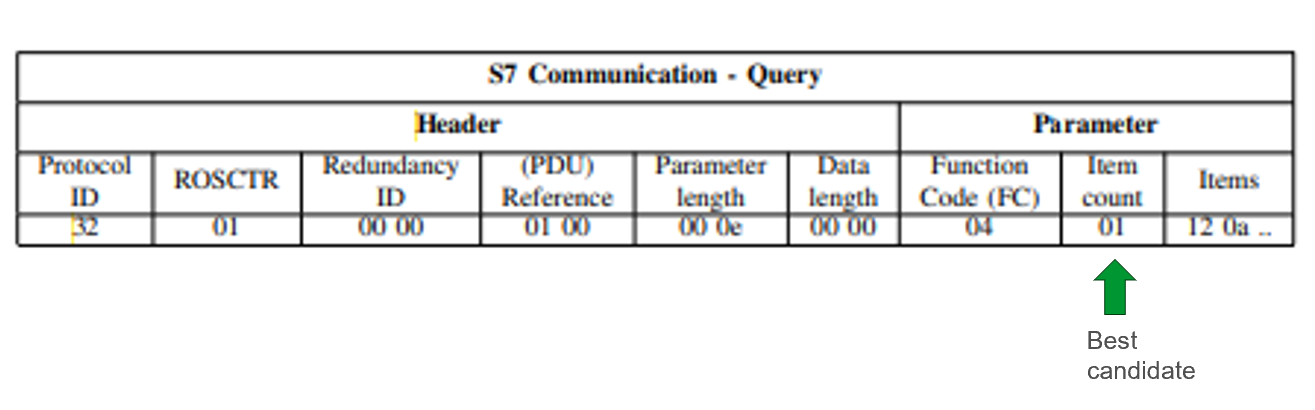
\includegraphics[width=\linewidth]{Imgs/S7comm_Best_Candidate.png}
    \caption{Determining best candidate index in S7comm protocol}
    \label{fig:best_Candidate_S7comm}
\end{figure}

\section{Evaluation Strategy}
To ensure a fair and systematic comparison of the implemented
detection methods, a structured evaluation strategy is adopted.
\subsection{Implementation of Evaluation Scenarios with K-Fold Cross-Validation}

Three evaluation scenarios are defined to simulate
different training conditions, ranging from purely benign
training data to partially supervised settings with varying
numbers of attack types.

\begin{itemize}
\item \textbf{Scenario 1:} The training set contains only benign samples.
\item \textbf{Scenario 2:} The training set contains all benign samples and
samples from $N-2$ of the $N$ attack types.
\item \textbf{Scenario 3:} The training set contains all benign samples and
samples from one randomly selected attack type.
\end{itemize}

In all scenarios, the test set contains benign samples as well as
samples from all attack types.

All scenarios are implemented using $k$-fold cross-validation with 5 iterations (k=5).

This method is used to obtain robust performance estimates by evaluating each model on multiple train-test splits. In addition, cross-validation makes efficient use of the available data, since every sample is used for validation exactly once and for training in the remaining folds.


\begin{figure}[htb]
	\centering
	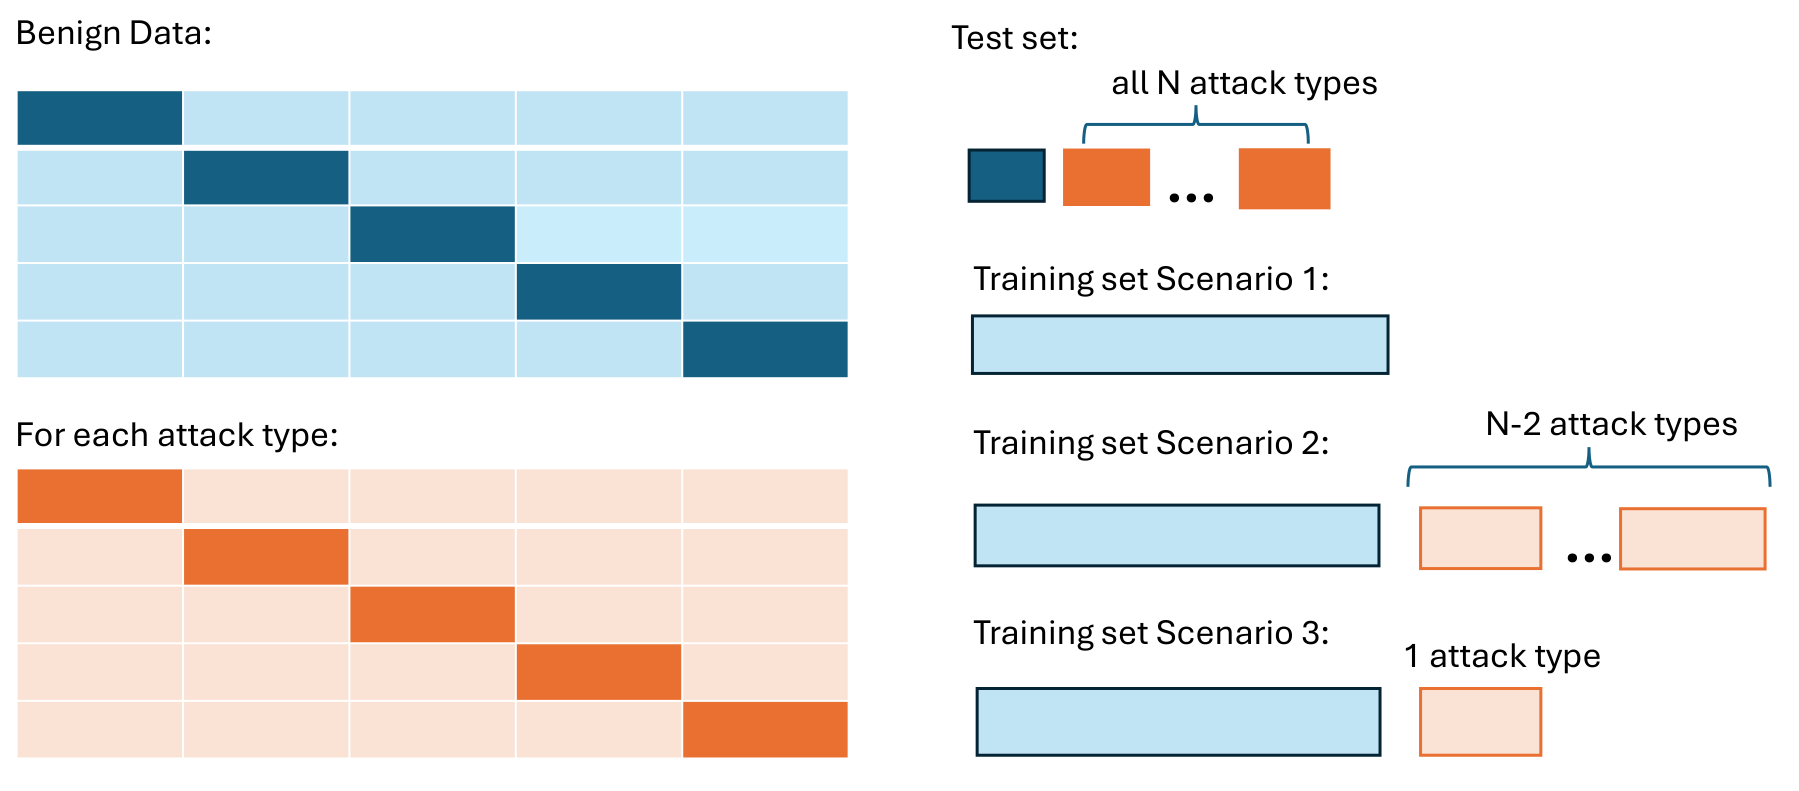
\includegraphics[width=\linewidth]{chapters/k_folds.png}
	\caption{K-Fold cross-validation adapted to the three evaluation scenarios}
	\label{fig:kfolds}
\end{figure}

To integrate the evaluation scenarios into the cross-validation
procedure, the dataset is first partitioned into benign samples
and separate subsets for each attack type.
Cross-validation is then performed independently on each subset.

As illustrated in figure \ref{fig:kfolds}, in each iteration the validation
fold of the benign subset is combined with the corresponding
validation fold of each attack-type subset to form the test split.
Consequently, the test split remains identical across all scenarios,
ensuring comparability between them.

The training split differs depending on the scenario:
\begin{itemize}
\item In \textbf{Scenario 1}, only the $k-1$ benign training folds are used.
\item In \textbf{Scenario 2}, the benign training folds are combined
with the $k-1$ training folds of $N-2$ attack types.
\item In \textbf{Scenario 3}, the benign training folds are combined
with the $k-1$ training folds of one randomly selected attack type.
\end{itemize}

As a result, the benign portion of the training data remains identical
across scenarios, while only the included attack types vary.
This design ensures that performance differences between scenarios
can be attributed to changes in attack diversity rather than
differences in test data.

\subsection{Evaluation Methods}

For each implemented model, hyperparameter tuning is performed
to determine optimal parameter configurations. It was usually performed using grid-search approach using the standard recommended values for each parameter.
Subsequently, experiments are conducted using these optimized
parameters within each fold and evaluation scenario.
Performance metrics are averaged across all cross-validation runs.

Since the test sets in all scenarios contain both benign and
attack samples and are not class-balanced, accuracy is not used
as the primary evaluation metric.
Instead, we report the F1-score,
which provides a more informative assessment under skewed
class distributions.

Beyond overall detection performance, we additionally analyze
feature importance, error overlaps, and computational complexity
(runtime and memory consumption) for the traditional ML classifiers.
These analyses are conducted for the RAW dataset representation
and for the RE15 representation to enable a detailed comparison
of classifier behavior under full and reduced feature sets.
%Feature Importance
\subsubsection{Feature Importance Analysis}
\label{subsubsec:feature_importance}

To better understand the contribution of the extracted features to the classification
decision, we perform a feature importance analysis for the traditional machine learning
classifiers. Since different models provide different interpretability mechanisms,
model-specific importance measures are used.

For the binary linear \ac{SVM}, feature importance is computed
as the absolute magnitude of the learned weight vector, i.e., $|\mathbf{w}|$,
which reflects the contribution strength of each input feature to the decision boundary.

For the Random Forest classifier, we use the built-in impurity-based importance
measure (mean decrease in impurity), which quantifies how much each feature
contributes to reducing node impurity across all trees in the ensemble.

For all other traditional \ac{ML} classifiers, permutation-based feature importance
is applied. In this approach, the values of a single feature are randomly permuted,
and the decrease in model performance is measured. A larger performance drop
indicates higher feature relevance.

The resulting importance scores are normalized and ranked in descending order.
This analysis allows us to identify which autoencoder-generated features contribute
most to attack detection and to compare feature reliance across different models.

%Venn Diagrams for Error Overlaps
\subsubsection{Error Overlap Analysis}

To analyze the overlap of classification errors among different detection methods,
we construct Venn diagrams for each evaluation scenario. Each circle represents the set
of misclassified test samples produced by a particular classifier. Intersections between
circles indicate samples that were misclassified by multiple models simultaneously.

This analysis provides insight into whether different classifiers fail on the same
instances or whether their errors are complementary. A high degree of overlap suggests
that the models capture similar patterns, whereas low overlap indicates complementary
behavior.

%Runtime and Memory consumtion
\subsubsection{Runtime and Memory Consumption}

In addition to detection performance, we evaluate the computational complexity of
each method in terms of runtime and memory consumption. For each model, we measure:

\begin{itemize}
    \item Feature generation time, measured separately for (i) training the autoencoder and (ii) extracting features from the trained model
    \item Average training time and average inference time for each traditional \ac{ML} detection method,
    \item Peak memory usage during feature generation,  measured separately for (i) training the autoencoder and (ii) extracting features from the trained model
    \item Peak memory usage during training and inference for each traditional ML detection method.
\end{itemize}

Runtime is measured using system time functions, while memory consumption is monitored
using profiling tools. The reported values correspond to the average across all
cross-validation folds.

This analysis allows us to compare the practical feasibility of traditional machine
learning methods.

\section{Implementation of Anomaly detection methods}

This subsection describes the traditional machine learning methods used for anomaly detection. 
First, we explain how latent features are extracted from the packet data using the \ac{SDA}. These features are then used as input to our classifiers implemented in our framework.

\subsection{Traditional \ac{ML} detection methods}


To apply traditional machine learning classifiers to network packet data, a fixed-length feature 
representation is required. Therefore, we first extract compact latent representations from the 
raw packet data using the \ac{SDA}.


%ToDo Anna
\subsubsection{Feature Extraction using the \ac{SDA}}
Traditional ML classifiers such as \ac{SVM}, \ac{KNN}, and Random Forest require a fixed-length, low-dimensional feature representation and do not natively handle variable-length byte sequences. Therefore we employ a \ac{SDA} as a feature extractor to obtain compact latent representations of the preprocessed
packet data. These latent feature vectors are subsequently used as input to all traditional
machine learning detection methods.

Each sample in a dataset representation (RAW, RE5, RE10, RE15) is given as a byte-vector.
To ensure a fixed input dimensionality, every byte-vector is either truncated or zero-padded
to a predefined length $M$ and then normalized to the range $[0,1]$. In our experiments,
$M$ was set to the length of the longest packet (or concatenated RE sequence) within the
corresponding representation.
For each dataset representation, the \ac{SDA} is trained exclusively on benign samples and on the training set from the current k-fold iteration. Using only benign samples enables the
model to learn a compressed representation of normal traffic patterns.

After training, the \ac{SDA} is used to encode all samples of the corresponding representation.
Concretely, each input byte-vector is forwarded through the encoder, and the output vector of
the bottleneck layer are extracted as the latent feature vector. In our implementation, the
bottleneck produces a 32-dimensional feature vector per input sample, resulting in a compact
representation that is used for subsequent training and evaluation of the traditional ML
classifiers.

\subsubsection{Ensemble Classifier Implementation}

\begin{figure}[htb]
	\centering
	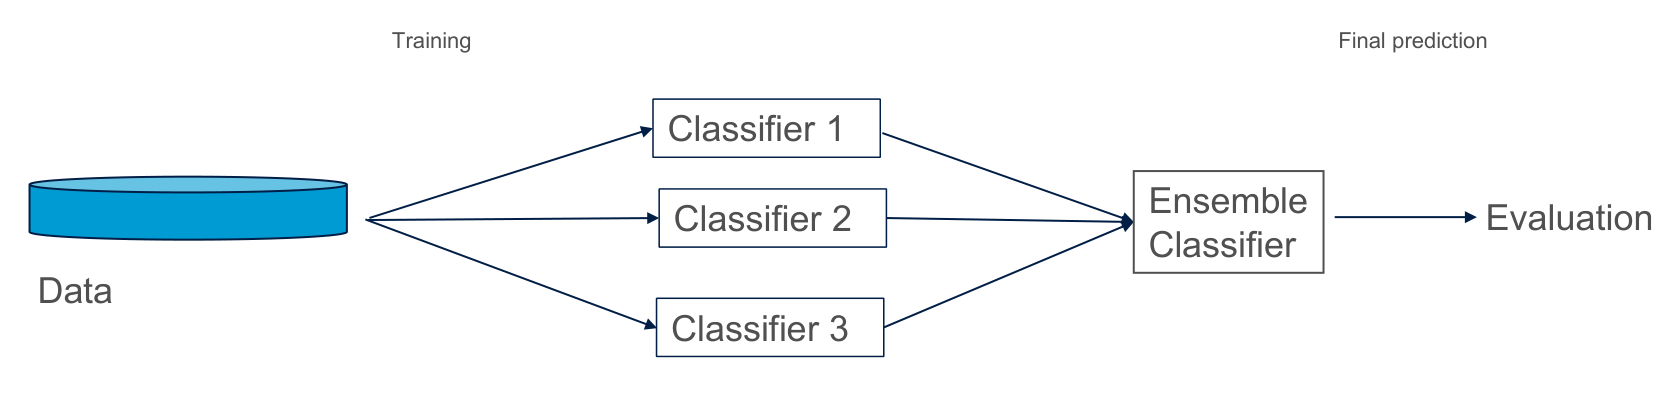
\includegraphics[width=\linewidth]{chapters/ensembleClassifier.png}
	\caption{Ensemble Classifier Structure}
 	\label{fig:ensemble-structure}
\end{figure}
In order to reduce model-specific errors and leverage complementary strengths to achieve an overall more robust and stable detection performance we combine the traditional ML classifiers into an ensemble classifier. 

As illustrated in figure \ref{fig:ensemble-structure} the ensemble classifier combines the predictions of three independently
trained traditional machine learning models.
 Each base classifier is
trained separately using the corresponding training split of the
cross-validation procedure. During inference, all three classifiers
produce an individual prediction for each test instance.

The final decision of the ensemble is obtained by aggregating the
three individual predictions according to a predefined aggregation
strategy. In our implementation, the following prediction modes are
supported:

\begin{itemize}
    \item \textbf{Random:} One of the three predictions is selected uniformly at random.
    \item \textbf{Majority:} The final prediction corresponds to the class predicted by the majority of the three classifiers.
    \item \textbf{All:} A sample is classified as an attack only if all three classifiers predict it as an attack; otherwise, it is classified as benign.
\end{itemize}

Since the project includes six traditional ML detection methods: three
operating as one-class (outlier) detectors and three operating as
binary classifiers—we implemented two operational ensemble modes:

\begin{itemize}
    \item \textbf{One-Class Mode:} The ensemble aggregates the predictions of the three outlier detectors (One-Class SVM, LOF, and Elliptic Envelope).
    \item \textbf{Binary Classification Mode:} The ensemble aggregates the predictions of the three binary classifiers (Binary SVM, k-Nearest Neighbors, and Random Forest).
\end{itemize}

\subsection{\ac{DL} detection methods}


In addition to traditional machine learning approaches, we implement deep learning based
detection methods that can learn hierarchical feature representations directly from the
raw byte sequences of network packets. Unlike traditional classifiers, deep neural networks
can automatically capture complex spatial patterns and dependencies in packet data without
relying on manually engineered features.

In particular, we investigate \ac{CNN} and \ac{ResNet}. \ac{CNN}s are well suited for analyzing structured sequential data such as byte
sequences, as convolutional filters can learn local patterns that frequently occur in
network packets. \ac{ResNet} extends this idea by introducing residual connections that allow
training deeper neural architectures while mitigating the vanishing gradient problem.
These models enable the system to learn more expressive representations of the packet
structure and improve anomaly detection performance.

\subsubsection{\ac{CNN}}
%ToDo Anna

We implemented a \ac{CNN} to perform binary attack detection directly on the preprocessed byte sequences (i.e., without using the autoencoder-generated features). Similar to the feature generation pipeline, all
inputs are converted to a fixed length of $M$ bytes by truncation or zero-padding to ensure a
consistent input shape. For our experiments, $M$ was set to the length of the longest packet
in the corresponding dataset representation. Each sample is provided to the network in the
shape $(M,1)$, where the last dimension represents the single input channel.

The CNN consists of four convolutional blocks followed by a dense classification head.
Each convolutional block contains two repetitions of the sequence
\emph{Conv1D $\rightarrow$ Batch Normalization $\rightarrow$ Activation $\rightarrow$ Dropout}.
The convolution layers learn local byte-patterns by applying trainable filters across the input
sequence, batch normalization stabilizes training by normalizing intermediate activations, and
dropout reduces overfitting by randomly deactivating a fraction of units during training.
The number of filters increases with network depth (e.g., $8,16,32,64$), enabling the model to
learn progressively more abstract representations.

To reduce the temporal resolution between blocks, we apply downsampling either via
MaxPooling1D after each block or by using stride-2 in the first convolution of blocks two to
four (depending on the selected configuration). After the fourth block, the resulting feature
maps are transformed into a fixed-size vector using a global pooling operation.
By default, we apply Global Average Pooling, which aggregates each feature map by averaging
over its length dimension and produces a compact representation for the dense layers.

Finally, the network applies a fully connected layer (with batch normalization, activation, and
dropout) and a Softmax output layer with two neurons to predict the probability of the classes
\emph{benign} and \emph{attack}. The model is optimized using Adam and categorical cross-entropy
loss. Architecture-related hyperparameters (e.g., activation function, kernel size, dropout rate,
downsampling strategy, and pooling type) as well as optimization parameters were selected via
grid search on the training split.

\subsubsection{\ac{ResNet}} 
 In the context of anomaly detection in \ac{ICS}, ResNet can be adapted to process one-dimensional byte sequences of network packets using one-dimensional convolutional layers. The residual connections help preserve low-level structural information while progressively extracting higher-level representations, which improves classification performance on complex and high-dimensional network traffic data. Due to its stable training behavior and strong representational capacity, ResNet is particularly suitable for modeling subtle deviations in proprietary binary communication protocols. ResNet accepts as an input \textit{m} x \textit{n} complete network packets or the parsed physical readings, where m is the number of packets, and n is the number of bytes per each packet. 


\begin{figure}[h]
    \centering
    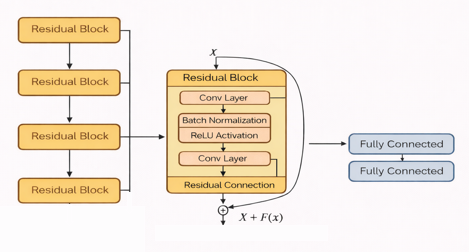
\includegraphics[width=1.0\textwidth]{Imgs/ResNetArch.jpg}
    \caption{ResNet18 Architecture}
    \label{fig:resNetArch}
\end{figure}

\vspace{10px}


\paragraph{Our implementation} We managed to implement ResNet18 which contains of 18 layers in total.  these layers are divided into four main residual blocks as shown in figure \ref{fig:resNetArch} and each block consists of two convolution blocks. Each convolution block contains two convolution layers with a batch normalzation and ReLU non-linear activation function in between. After the 4 residual blocks, we forward the output to two fully-connected layers, that will use the reduced data to classify the network packet using sigmoid function. We used Adam optimizer to update weights, and for the loss function we used categorical cross-entropy. 
\paragraph{Statistical features} Along with the raw network packets, and the reverse engineered packets, we managed to extract 5 other statistical features and append them to the ResNet. 

\begin{enumerate}
    \item Total number of bytes in a given sample packet which is counted before trimming or padding this packet.
 \item Number of occurrence of the most often found byte
 \item Number of occurrence of the second most often found byte,
 \item Byte entropy, which measures randomness of packet bytes. It is computed as \[
E(P) = - \sum_{b=0}^{255} p(b)\,\log_2 p(b)
\] 
where $p(b)$ denotes the probability of observing byte value $b$ in the packet.
\[
p(b) = \frac{n_b}{N}
\]
where ${n_b}$ is number of  occurrences of byte b in the given packet, and N is the size of the packet. 
 \item \ac{RPB}, which tells the model how much of the input is artificial. It is computed as \[
\mathrm{RPB} = \frac{\text{number of bytes before padding}}{\text{total number of bytes}}
\]
\end{enumerate}

\subsection{Other anomaly detection methods}

In addition to the traditional ML and deep learning classifiers, we evaluate several alternative
approaches for anomaly detection. These include an SDA-based reconstruction error detector,
an n-gram statistical model that captures byte sequence patterns in network packets, and a
\ac{GANs} based method capable of modeling the distribution of
normal traffic. These methods provide complementary perspectives on anomaly detection by
leveraging reconstruction errors, statistical sequence modeling, and generative learning.

\begin{figure}[htb]
	\centering
	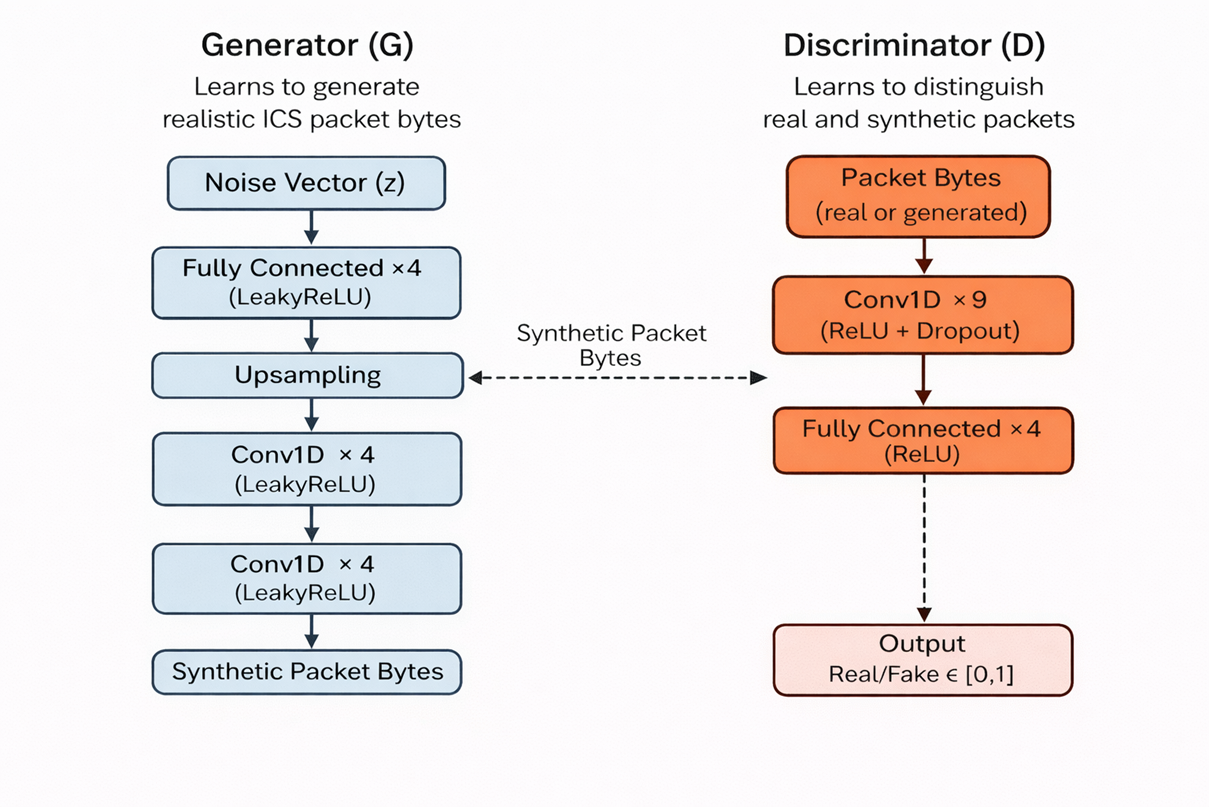
\includegraphics[width=\linewidth]{Imgs/Discriminator_and_Generator.png}
	\caption{Discriminator and Generator architectures}
    \label{fig:DandG}
\end{figure}


\subsubsection{\ac{SDA}-Based Reconstruction Error Detection}

The implemented \ac{SDA}
is employed as a standalone anomaly detection method based on
reconstruction error. The \ac{SDA} is trained exclusively on benign network traffic. During training,
the model learns a compressed latent representation of normal packets and
optimizes its parameters to minimize the reconstruction error between the
input and the reconstructed output. Since attack packets deviate from the
distribution of normal traffic, they are expected to be reconstructed less
accurately, resulting in a higher reconstruction error.

For a given input byte-vector $\mathbf{x} \in \mathbb{R}^M$, the trained
autoencoder produces a reconstruction $\hat{\mathbf{x}}$. The reconstruction
error is computed using the \ac{MSE}:

\begin{equation}
\text{MSE}(\mathbf{x}) = \frac{1}{M} \sum_{i=1}^{M} (x_i - \hat{x}_i)^2.
\end{equation}

To transform the \ac{SDA} into a binary classifier, a decision threshold
$\tau$ is defined based on the reconstruction error distribution of
benign training samples. Concretely, we compute the per-sample \ac{MSE}
for all benign training packets and set $\tau$ to the
$95^{\text{th}}$ percentile of these errors, i.e., such that
95\% of benign reconstruction errors lie below $\tau$.

During testing, each packet is processed by the trained \ac{SDA} and its
reconstruction error is computed. The final classification rule is:

\begin{equation}
\hat{y} =
\begin{cases}
\text{attack}, & \text{if } \text{MSE}(\mathbf{x}) > \tau, \\
\text{benign}, & \text{otherwise}.
\end{cases}
\end{equation}

Packets whose reconstruction error exceeds the predefined threshold
are therefore classified as anomalous.


\subsubsection{\ac{GANs}}
In anomaly detection scenarios, particularly in \ac{ICS}, GANs can be trained on normal data only, allowing the discriminator or generator to detect deviations from the learned distribution during testing. Because GANs are capable of learning complex, high-dimensional data distributions, they are well suited for modeling raw network packet bytes or other structured sequential inputs. 




\paragraph{Discriminator Implementation}
 
 Discriminator architecture as shown in figure \ref{fig:DandG} consists of \ac{CNN} that consists of 9 convolution layers with ReLU activation function, along with dropout layer after all convolution layers except the first and final layers. Output is passed to four fully connected layers with ReLU activation function, and the output is generated from Sigmoid function which predicts a value in range [0,1] indicating how fake the input data is, 0 means fake data, while 1 means real data. 

\paragraph{Generator Implementation} Generator is reverse \ac{CNN}. It uses \textit{deconvolution} operation, which is he inverse operation of convolution, which is a method to transform noise into meaningful network packets with a certain degree of accuracy. Its architecture as shown in figure \ref{fig:DandG}  consists of 4 fully connected layers with a LeakyReLU activation function, then they are followed by 8 convolution layers with LeakyReLU activation function. The first 4 layers from these 8 convolution layers are preceded by upsampling layers, the main reason for that is to increase the number of data samples in the dataset, which can helps in correcting imbalances in data, enhancing the quality of generated data, and improve the model performance.  We mainly used LeakyReLU here because we want to be able to regenerate the network packet out of noise input, so it can help us keeping as much neurons alive as possible to participate in the generation of the network packets. Moreover, for the generator we managed to implement custom loss function, which extract features from real and fake samples, and compute the mean feature vectors, then it computes L2 loss between mean feature vectors. \begin{lstlisting}
def feature_matching_loss(D, x_real, x_fake):
    '''
    Input:
        D: Discriminator model
        x_real: real data batch
        x_fake: fake data batch
    Output:
        loss: feature matching loss value
    '''
    f_real = D.extract_features(x_real)
    f_fake = D.extract_features(x_fake)

    mean_real = f_real.mean(dim=0)
    mean_fake = f_fake.mean(dim=0)

    loss = torch.mean((mean_real - mean_fake) ** 2) / mean_real.numel()
    return loss
\end{lstlisting}



\subsubsection{N-Gram} 
It is a contiguous sequence of $N$ items extracted from a larger sequence of data, where the items may represent characters, bytes, or tokens depending on the application domain. In the context of network traffic analysis, N-grams are typically constructed from raw packet bytes, meaning that each N-gram represents a sequence of $N$ consecutive bytes within a packet. N-gram is usually defined by 2 main parameters, the value of \textit{n}, which defines the number of consecutive bytes, and \textit{stride} which define the jumping value. For example a 2-gram (bigram) with stride = 1  captures pairs of adjacent bytes, while a 5-gram with stride = 1 captures sequences of five consecutive bytes. In figure \ref{fig:n-gram-example}, we demonstrate the idea of n-grams but on string of characters, when n=3, and stride=1, we can see that we consider the first three consecutive characters \textit{HEL} as one feature, then we increase the pointer position by the stride value which is equal to 1 in our case to next starting position, and it will be in our case letter \textit{E}, then we take 3 consecutive characters again to form \textit{ELL}, and we keep this process till the end of the string. On the second example you can see the stride value is 2, so it will have the same behavior, except that when we go to the next starting index, instead of increasing the starting position by 1, we will increase it by 2, so in the second iteration instead of starting from index 1, we will start from 2 which contains letter \textit{L} instead of letter \textit{E}.  The main idea behind N-gram modeling is that local sequential patterns contain meaningful structural information about the underlying data distribution. During the training phase, all distinct N-grams observed in benign traffic are collected and their frequencies are recorded, often using memory-efficient data structures such as \textbf{Bloom filters}. At testing time, a new packet is evaluated by measuring how many of its N-grams were previously observed during training and how frequently they occurred. We define a score for whether this packet is normal or malicious as: \[
\text{Score} = \frac{\sum_{i} w_i \cdot N_{\text{seen}_i}}{T}
\] 
$\text{Score} \in [0,1]$, where $N_{\text{seen}_i}$
indicates each n-gram in the packet that was seen during training,
wi represents its normalized weight how often this n-gram was seen during training, and T
represents the total number of n-grams in the current packet. Packets that contain a high proportion of unseen or rarely occurring N-grams are more likely to deviate from normal behavior and can therefore be classified as anomalous, in other words, packets with low scores should be classified as malicious. N-gram-based methods are particularly suitable for anomaly detection in \ac{ICS} because proprietary binary protocols often lack publicly available specifications, making direct parsing difficult. By operating directly on raw byte sequences without requiring protocol awareness, N-grams provide a simple yet effective statistical modeling technique for detecting deviations in structured network traffic. \paragraph{Bloom Filter} is a probabilistic data structure designed for efficient set membership testing with minimal memory consumption. It allows one to determine whether an element is possibly in a set or definitely not in a set. A Bloom filter consists of a fixed-size bit array and multiple independent hash functions. When inserting an element into the filter, the element is processed by each hash function, and the corresponding bit positions in the array are set to one. To check whether an element is present, the same hash functions are applied, and the bits at the resulting positions are inspected. If at least one of these bits is zero, the element is guaranteed not to be in the set. If all bits are one, the element is assumed to be in the set; however, this may result in a false positive due to hash collisions. Importantly, Bloom filters do not produce false negatives, meaning that an inserted element will never be reported as absent. The trade-off between memory usage and false positive probability depends on the size of the bit array and the number of hash functions used. In the context of N-gram-based anomaly detection for \ac{ICS}, Bloom filters are particularly useful for storing large numbers of observed N-grams in a space-efficient manner, enabling fast membership queries during testing without requiring storage of the full set of N-grams.

\begin{figure}[htb]
	\centering
	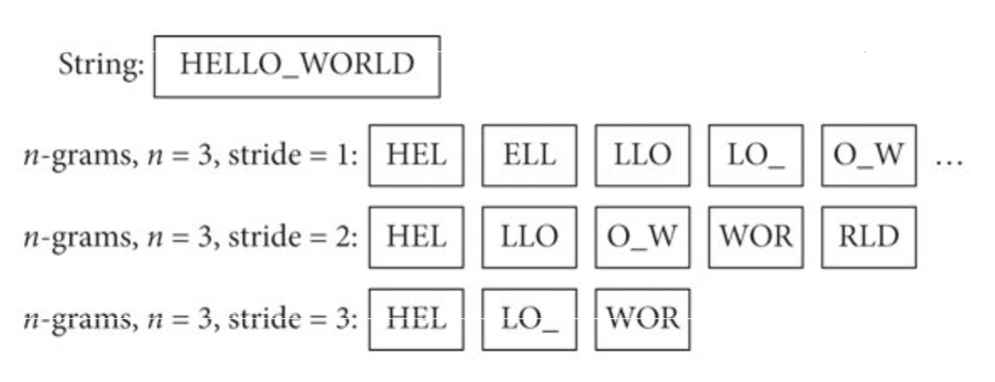
\includegraphics[width=\linewidth]{Imgs/n_grams_example.png}
	\caption{N-Gram Example}
	\label{fig:n-gram-example}
\end{figure}


\paragraph{Hash Functions and Double Hashing Strategy}


Instead of computing $k$ independent hash functions, we apply a double hashing strategy. 
Two base hash values $h_1(x)$ and $h_2(x)$ are computed, and the $i$-th hash value is generated as:

\[
h_i(x) = \left(h_1(x) + i \cdot h_2(x)\right) \bmod m
\]

where $m$ denotes the size of the Bloom filter in bits.

This approach significantly reduces computational cost while maintaining good distribution 
properties and minimizing correlations between generated hash values. For h1 and h2 we used both a non-cryptographic and a cryptographic hash function to ensure a good balance between speed and randomness, which are MurmurHash3 and BLAKE2b respectively.

\textbf{MurmurHash3} is a non-cryptographic hash function optimized for high speed and low computational overhead. 
It produces a uniform 64-bit output and is widely used in Bloom filters and hash tables due to its strong 
avalanche effect and low collision probability in practical applications.

\medskip

\textbf{BLAKE2b} is a cryptographic hash function designed to provide both high security and high performance. 
It generates outputs with strong entropy and collision resistance. 
In our implementation, we use an 8-byte (64-bit) digest to obtain a compact yet well-distributed hash value.



\begin{lstlisting}
def _hashes(self, data: bytes):
    '''
    Generate k hash values for the given data using double hashing.
    Parameters:
        data: byte sequence to be hashed

    Yields:
        k hash values in the range [0, m-1]
    '''

    # First hash: MurmurHash3 (fast, non-cryptographic)
    h1, _ = mmh3.hash64(data, seed=0, signed=False)

    # Second hash: BLAKE2b (cryptographic, strong entropy)
    blake = hashlib.blake2b(data, digest_size=8).digest()
    h2 = int.from_bytes(blake, "big") | 1  # ensure h2 is odd

    # Generate k hash values using double hashing
    for i in range(self.number_of_hash_functions):
        yield (h1 + i * h2) % self.required_number_of_bits
\end{lstlisting}



       \chapter{Evaluation}
\label{chap:evaluation}
In this chapter, we present the experimental results of the implemented detection methods. The evaluation is primarily based on tree performance metrics: precision, recall, and F1-score. By systematically comparing these metrics across the different methods, we are able to identify their respective strengths and limitations. This comparison further allows us to determine which approach achieves the best overall performance under the considered evaluation scenarios, as well as analyze the inherent trade-offs between detection accuracy and false positive or false negative rates. 

\section{Traditional \ac{ML} Detection Methods}
\subsection{F1-Scores}

\begin{figure}[!htbp]
	\centering
	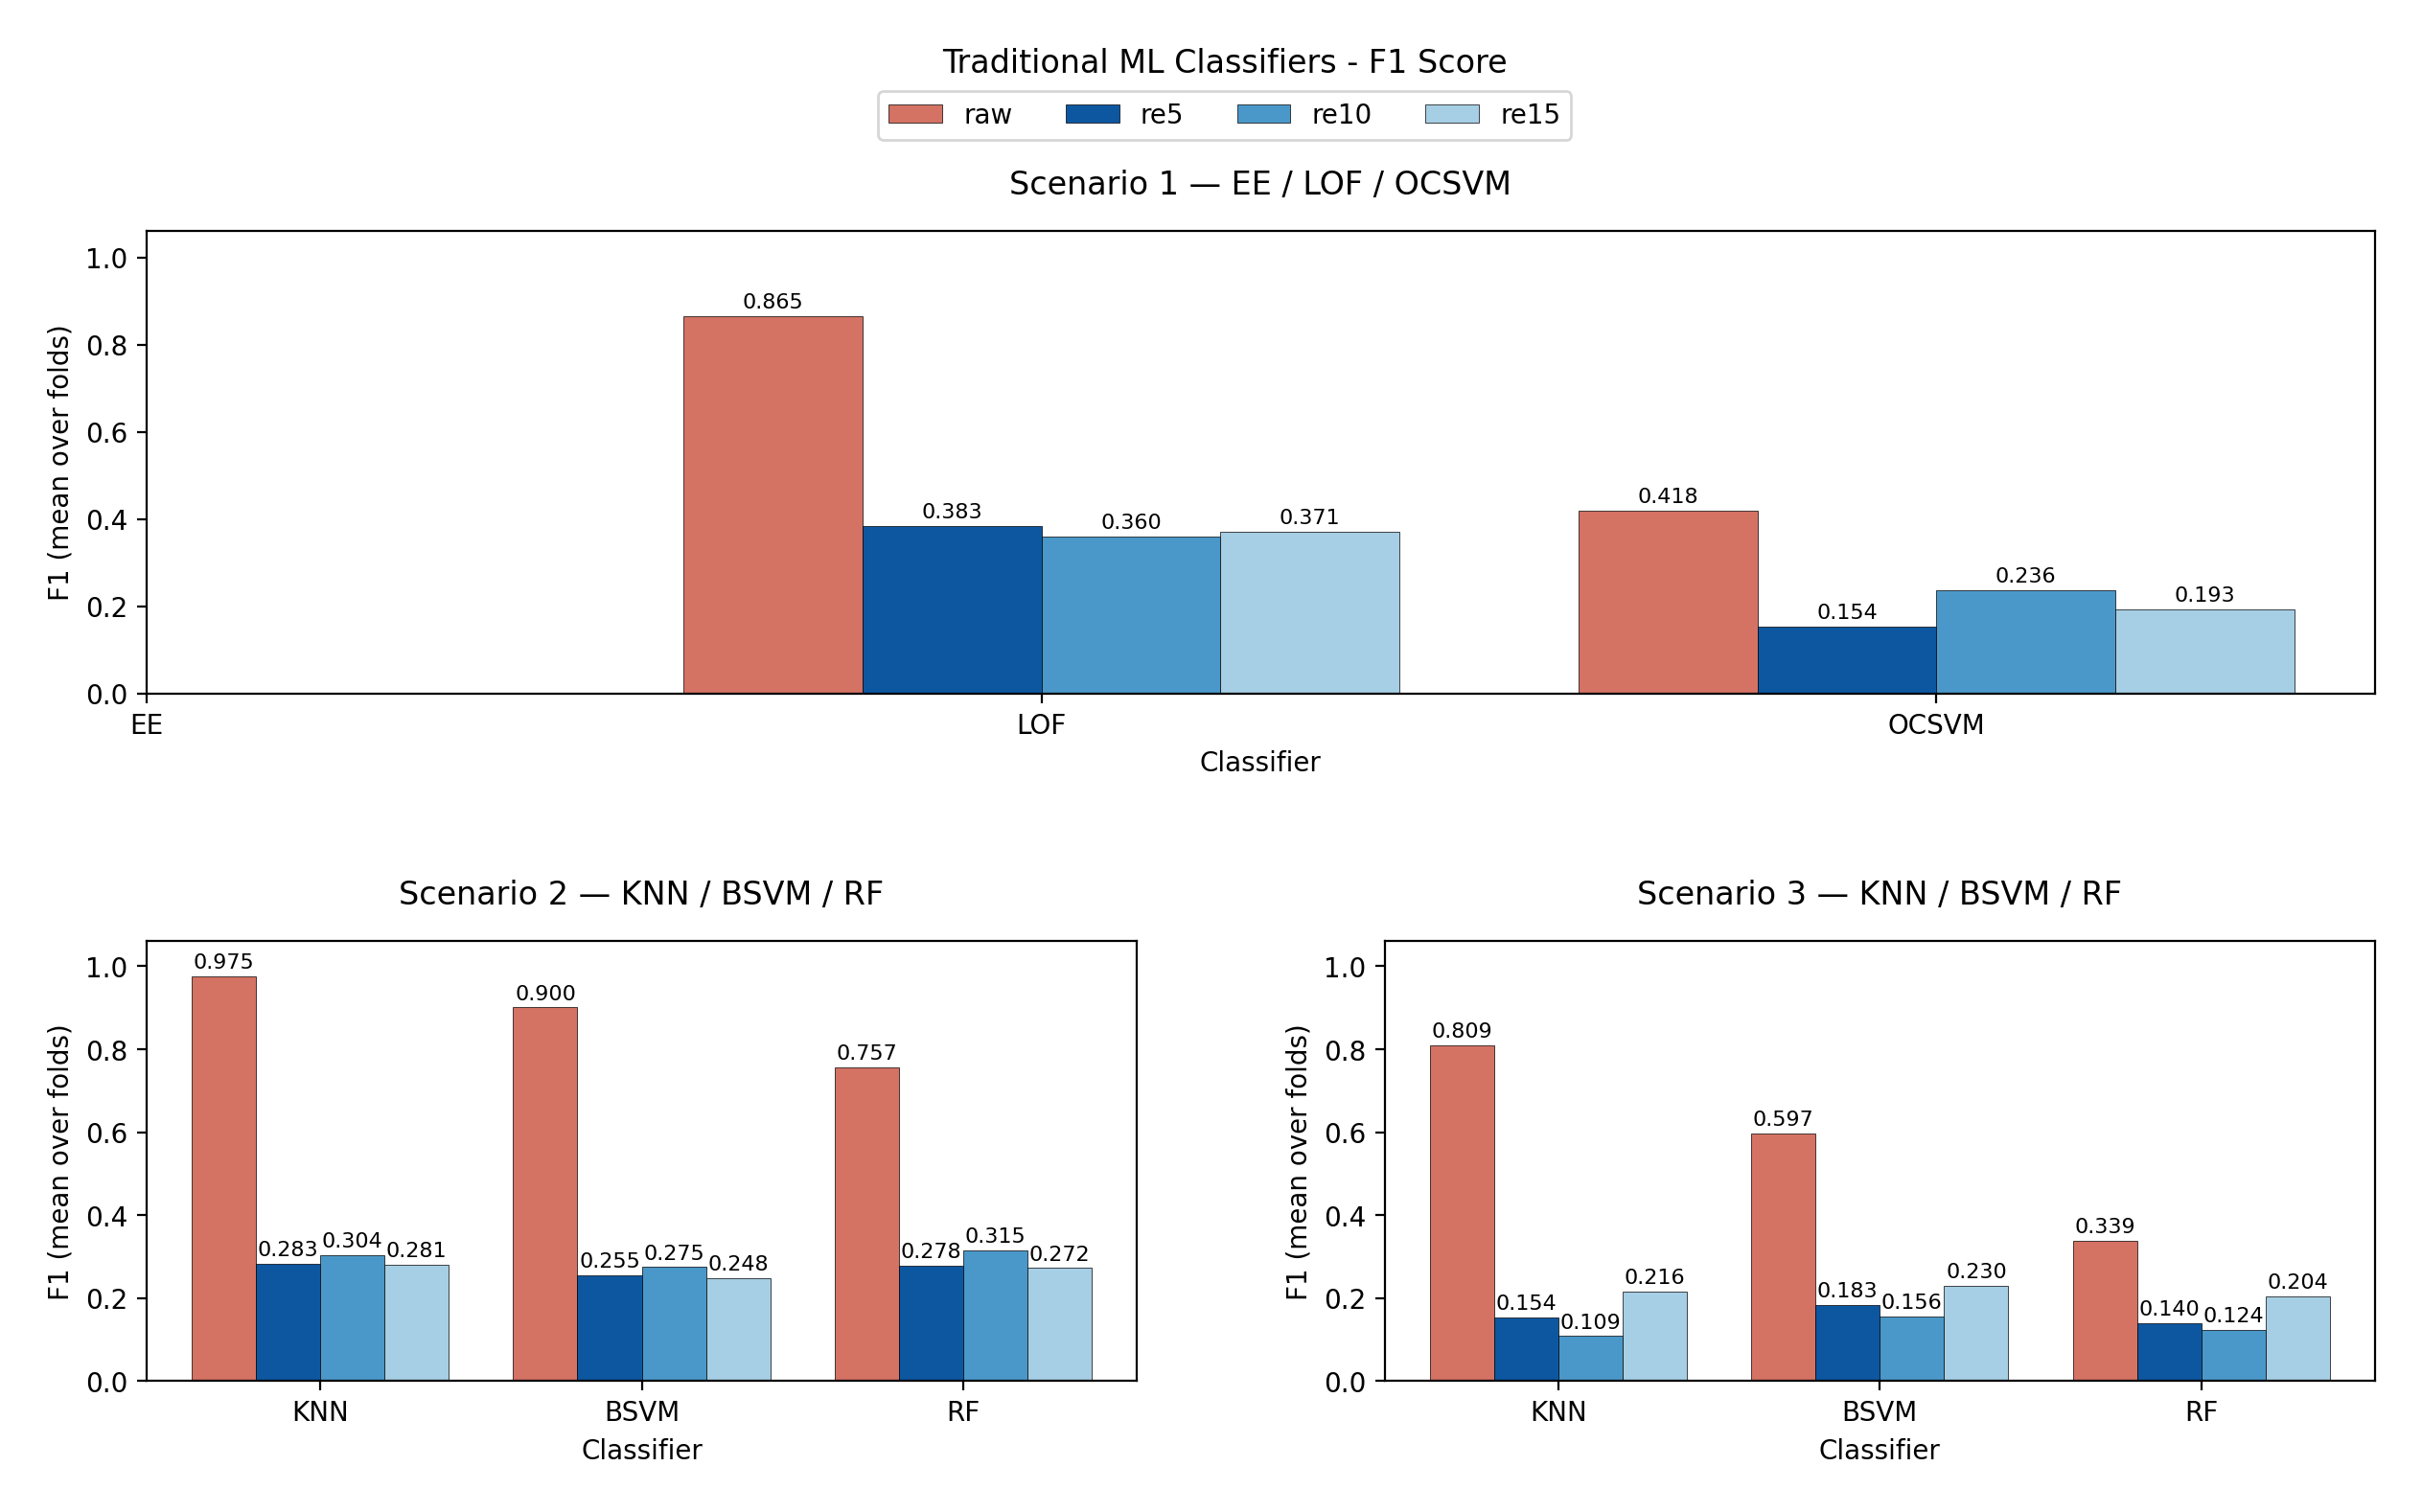
\includegraphics[width=\linewidth]{chapters/f1_custom_layout.png}
 \caption{Traditional ML Detection Methods F1-Score}
  \label{fig:tradML}
\end{figure}

figure \ref{fig:tradML} presents the mean F1-scores of the traditional machine learning
classifiers across the three evaluation scenarios. Scenario~1 evaluates
the one-class methods (Elliptic Envelope, \ac{LOF}, and One-Class \ac{SVM}),
whereas Scenarios~2 and~3 evaluate the supervised classifiers
(\ac{KNN}, Binary \ac{SVM}, and Random Forest). The different colors represent
the dataset representations (RAW, RE5, RE10, RE15).

For the RAW representation, \ac{LOF} achieves the strongest performance,
clearly outperforming Elliptic Envelope and One-Class \ac{SVM}.
In contrast, the latter two methods achieve only moderate performance.

When using the \ac{RE} representations, the performance
drops substantially for all one-class methods. In particular,
Elliptic Envelope fails to detect anomalies effectively, while
\ac{LOF} and One-Class \ac{SVM} achieve only low F1-scores. This indicates
that the reduced RE representations do not provide sufficient
discriminative information for one-class modeling.

In Scenario~2, all supervised classifiers achieve high F1-scores
when operating on the RAW representation. \ac{KNN} performs best,
followed closely by Binary \ac{SVM} and Random Forest.

However, when switching to \ac{RE}-based representations, performance
decreases significantly across all classifiers. Although minor
variations exist between RE5, RE10, and RE15, the results remain
consistently below the RAW baseline. This suggests that the full
packet structure contains important discriminative features that
are partially lost in the \ac{RE} representations.

Scenario~3 introduces previously unseen attack types during testing.
For the RAW representation, all supervised classifiers exhibit
a noticeable drop in performance compared to Scenario~2,
with \ac{KNN} remaining the strongest model.

Using the \ac{RE} representations further degrades performance.
In this setting, several classifiers approach near-random
behavior.


\subsection{Ensemble Classifier Results}

\begin{figure}[!htbp]
	\centering
	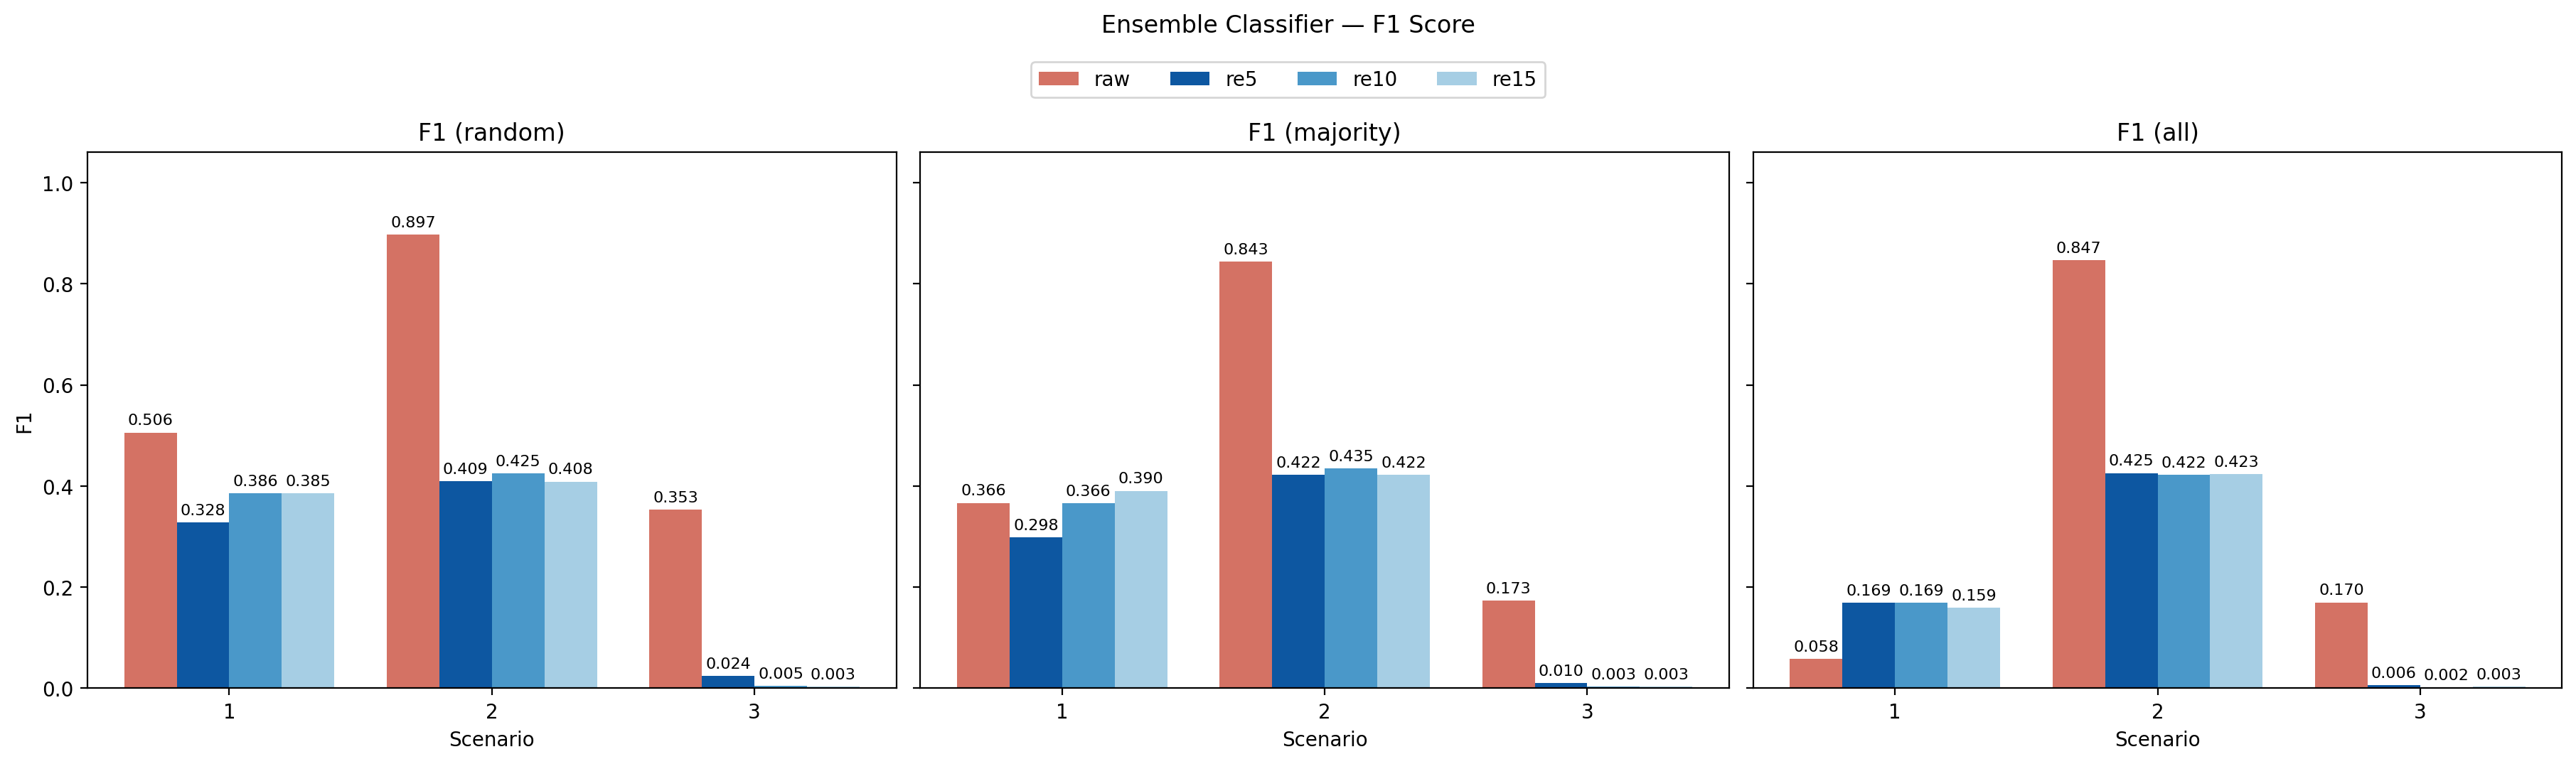
\includegraphics[width=\linewidth]{chapters/ec_all_representations_f1.png}
	\caption{Ensemble Classifier F1-Score}
 \label{fig:ec}
\end{figure}

figure \ref{fig:ec} shows the mean F1-scores of the ensemble classifier under
the three aggregation modes (random, majority, all) across all
dataset representations and evaluation scenarios.

Across all representations and aggregation modes, a consistent
difficulty ordering can be observed: Scenario~2 achieves the best
performance, Scenario~1 yields intermediate results, and Scenario~3
consistently performs worst. This pattern is stable across RAW and
all reverse-engineered representations, indicating that the scenario
characteristics have a stronger impact on performance than the
chosen ensemble strategy.

In particular, Scenario~3 leads to a substantial drop in F1-score
for all dataset types, reflecting the difficulty of generalizing
to highly constrained or unseen attack configurations.

For the RAW representation, the random and majority strategies
perform similarly and achieve strong results in Scenario~2.
In contrast, the \emph{all} strategy often leads to a noticeable
performance decrease, especially in Scenario~1. This behavior
suggests that at least one weak base classifier negatively
influences the ensemble when unanimity is required.

Overall, majority voting provides the most stable behavior
across scenarios, while the \emph{all} strategy appears overly
restrictive.

A clear performance gap is visible between RAW and all
reverse-engineered representations. The RAW dataset consistently
achieves substantially higher F1-scores across all scenarios and
ensemble modes.

The reverse-engineered representations (RE5, RE10, RE15) show
comparable behavior among each other, with RE15 generally yielding
the strongest results within this group. Nevertheless, their
performance remains significantly below that of the RAW data.


\clearpage
\subsection{Feature Importance}
To better understand which components of the 32-dimensional latent
feature vector drive the classification decisions, we analyze feature
importance for each traditional ML model. Each panel in the following
figures corresponds to one classifier and displays the importance
scores for all 32 features ($f_0$–$f_{31}$).

Since importance definitions differ between models and
are normalized independently (see \ref{subsubsec:feature_importance}), values should primarily be interpreted
within each classifier rather than compared directly across models.

Positive importance values indicate that a feature contributes
positively to correct classification performance, whereas negative
values indicate that permuting the feature improves performance,
suggesting that the feature may introduce noise or misleading signals.

\begin{figure}[!htbp]
	\centering
	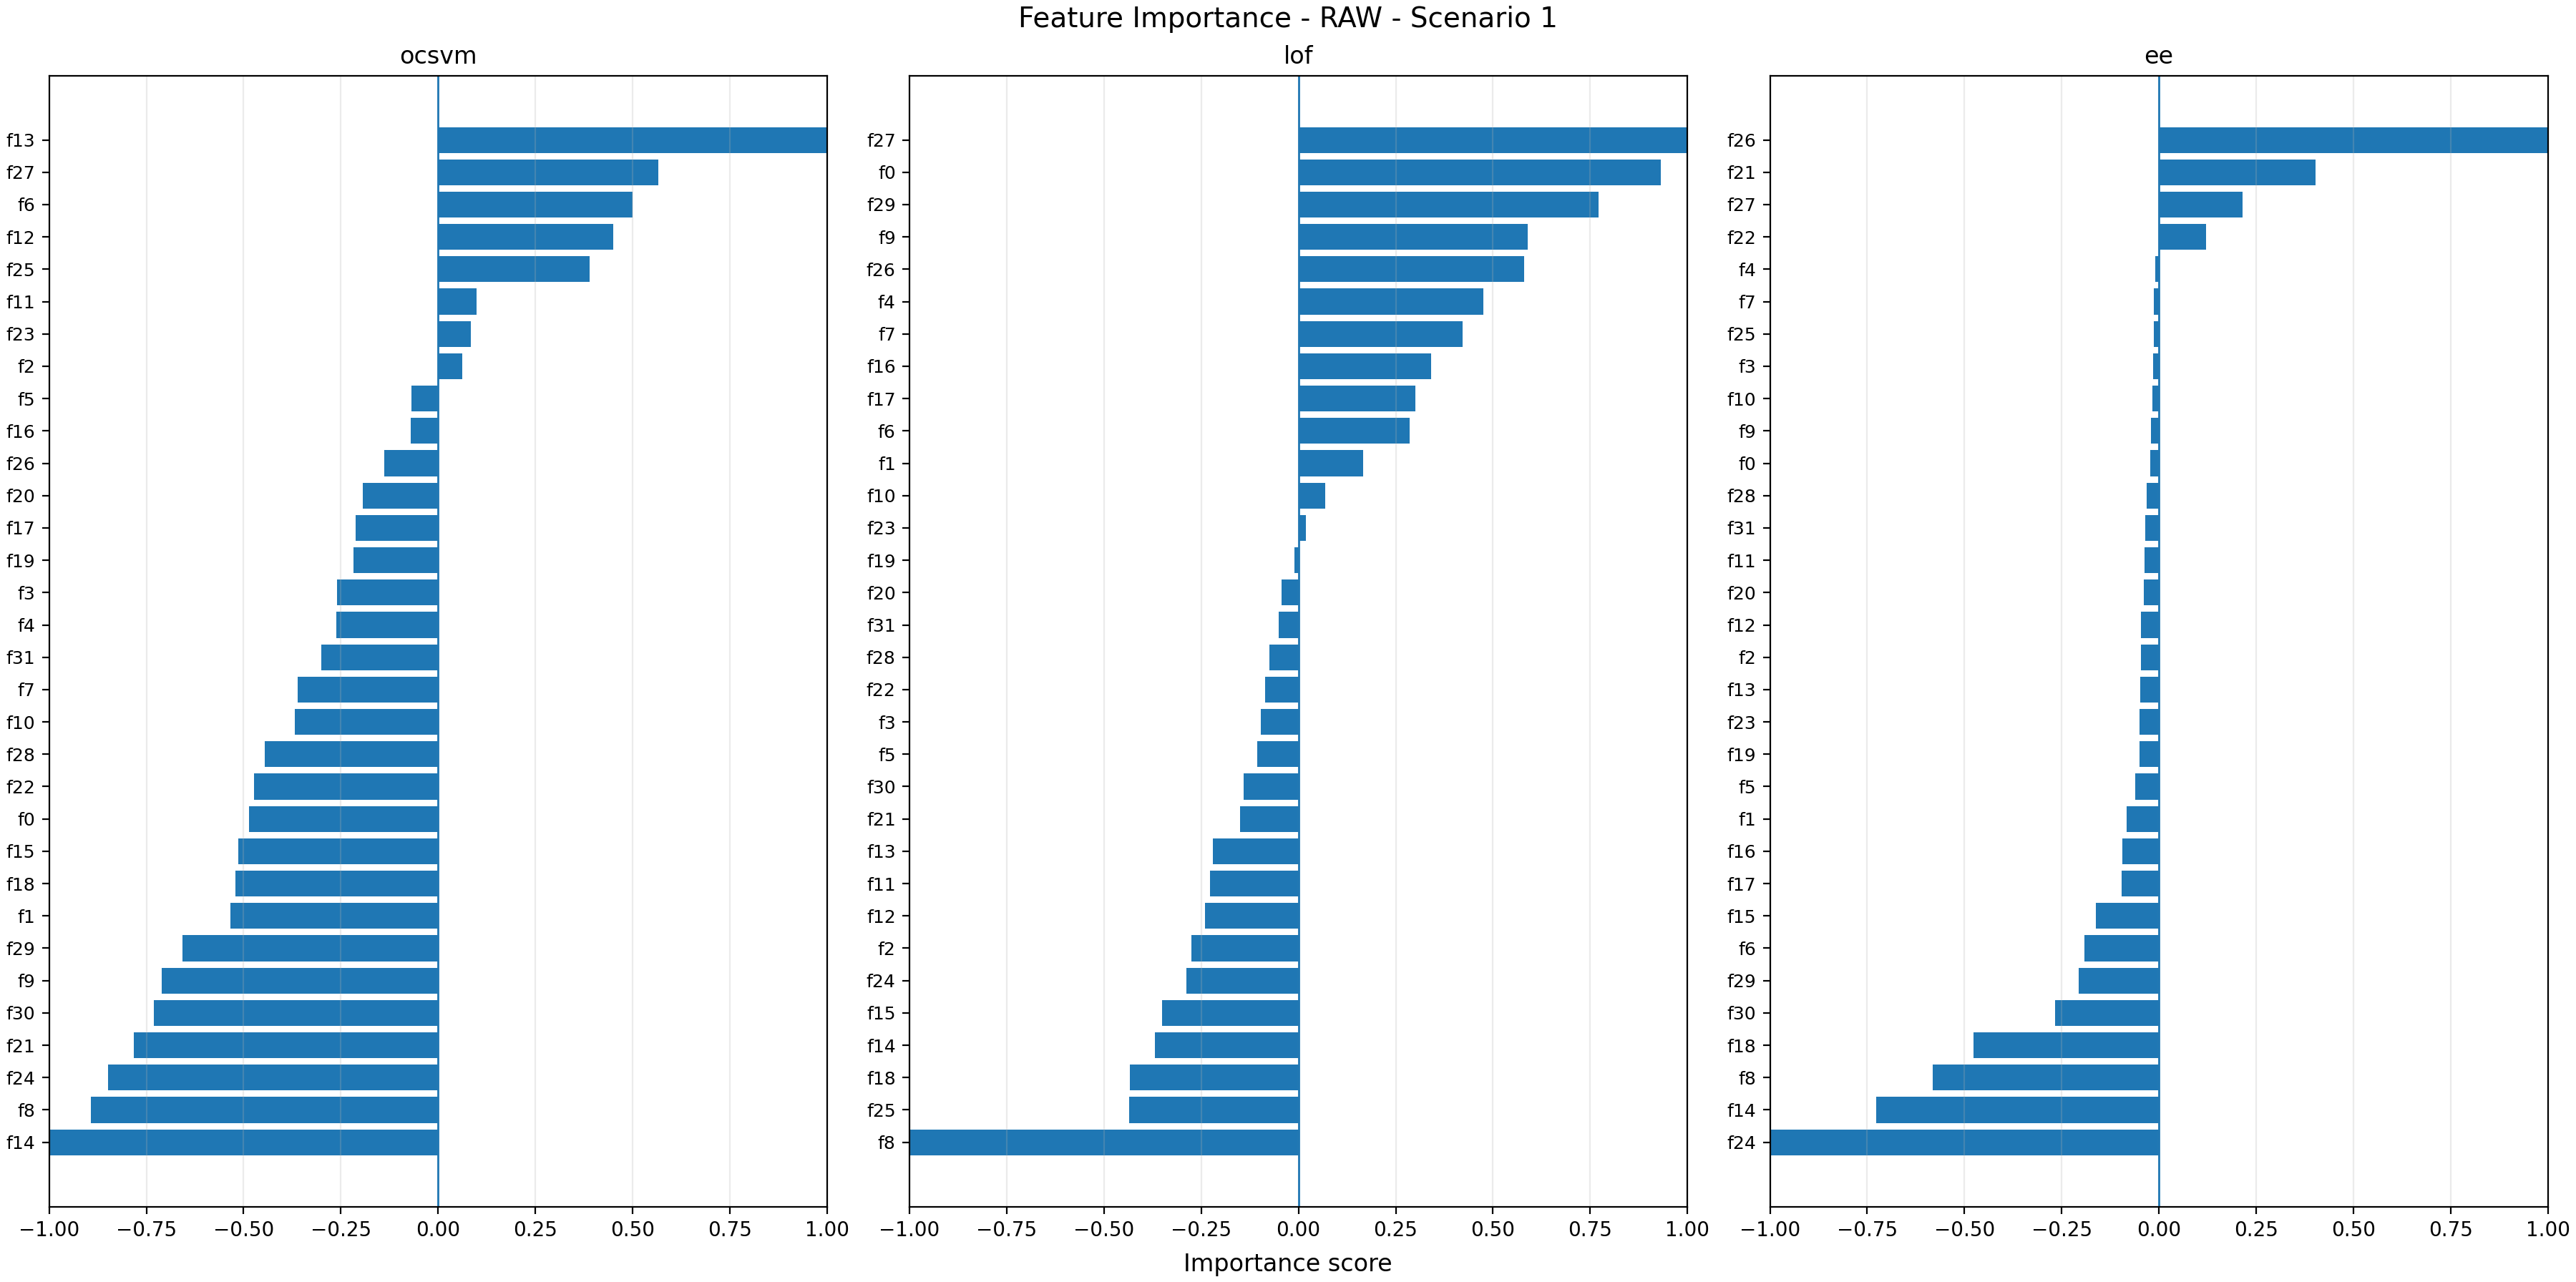
\includegraphics[width=\linewidth]{chapters/fi_helpful_panels_raw_s1.png}
	\caption{Feature Importance — RAW, Scenario 1}
	\label{fig:fi-raw-s1}
\end{figure}

For the RAW representation in Scenario~1 (see \cref{fig:fi-raw-s1}),
several consistent patterns emerge across the one-class models.
In particular, $f_{27}$ appears among the most helpful features
for all classifiers, whereas $f_{14}$ and $f_{8}$ are consistently
ranked among the most harmful.

\ac{OCSVM} and \ac{EE} rely strongly on a small number of dominant features
(\ac{OCSVM}: $f_{13}$; \ac{EE}: $f_{26}$), while \ac{LOF} distributes importance
more broadly across multiple components of the latent vector.
Furthermore, clear sign disagreements occur between classifiers,
indicating that the one-class methods extract different structural
aspects from the same feature space.

\begin{figure}[!htbp]
	\centering
	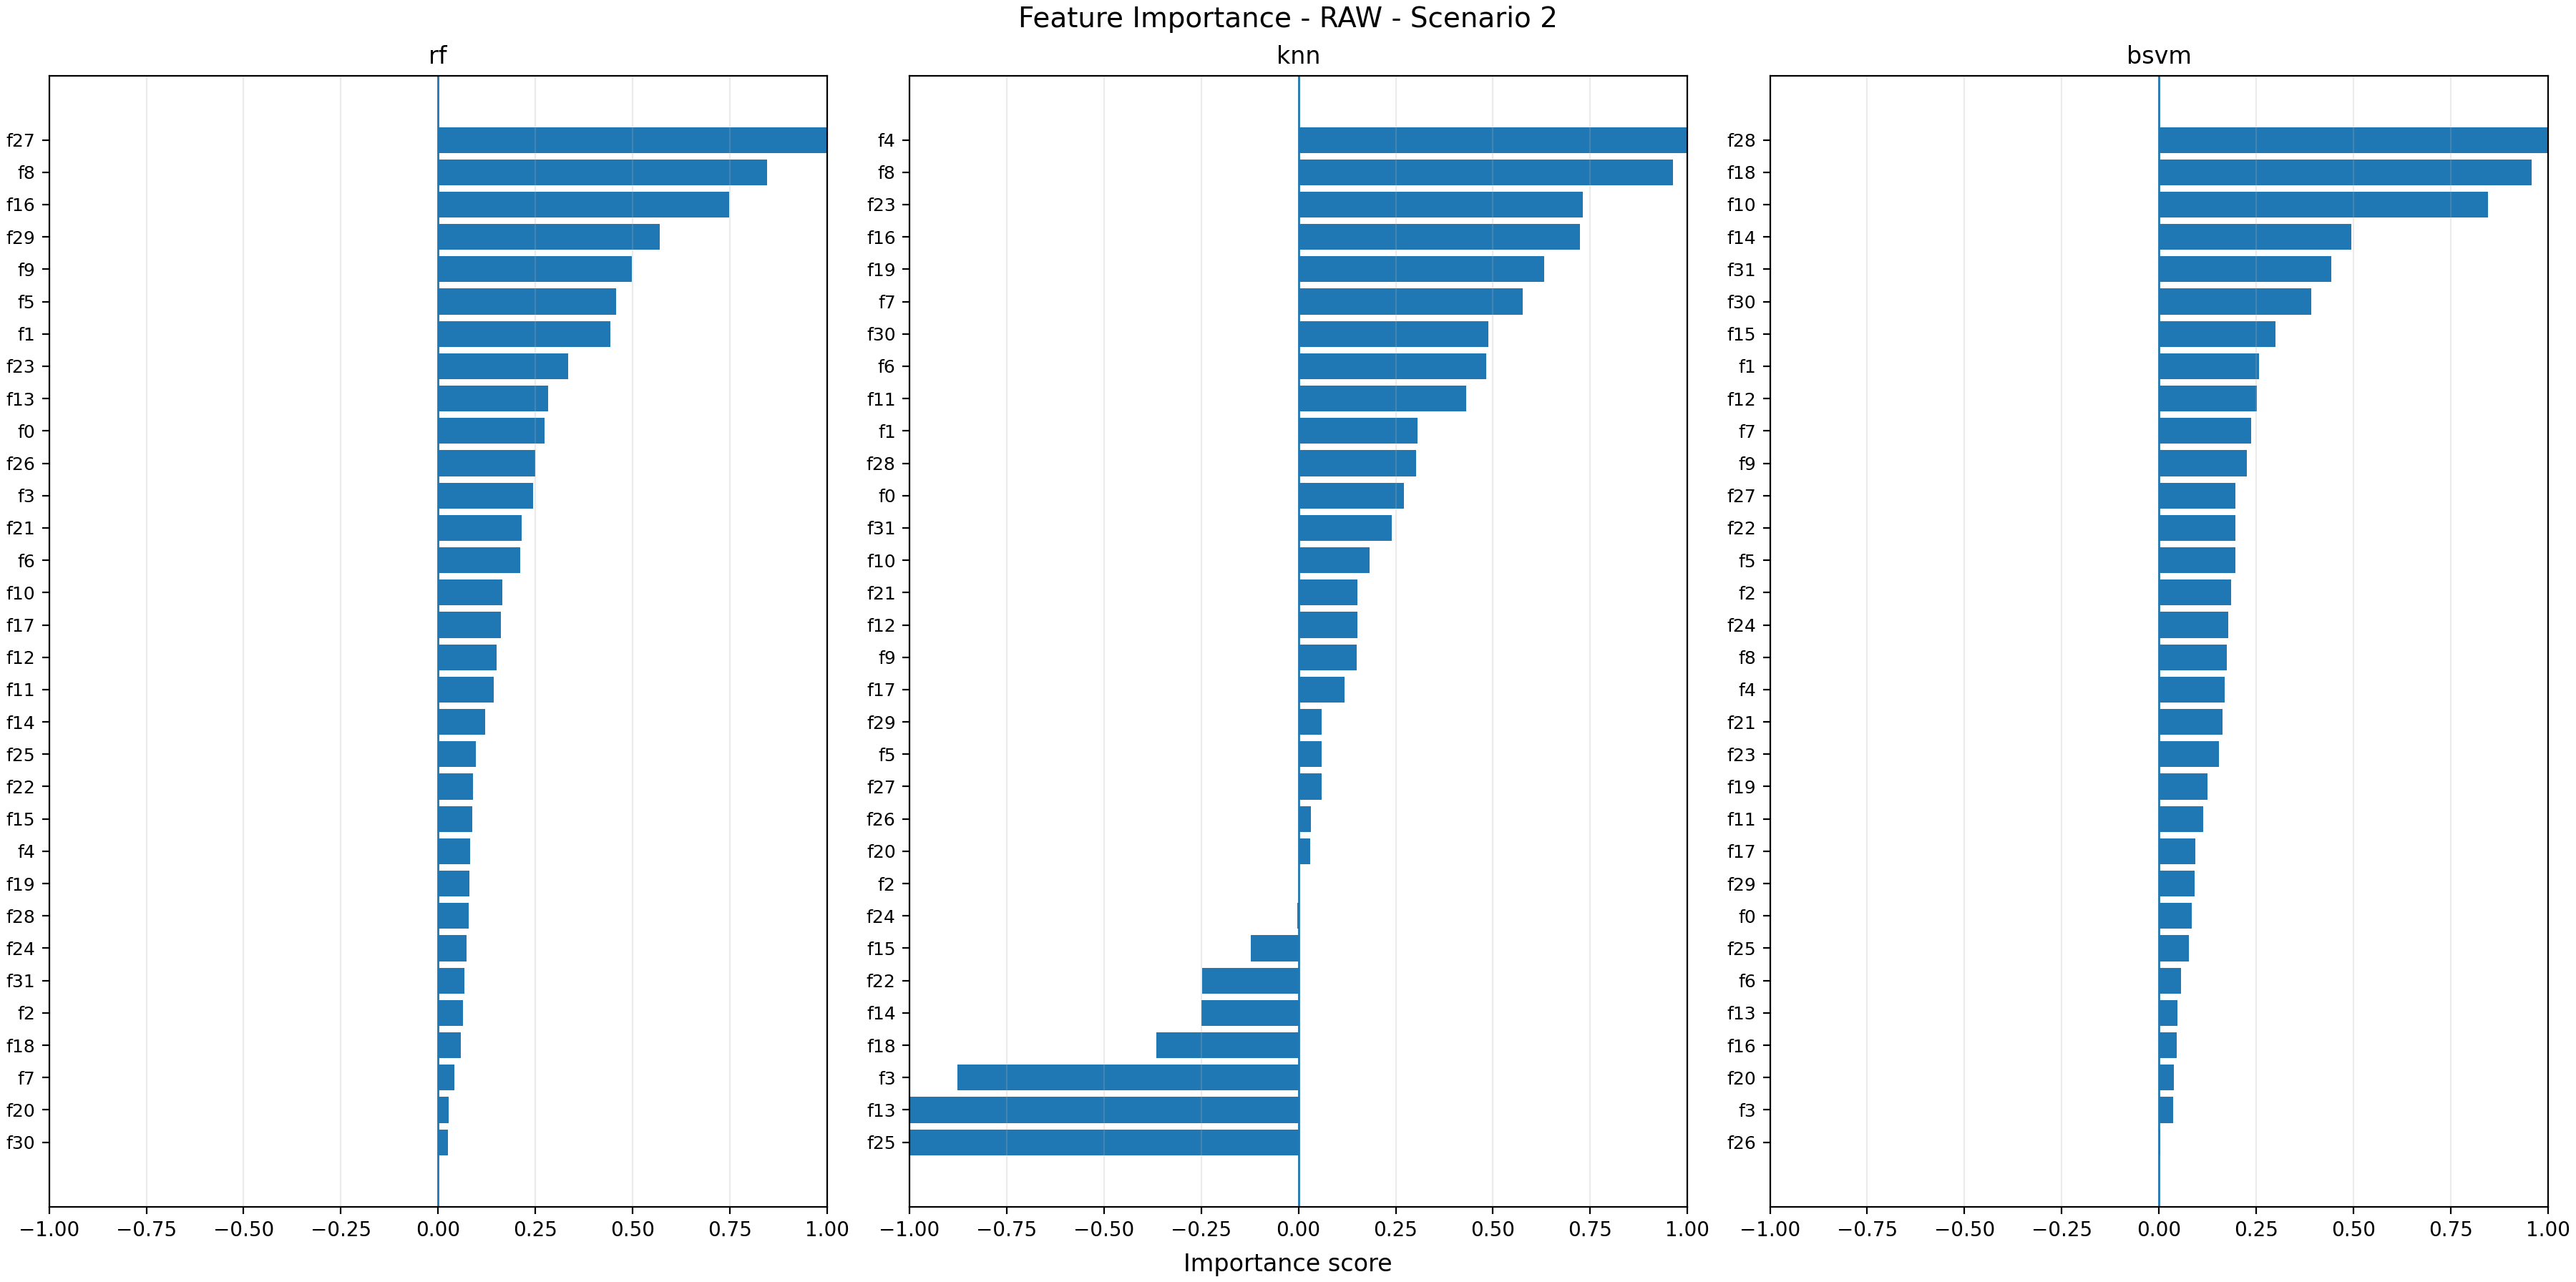
\includegraphics[width=\linewidth]{chapters/fi_helpful_panels_raw_s2.png}
	\caption{Feature Importance — RAW, Scenario 2}
	\label{fig:fi-raw-s2}
\end{figure}

In the supervised setting of Scenario~2 (\cref{fig:fi-raw-s2}),
Random Forest is dominated by a relatively small subset of features,
most prominently $f_{27}$, followed by $f_{8}$ and $f_{16}$.
\ac{KNN} exhibits a more polarized structure with both strongly positive
and strongly negative contributions, reflecting a selective reliance
on specific latent dimensions.

Binary \ac{SVM} emphasizes a partially different subset of features,
suggesting that the linear decision boundary captures directions
in the latent space that differ from those exploited by tree-based
or neighbor-based models.

\begin{figure}[!htbp]
	\centering
	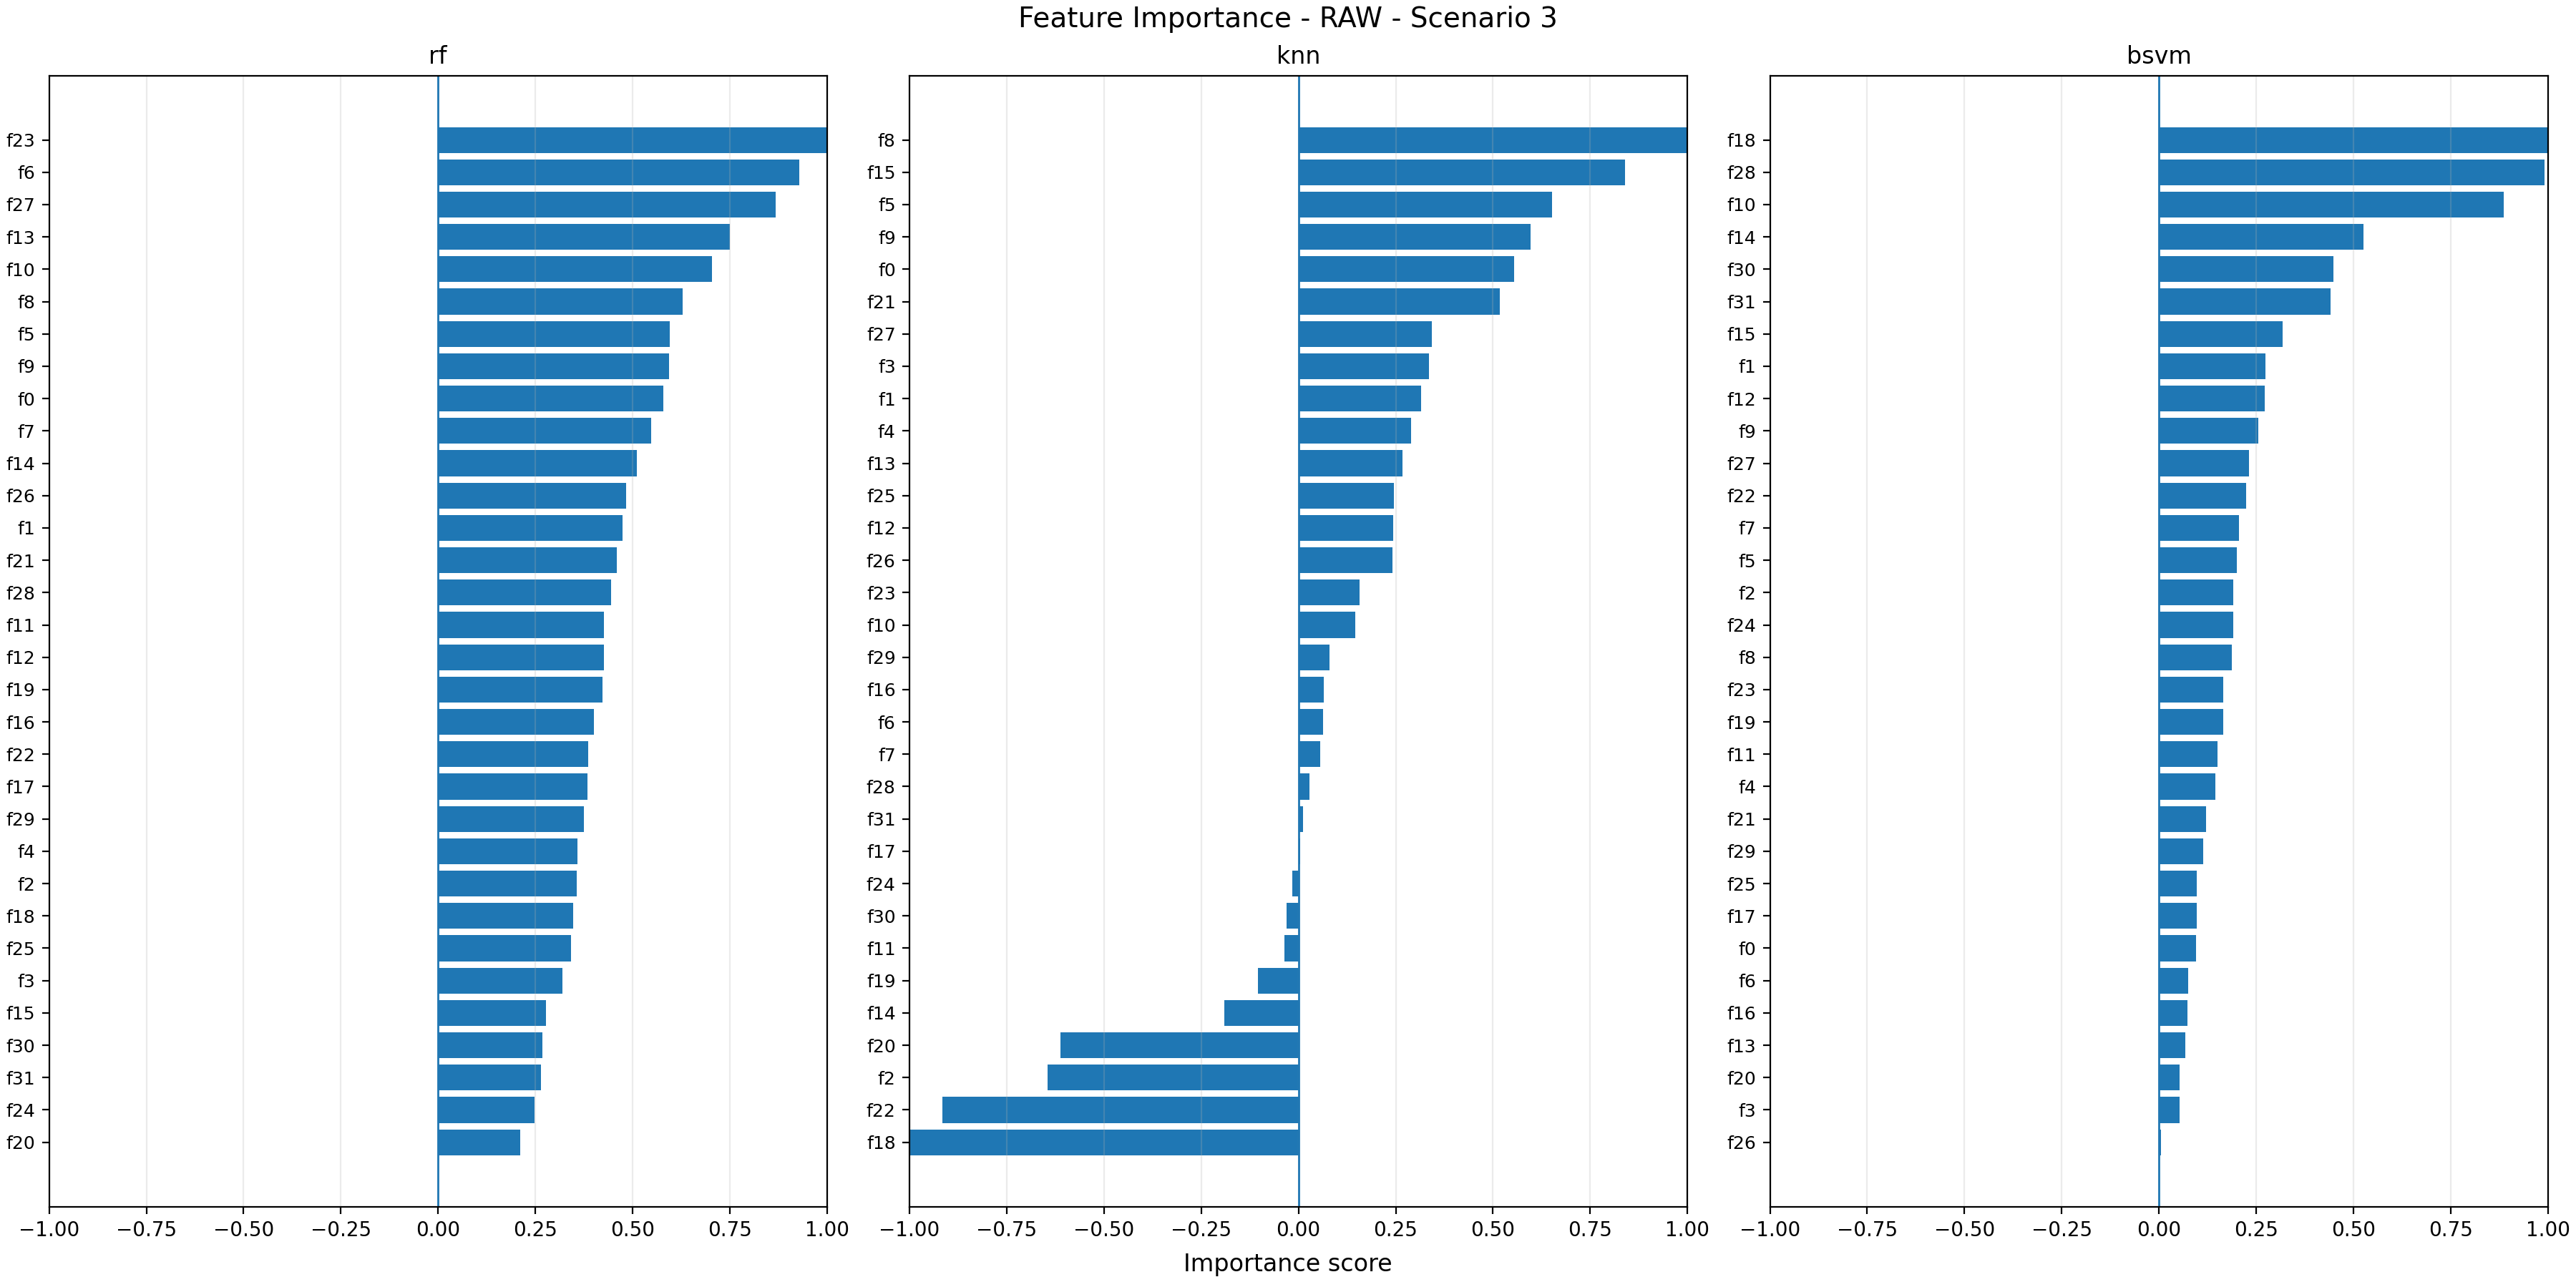
\includegraphics[width=\linewidth]{chapters/fi_helpful_panels_raw_s3.png}
	\caption{Feature Importance — RAW, Scenario 3}
	\label{fig:fi-raw-s3}
\end{figure}
\clearpage

Under the more challenging generalization setting of Scenario~3
(\cref{fig:fi-raw-s3}), importance patterns become more concentrated.
Random Forest highlights a compact group of dominant features,
while \ac{KNN} again shows strong positive and negative contributions.
Binary \ac{SVM} focuses on a limited subset of high-weight components.

Notably, certain features such as $f_{27}$ and $f_{8}$ remain
consistently relevant across classifiers, indicating that specific
latent dimensions retain discriminative power even when attack
types differ between training and testing.

\begin{figure}[!htbp]
	\centering
	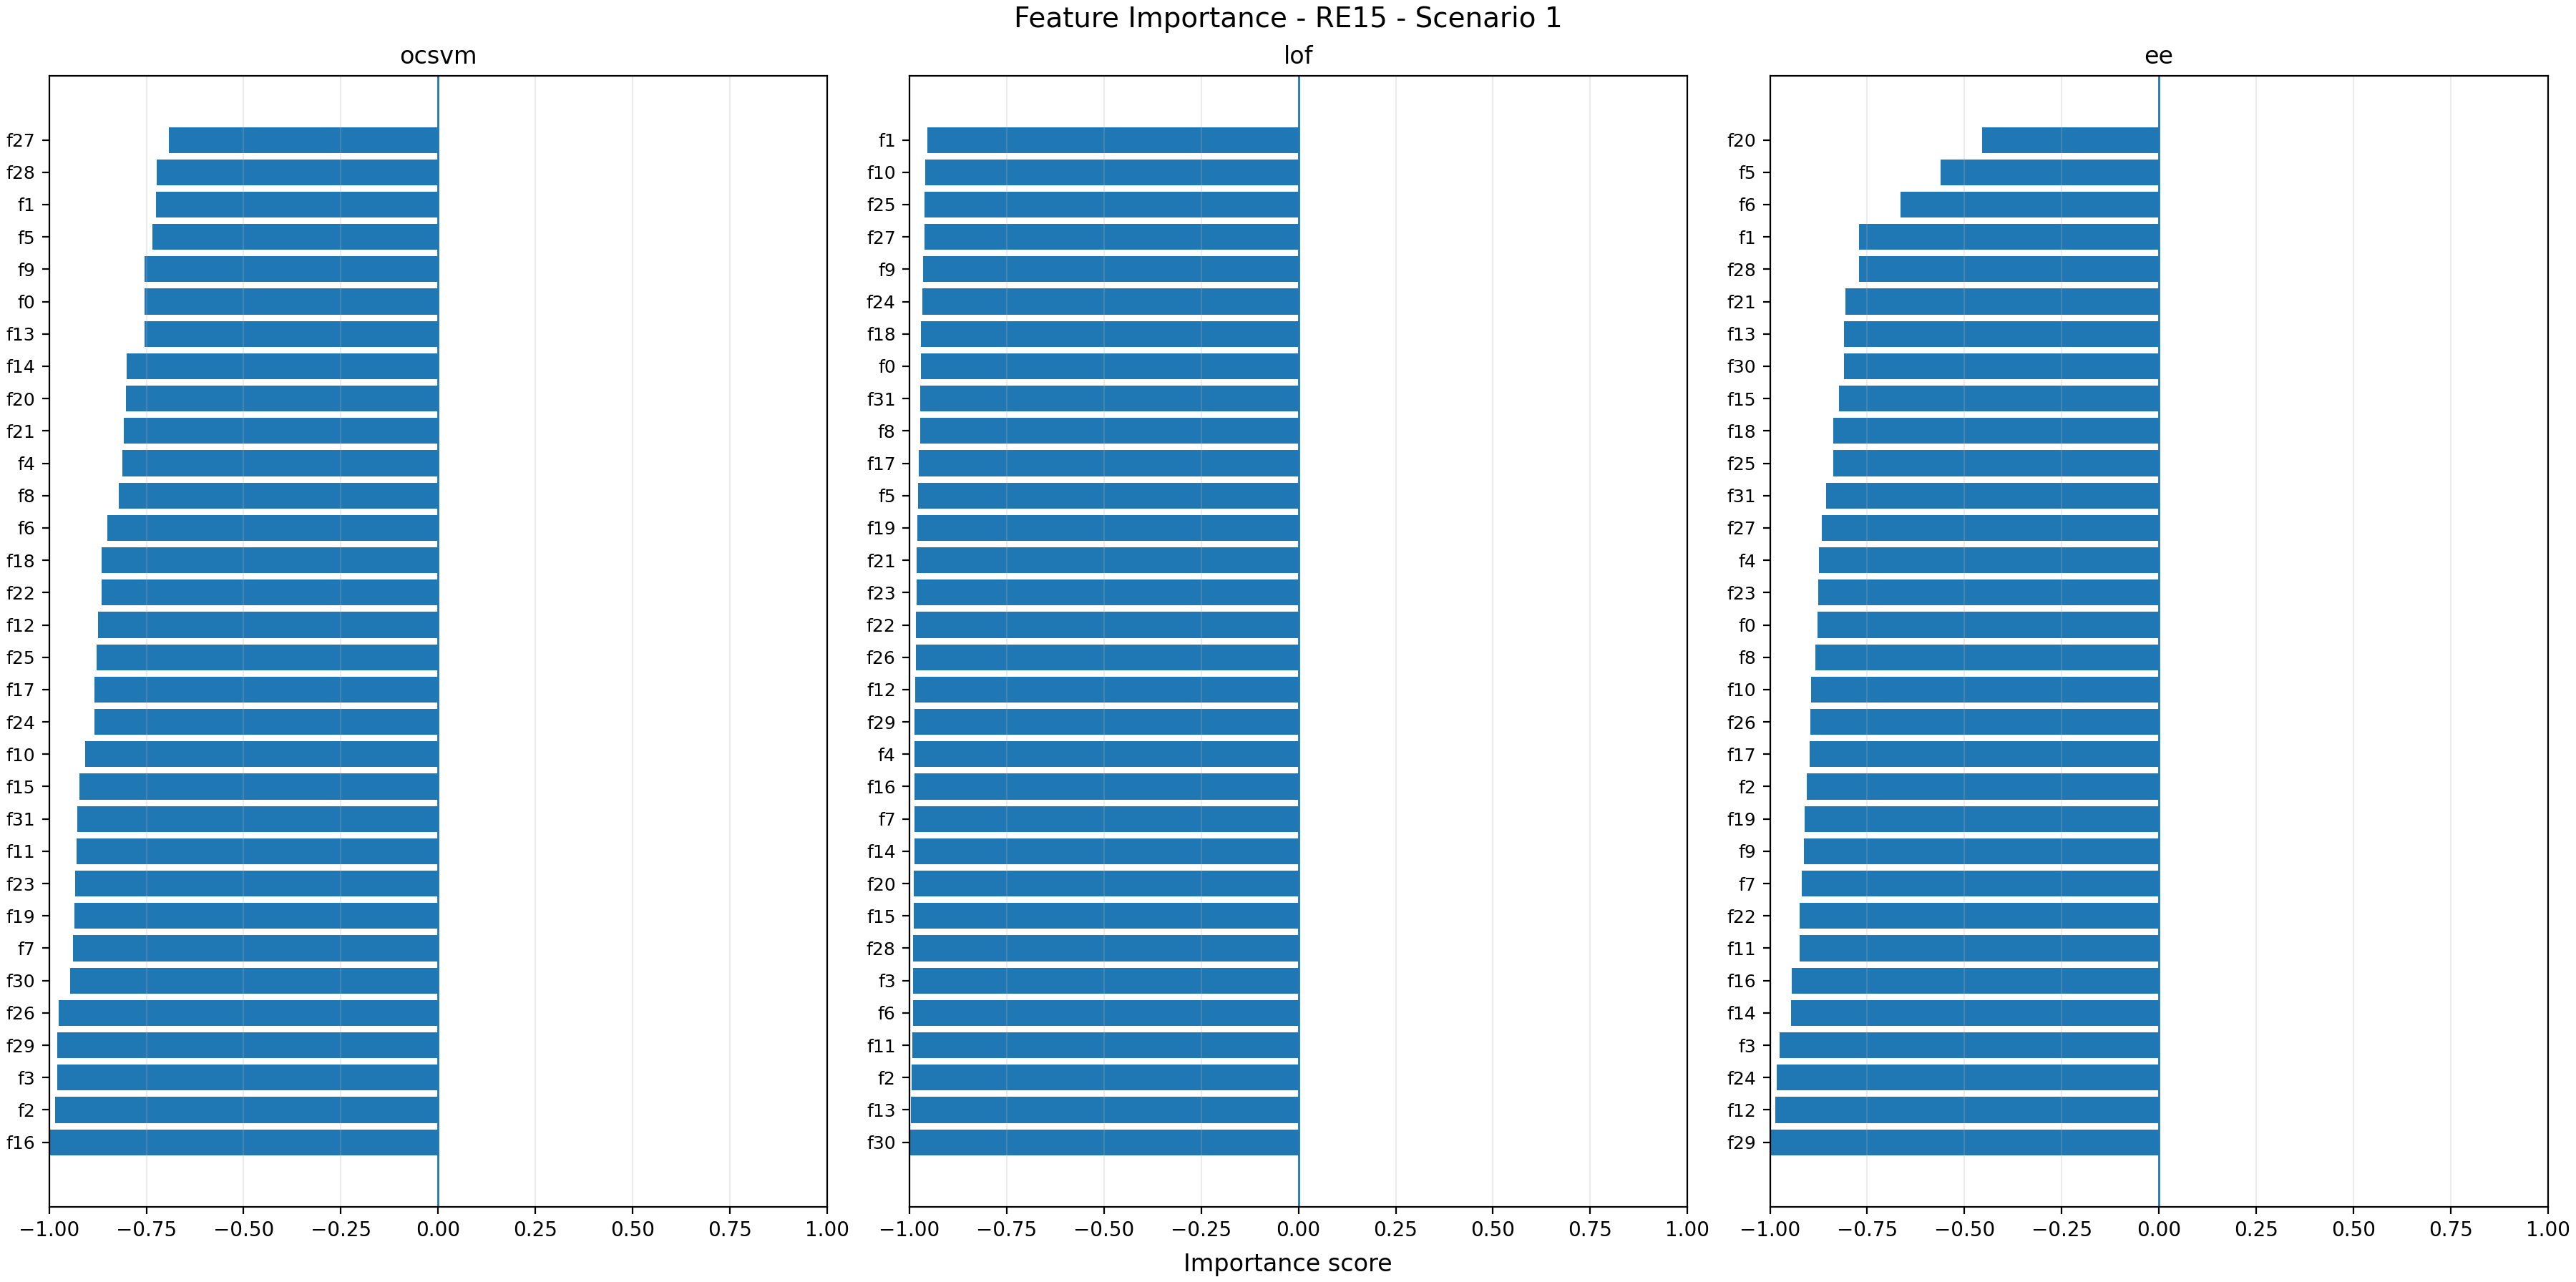
\includegraphics[width=\linewidth]{chapters/fi_helpful_panels_re15_s1.png}
	\caption{Feature Importance — RE15, Scenario 1}
	\label{fig:fi-re15-s1}
\end{figure}

For the RE15 representation in Scenario~1
(\cref{fig:fi-re15-s1}), the pattern differs markedly from RAW.
Nearly all features receive negative importance values across
classifiers, and no clearly beneficial subset emerges.
This indicates that the reverse-engineered representation does not
provide strong discriminative structure for one-class detection
in this configuration.

\begin{figure}[!htbp]
	\centering
	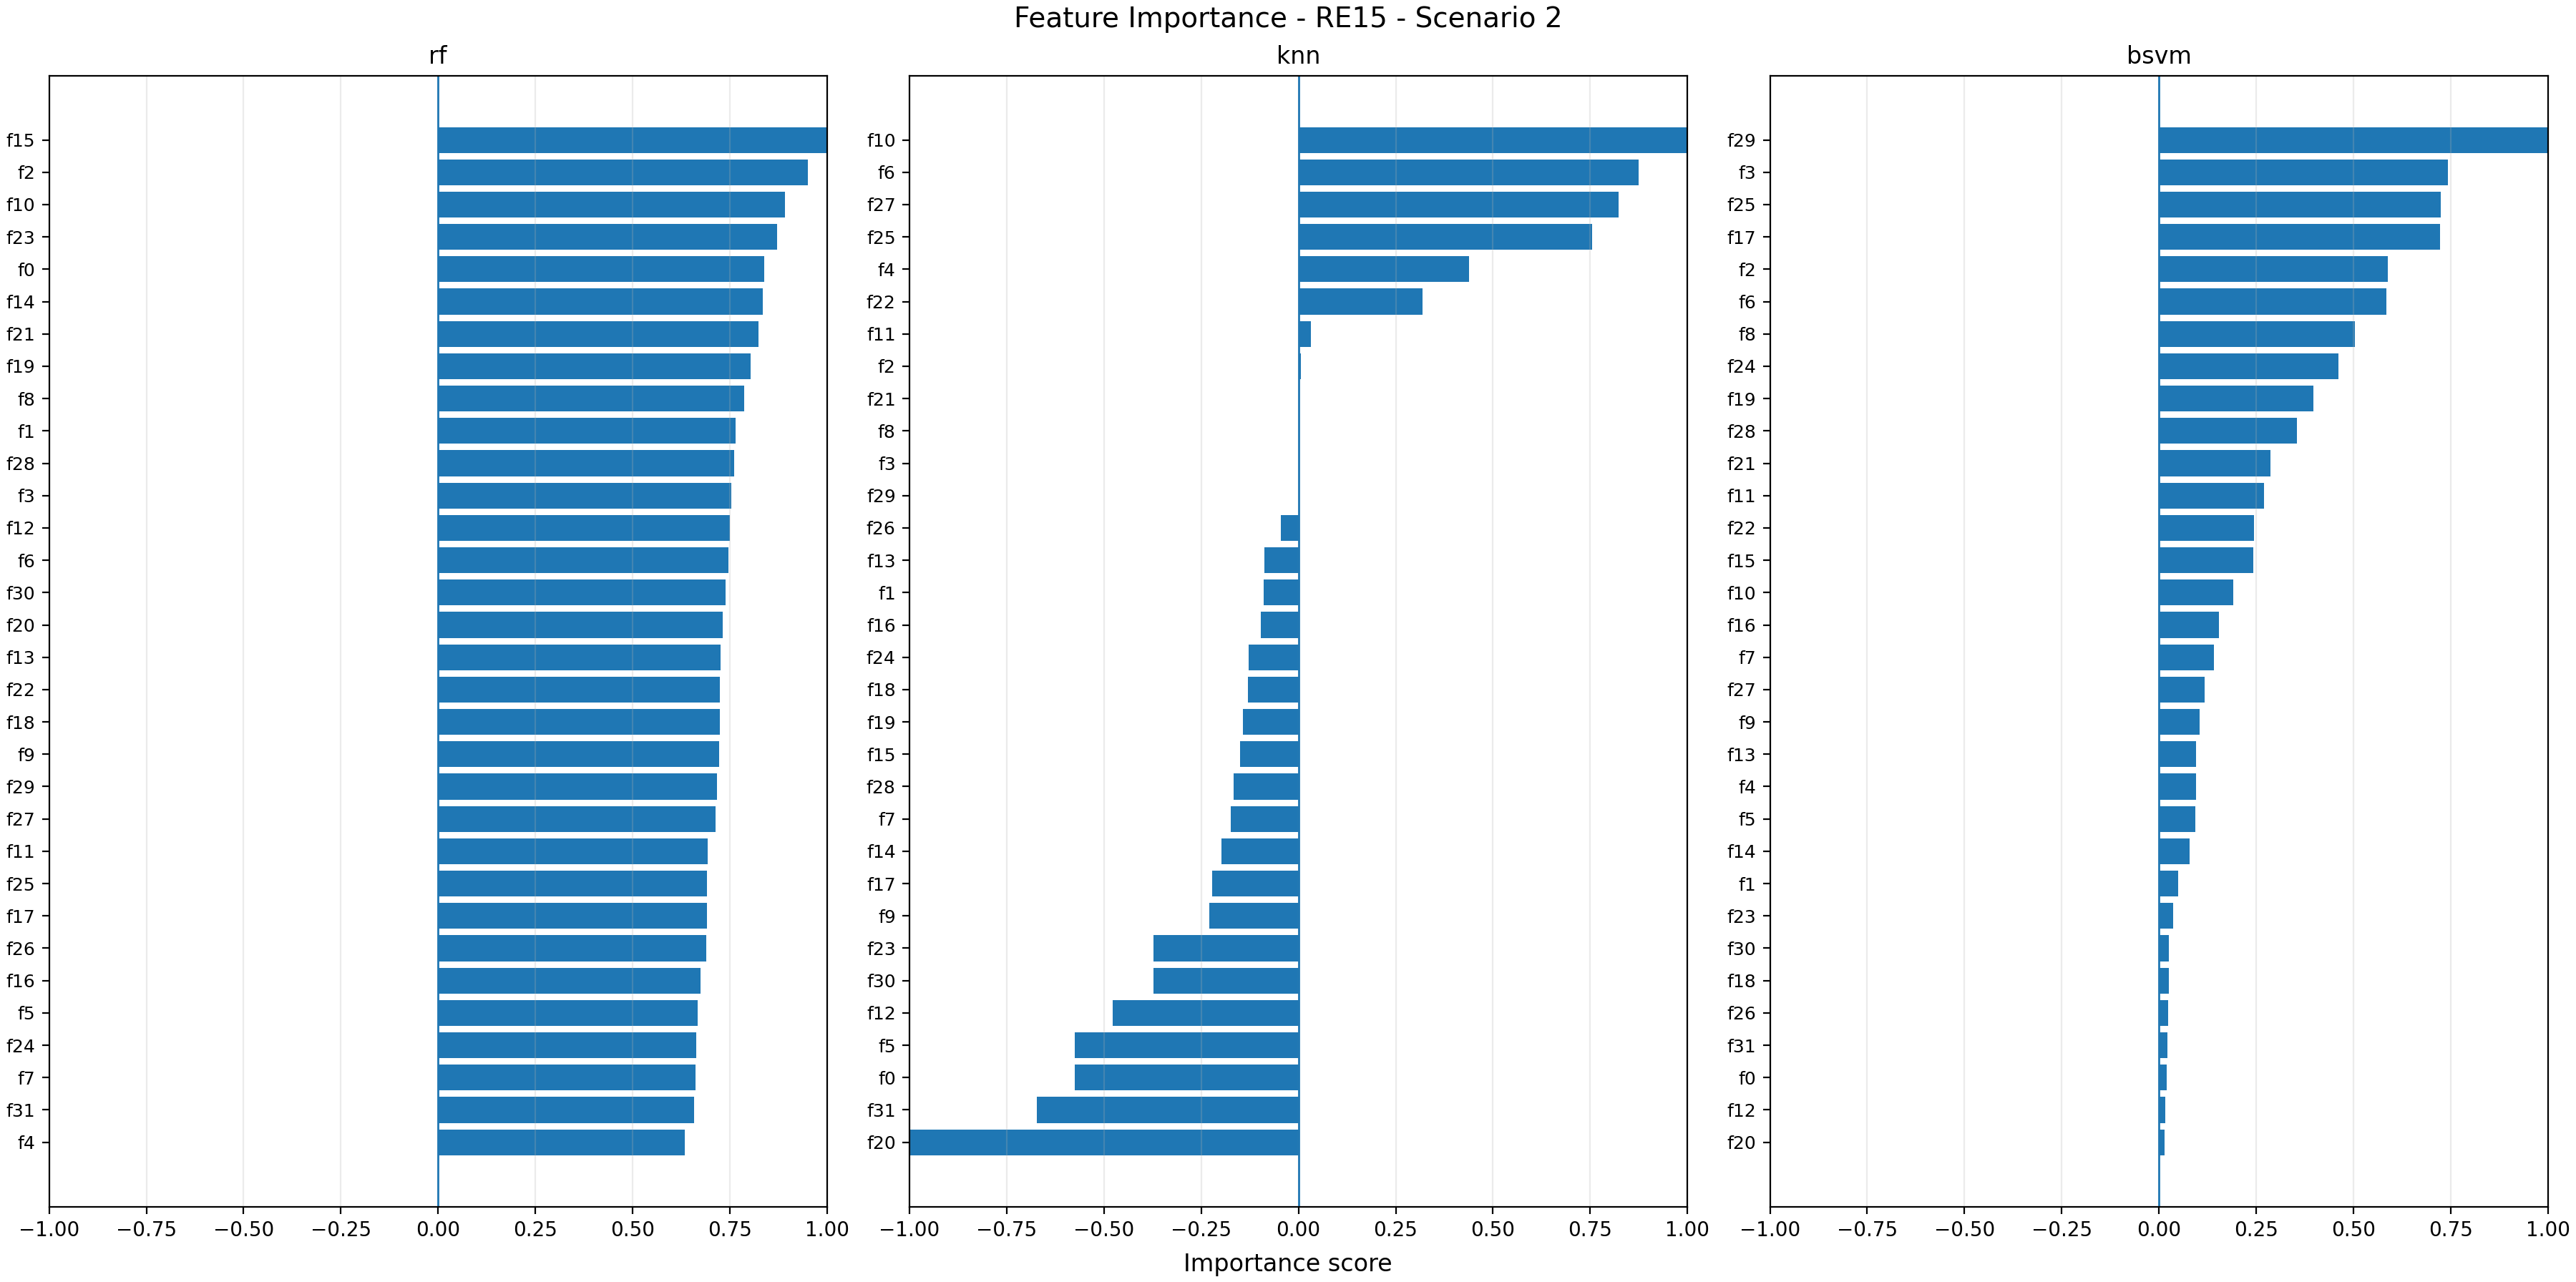
\includegraphics[width=\linewidth]{chapters/fi_helpful_panels_re15_s2.png}
	\caption{Feature Importance — RE15, Scenario 2}
	\label{fig:fi-re15-s2}
\end{figure}

In Scenario~2 with RE15 (\cref{fig:fi-re15-s2}), the classifiers
exhibit more differentiated behavior.
Random Forest distributes importance relatively broadly,
\ac{KNN} again separates helpful from harmful features,
and Binary \ac{SVM} concentrates on a smaller subset of dominant weights.

Although limited cross-model overlap exists (e.g., $f_{10}$ appears
relevant for multiple classifiers), overall agreement between models
is weaker than observed for the RAW representation.

\begin{figure}[!htbp]
	\centering
	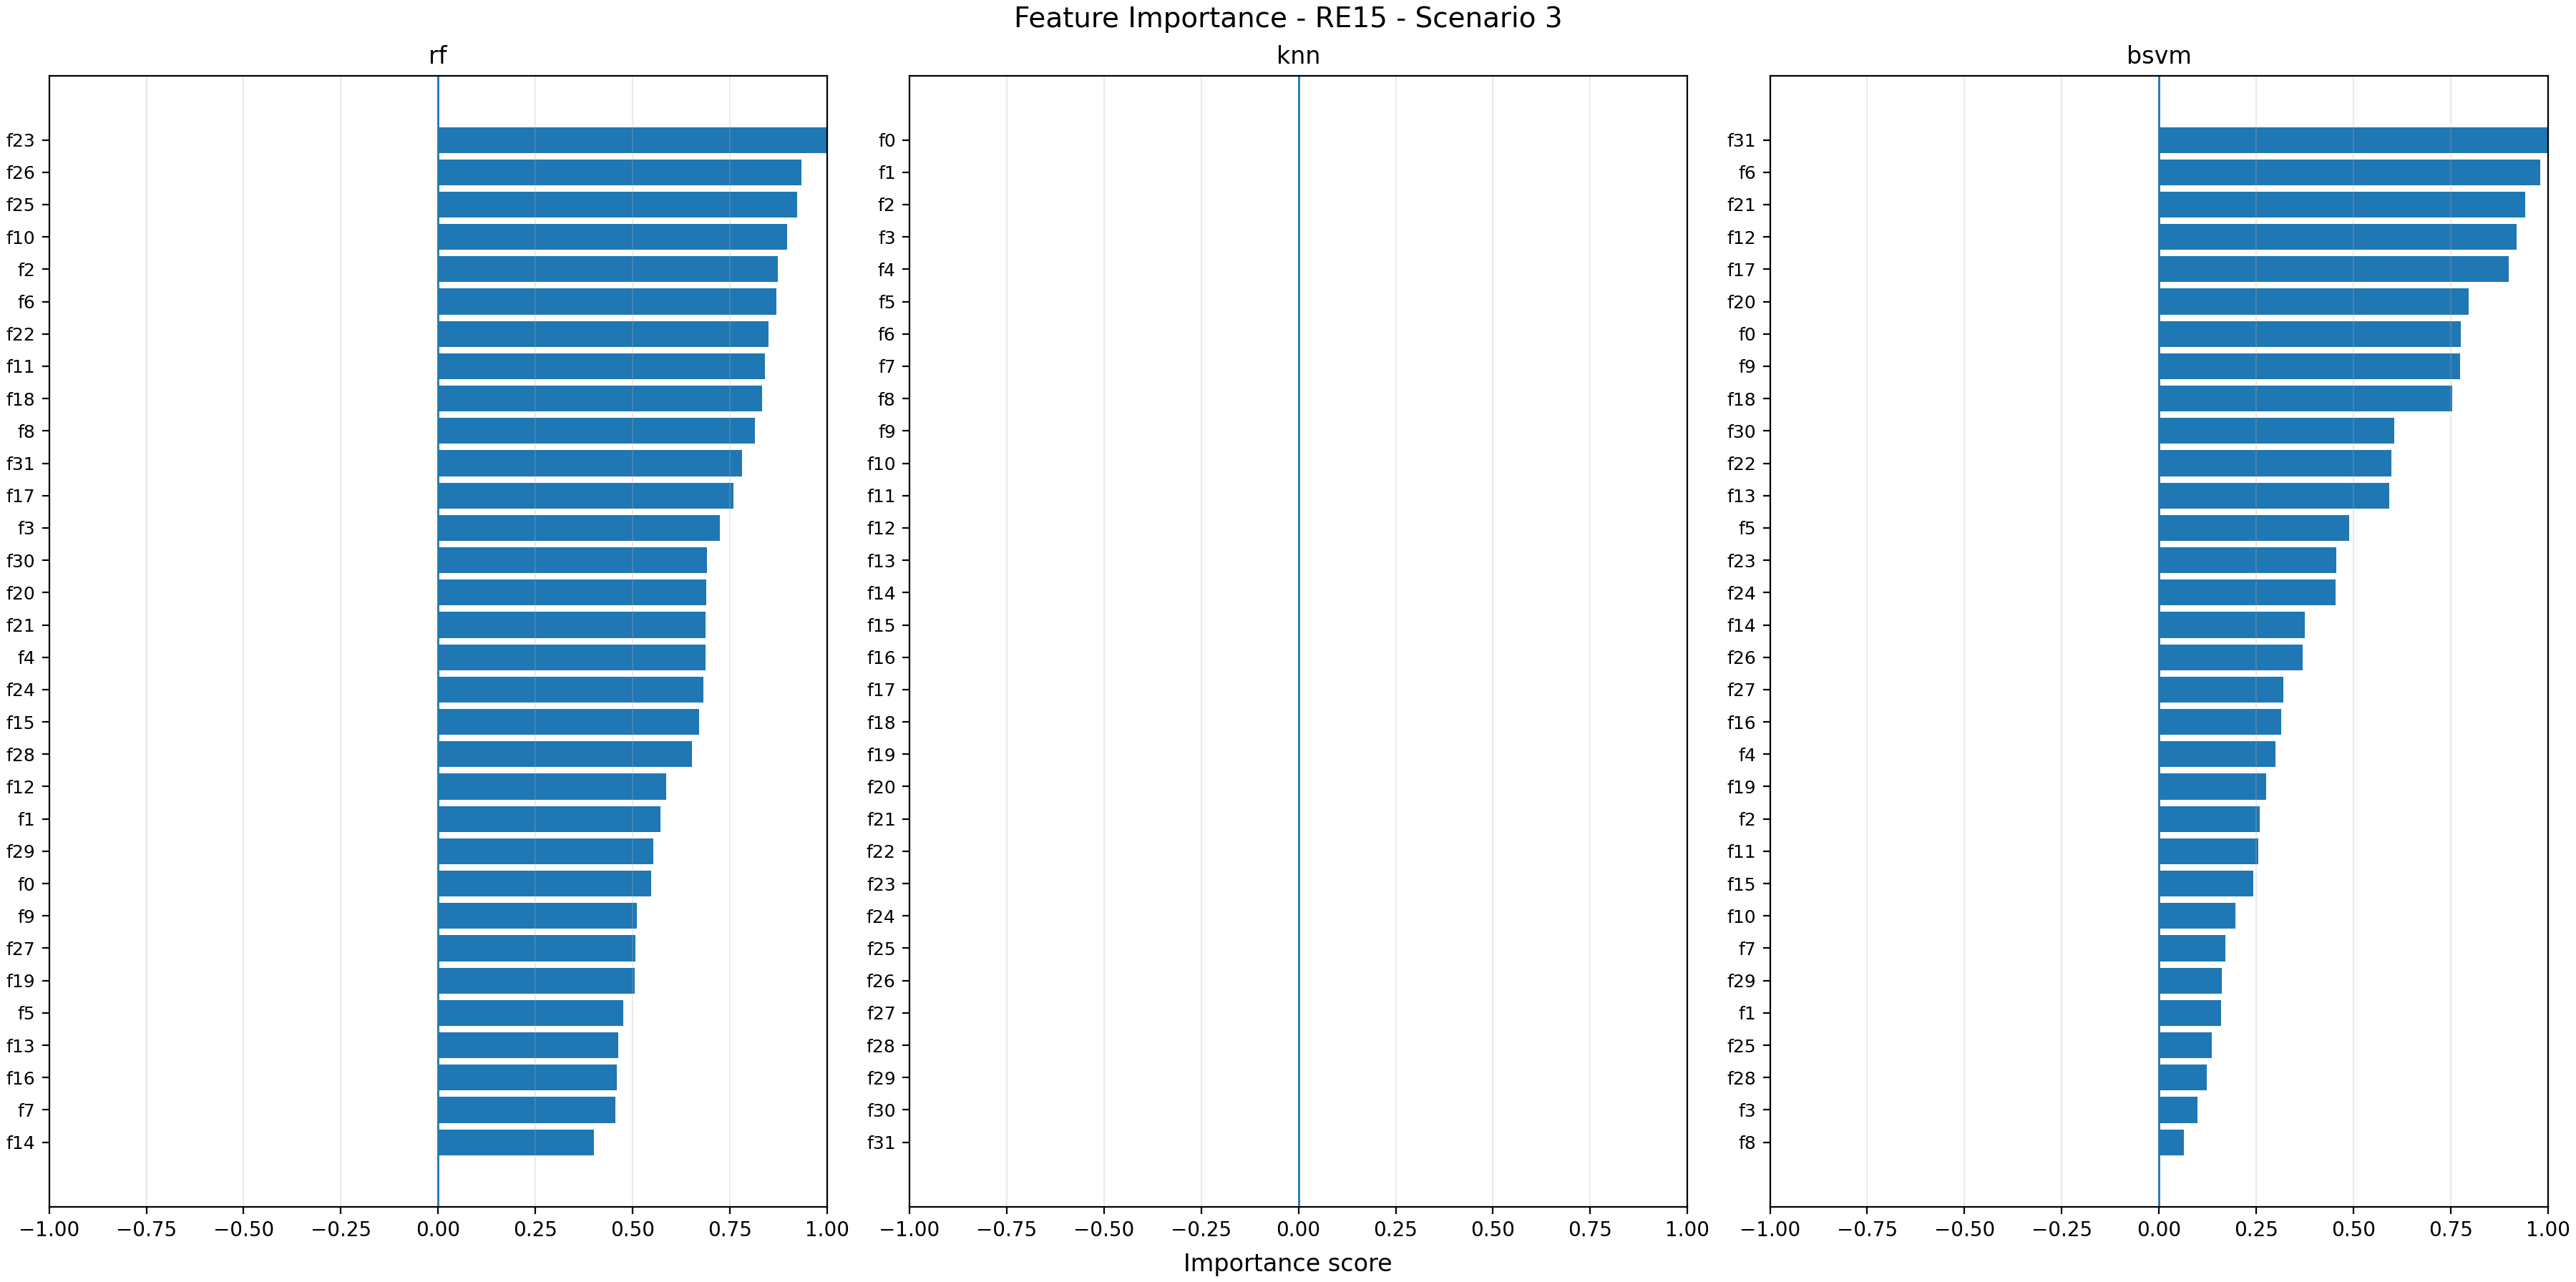
\includegraphics[width=\linewidth]{chapters/fi_helpful_panels_re15_s3.png}
	\caption{Feature Importance — RE15, Scenario 3}
	\label{fig:fi-re15-s3}
\end{figure}

In Scenario~3 under RE15 (\cref{fig:fi-re15-s3}),
the importance structure becomes considerably less distinctive.
\ac{KNN} assigns nearly uniform importance across features,
Random Forest distributes importance broadly without clear dominance,
and Binary \ac{SVM} concentrates on a small subset of higher-weight
components.

Overall, the RE15 representation yields less structured and less
consistent importance patterns than RAW, which aligns with the
observed degradation in classification performance.

\clearpage
\subsection{Venn Diagrams}

The Venn diagrams visualize the overlap of misclassified samples
between the three traditional \ac{ML} classifiers within each scenario.
Each circle represents the set of incorrectly classified instances
for one classifier. Pairwise intersections indicate samples that
are misclassified by two classifiers, while the triple intersection
represents instances that are misclassified by all three models.
Large overlap regions therefore indicate agreement in error behavior,
whereas large regions without overlaps reveal classifier-specific weaknesses.

\begin{figure}[!htbp]
    \centering
    \begin{subfigure}[t]{0.32\linewidth}
        \centering
        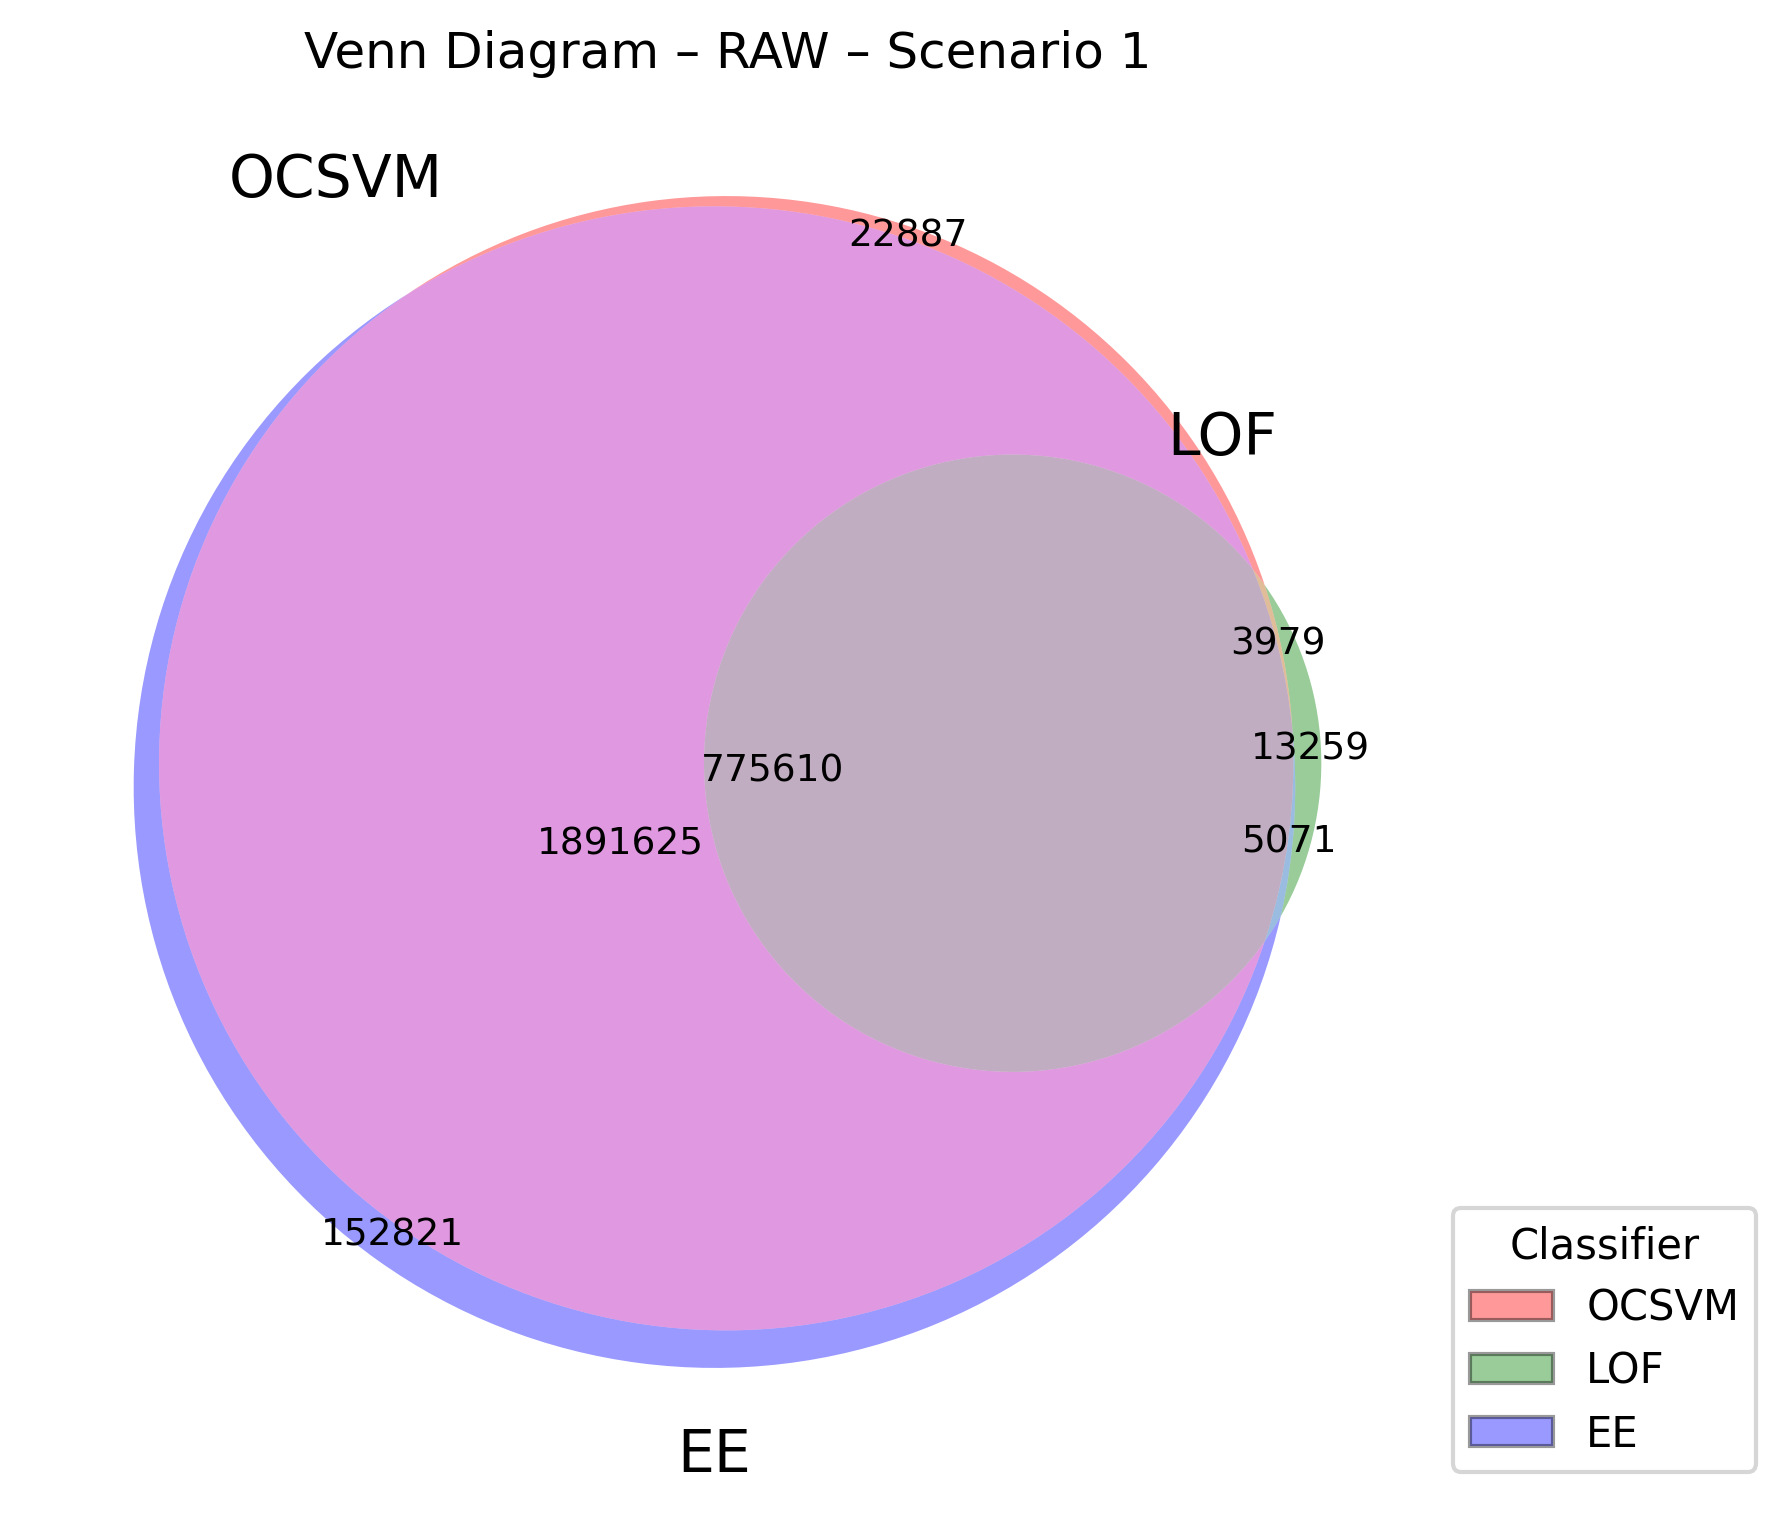
\includegraphics[width=\linewidth]{chapters/venn_raw_s1.png}
        \caption{Scenario 1}
    \end{subfigure}\hfill
    \begin{subfigure}[t]{0.32\linewidth}
        \centering
        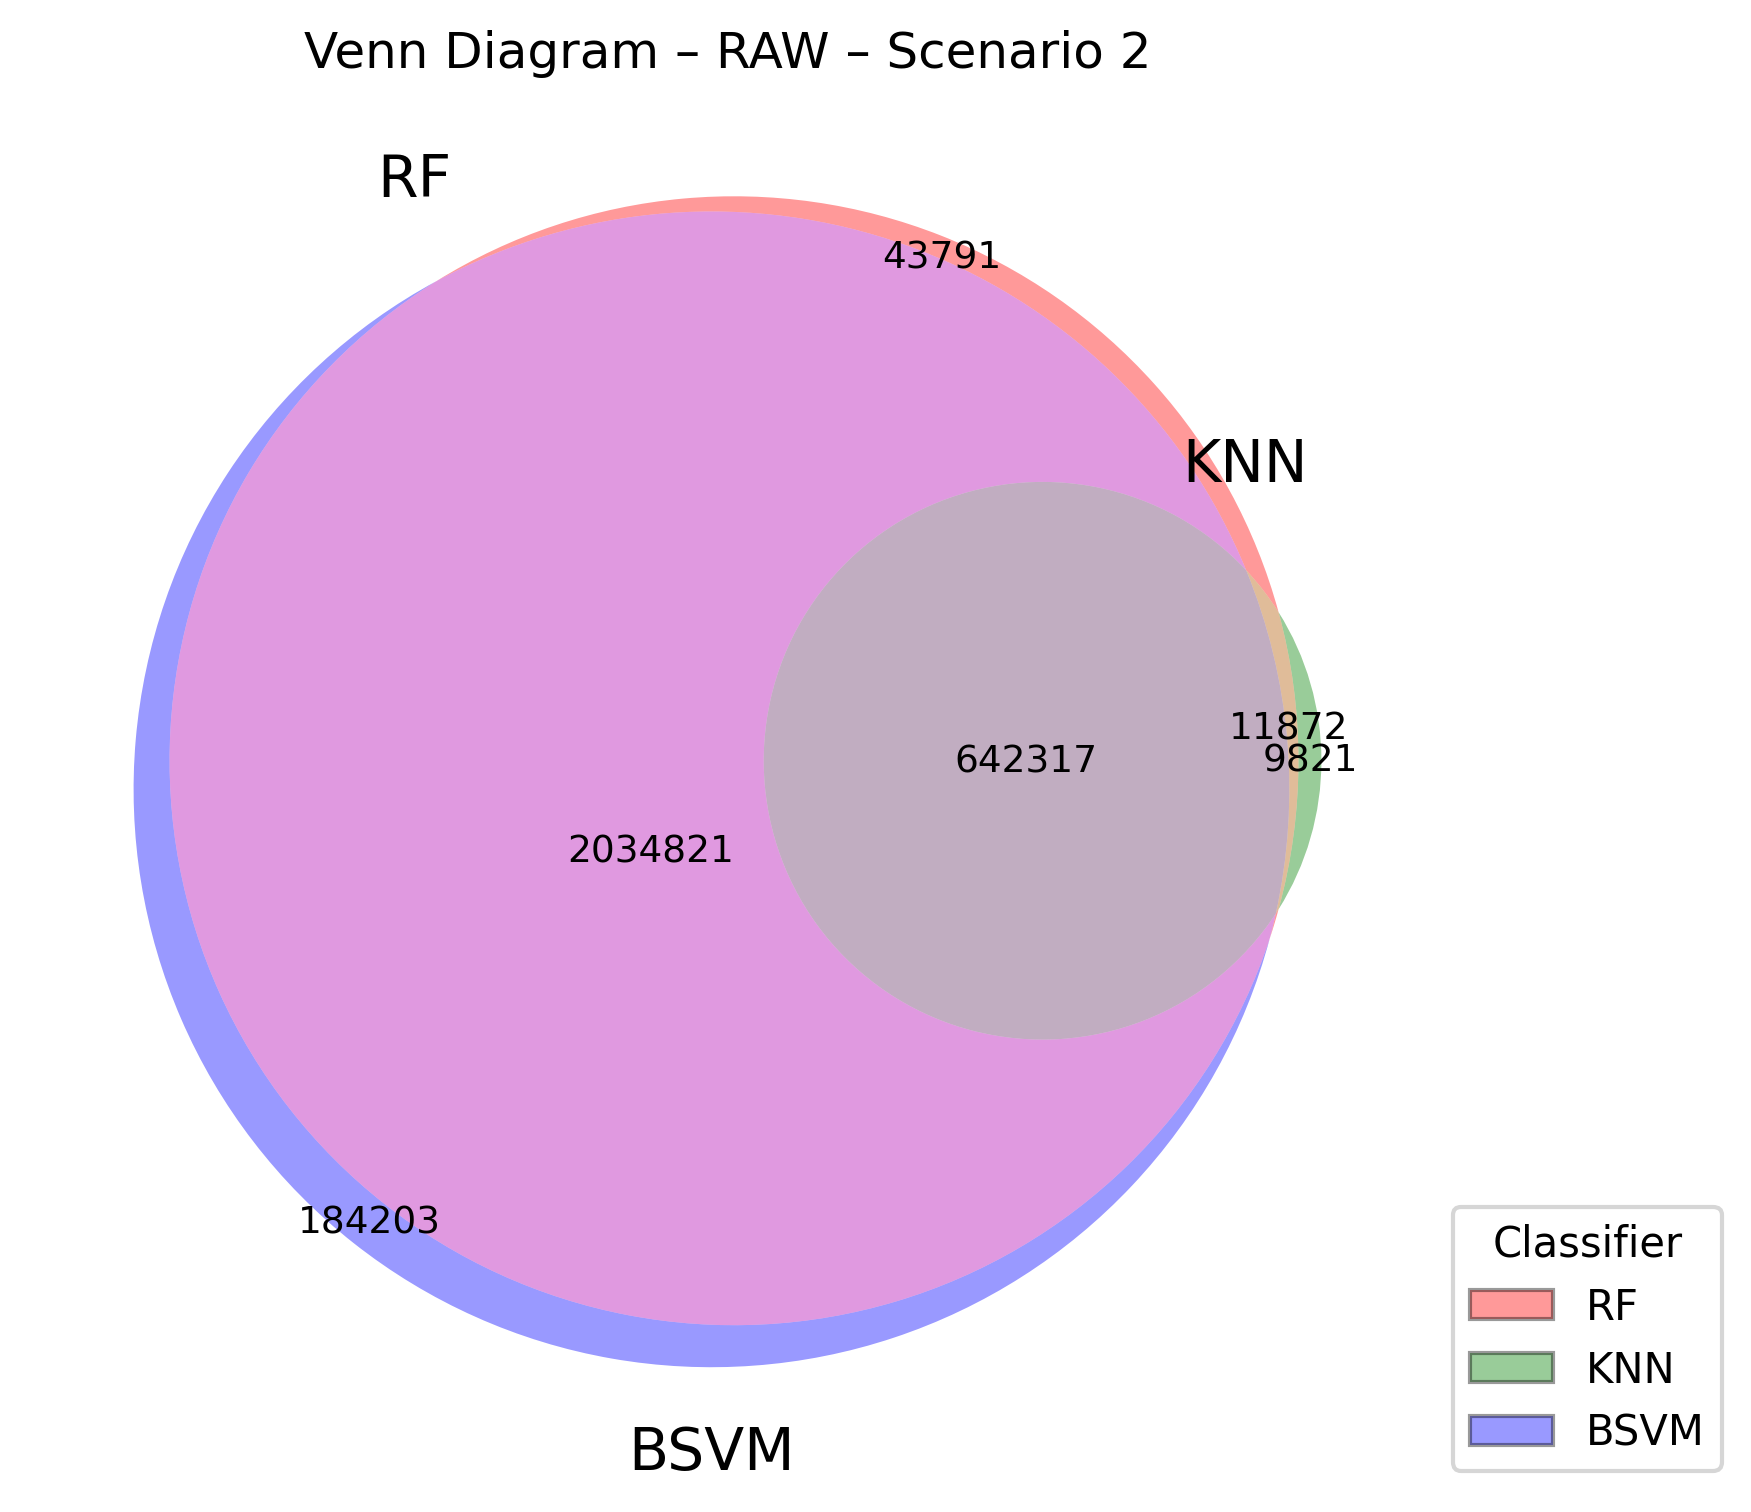
\includegraphics[width=\linewidth]{chapters/venn_raw_s2.png}
        \caption{Scenario 2}
    \end{subfigure}\hfill
    \begin{subfigure}[t]{0.32\linewidth}
        \centering
        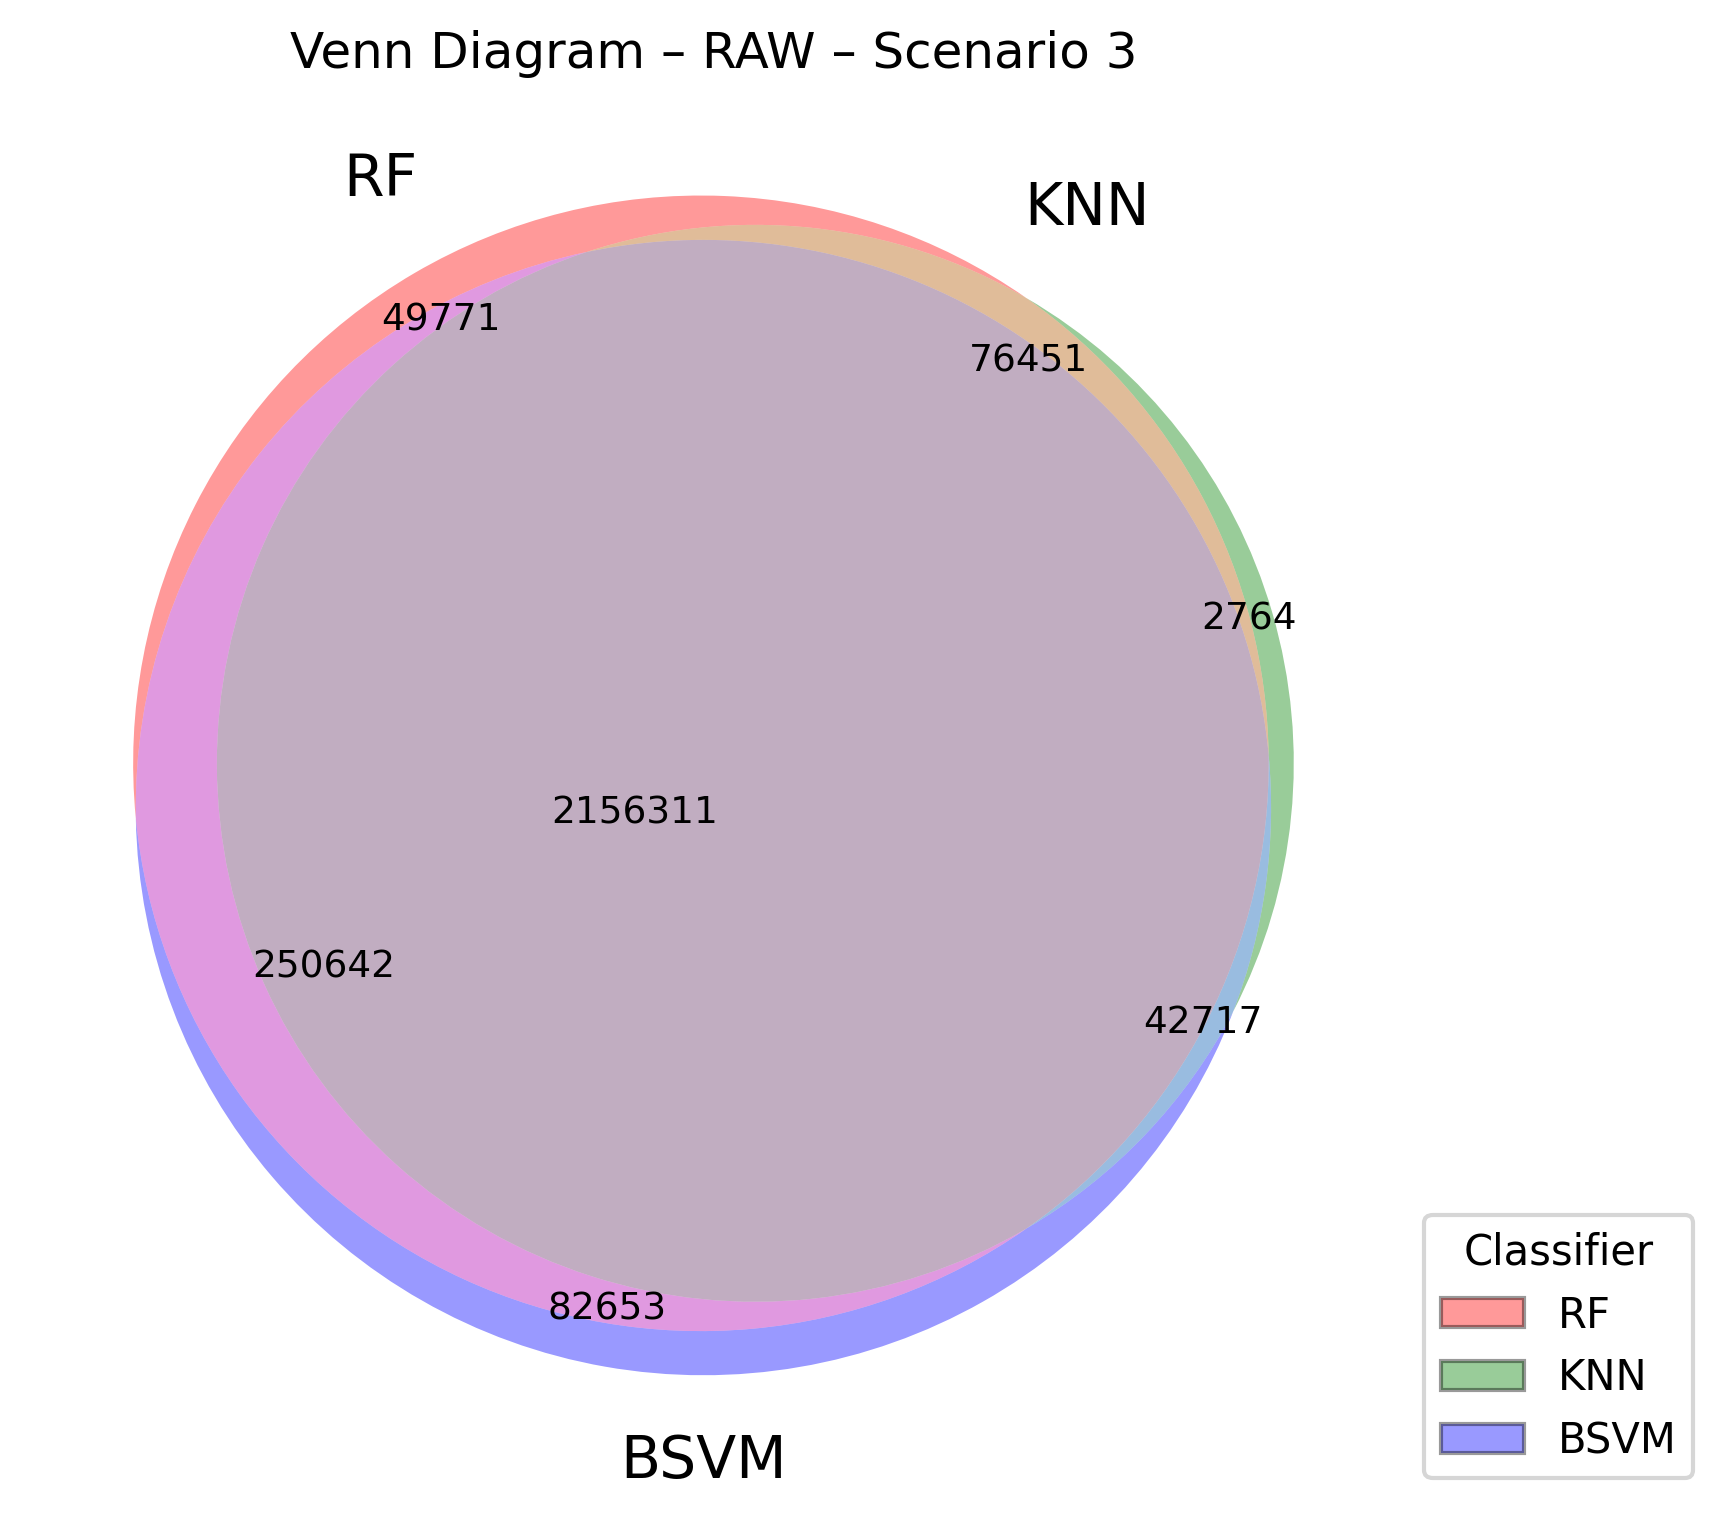
\includegraphics[width=\linewidth]{chapters/venn_raw_s3.png}
        \caption{Scenario 3}
    \end{subfigure}
    \caption{Error overlaps (Venn diagrams) for the RAW representation.}
    \label{fig:venn-raw}
\end{figure}

\paragraph{RAW Representation}

For the RAW dataset, the absolute number of errors is substantially
higher due to the larger number of evaluated samples. As \cref{fig:venn-raw} shows in Scenarios~1
and~2, the diagrams are dominated by large pairwise overlaps.
In particular, OCSVM and EE (Scenario~1) as well as RF and Binary SVM
(Scenario~2) exhibit highly similar error patterns. This suggests that
these classifier pairs learn comparable decision boundaries when using
RAW packet features, while the third classifier contributes only a
limited amount of additional unique errors.

In Scenario~3 (RAW), the triple intersection becomes the dominant
region. Most misclassified instances are shared across all classifiers,
indicating that errors are not model-specific but correspond to a
common subset of intrinsically difficult samples. This observation
explains why ensemble aggregation provides only limited improvement
in this scenario: when all base classifiers fail on the same instances,
the ensemble cannot compensate.

\begin{figure}[!htbp]
    \centering
    \begin{subfigure}[t]{0.32\linewidth}
        \centering
        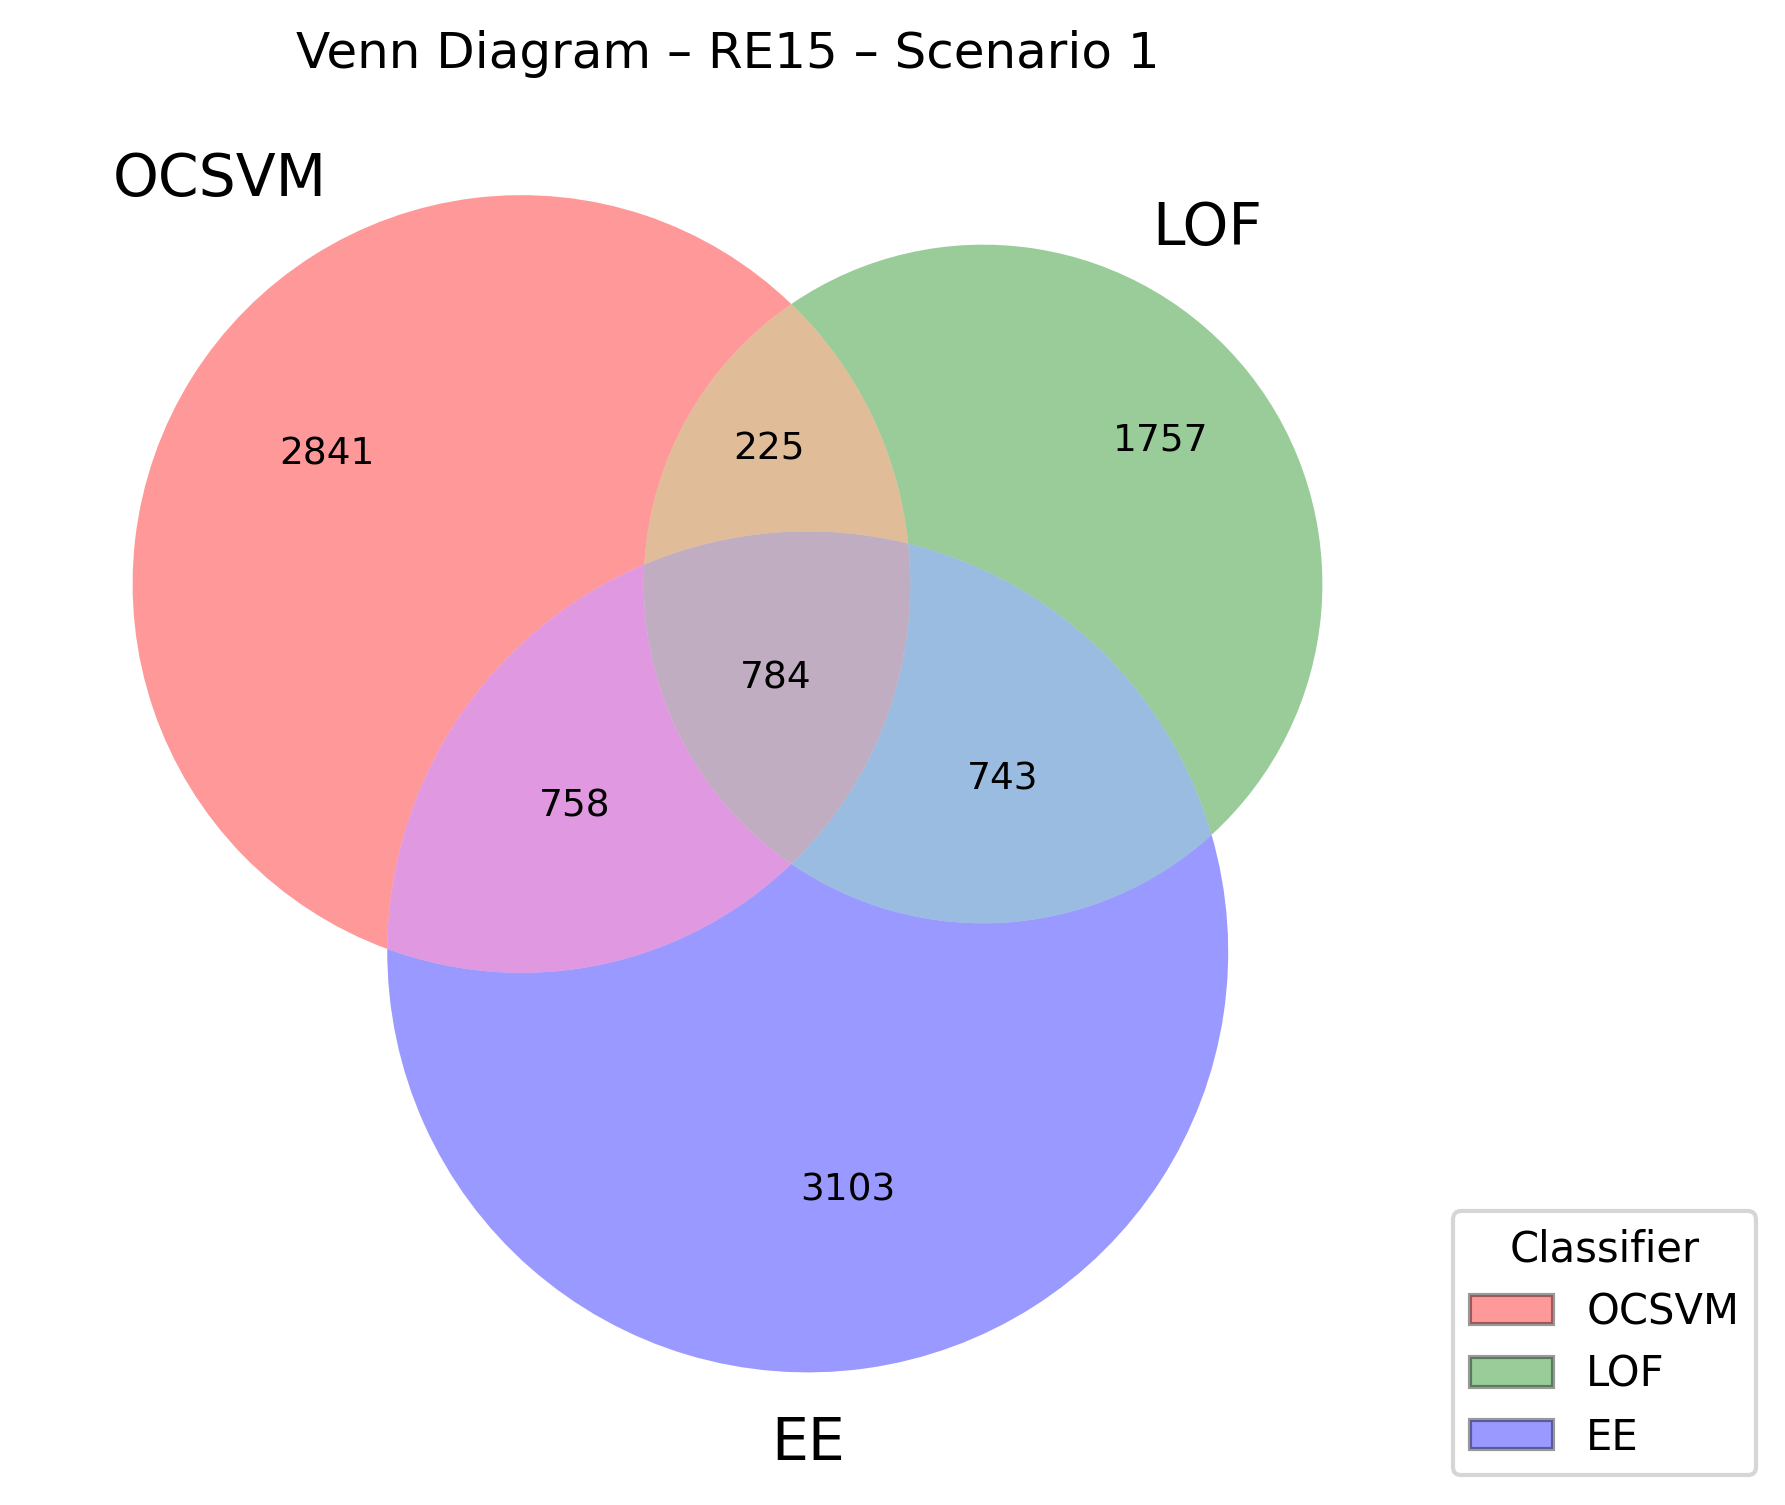
\includegraphics[width=\linewidth]{chapters/venn_re15_s1.png}
        \caption{Scenario 1}
    \end{subfigure}\hfill
    \begin{subfigure}[t]{0.32\linewidth}
        \centering
        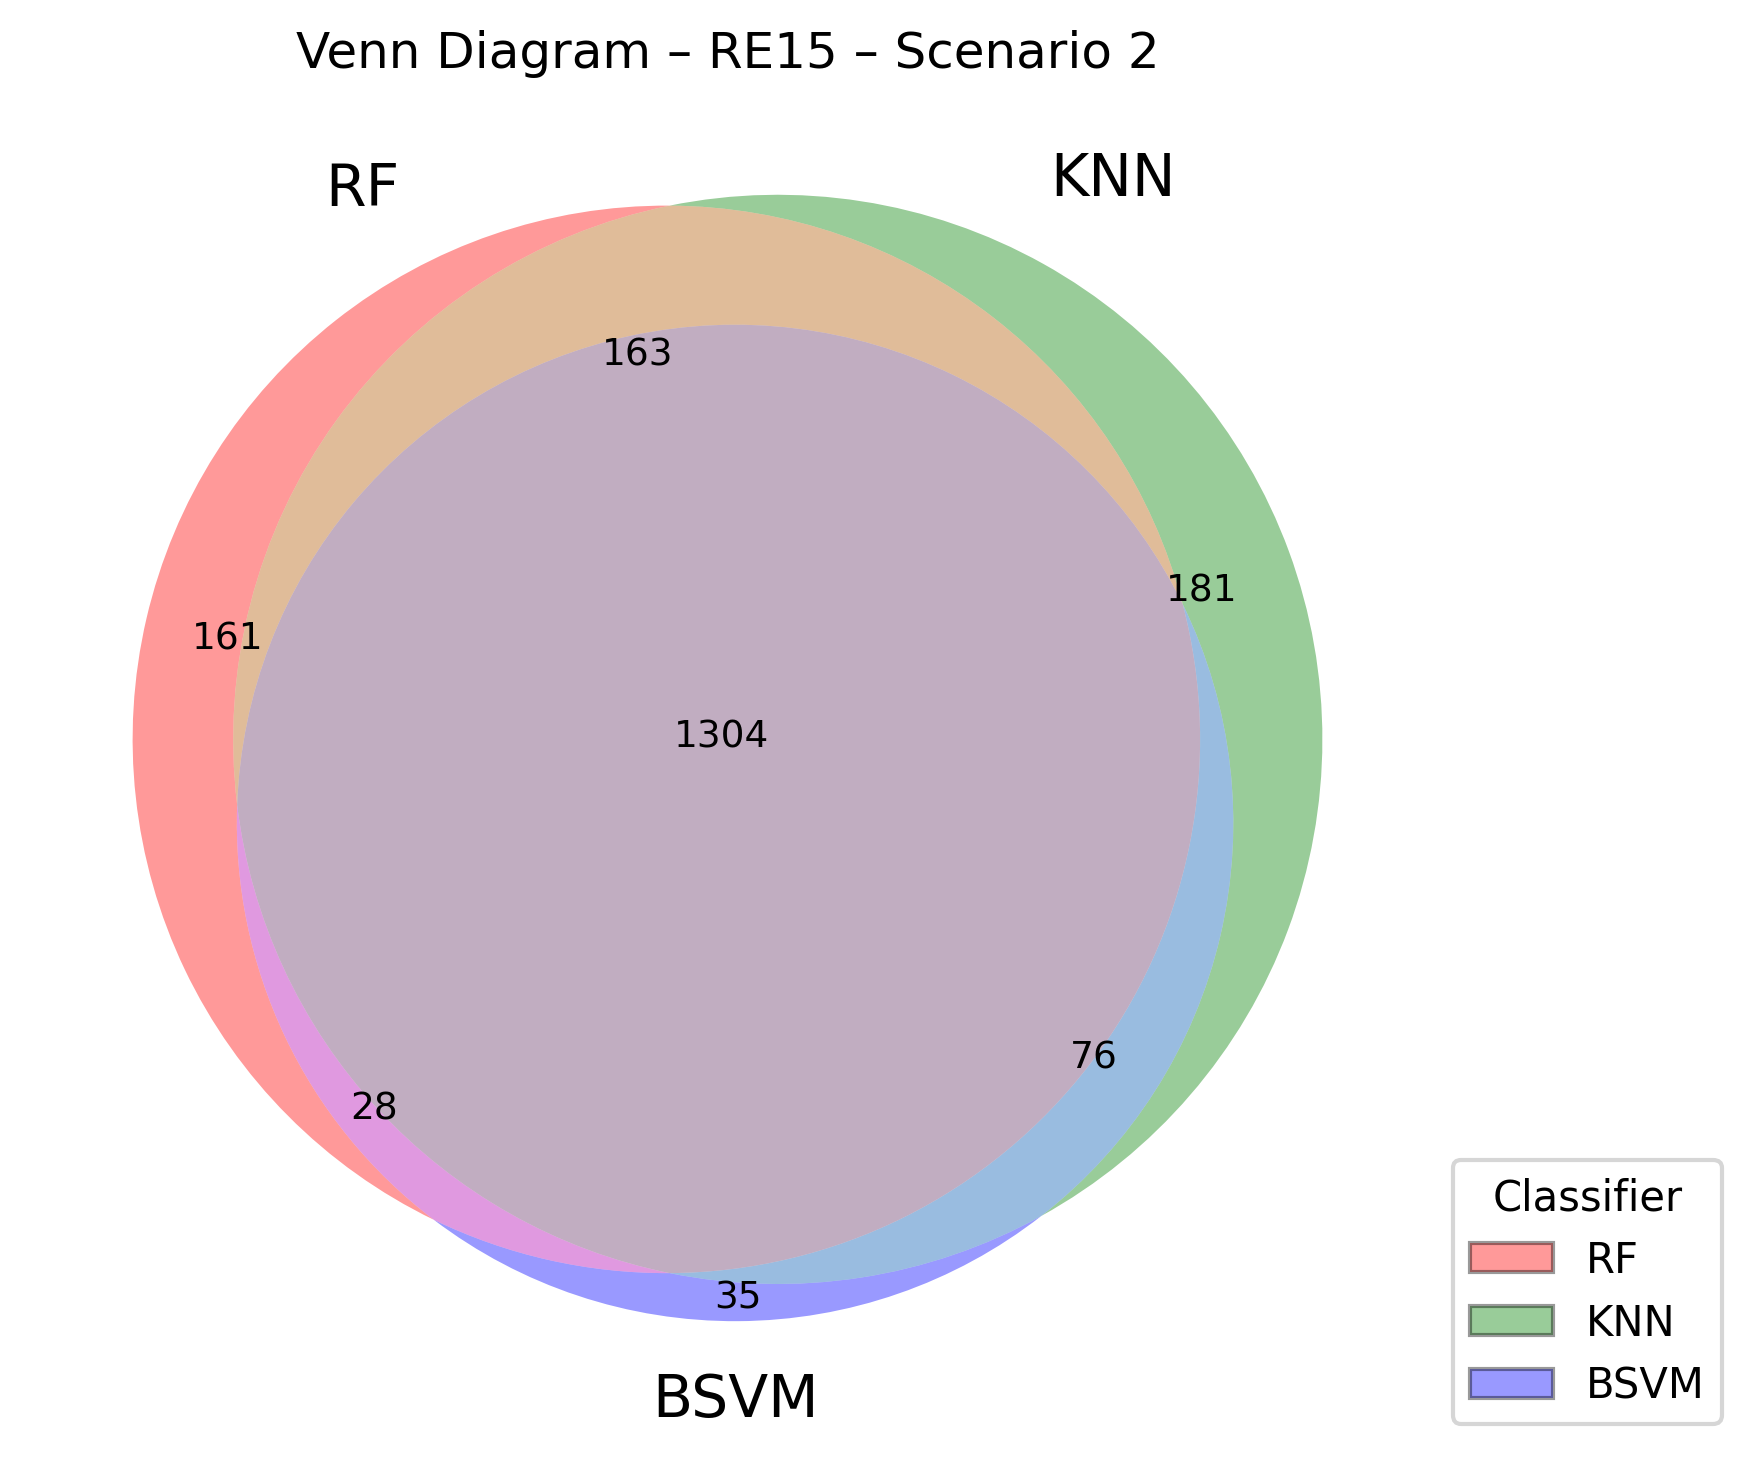
\includegraphics[width=\linewidth]{chapters/venn_re15_s2.png}
        \caption{Scenario 2}
    \end{subfigure}\hfill
    \begin{subfigure}[t]{0.32\linewidth}
        \centering
        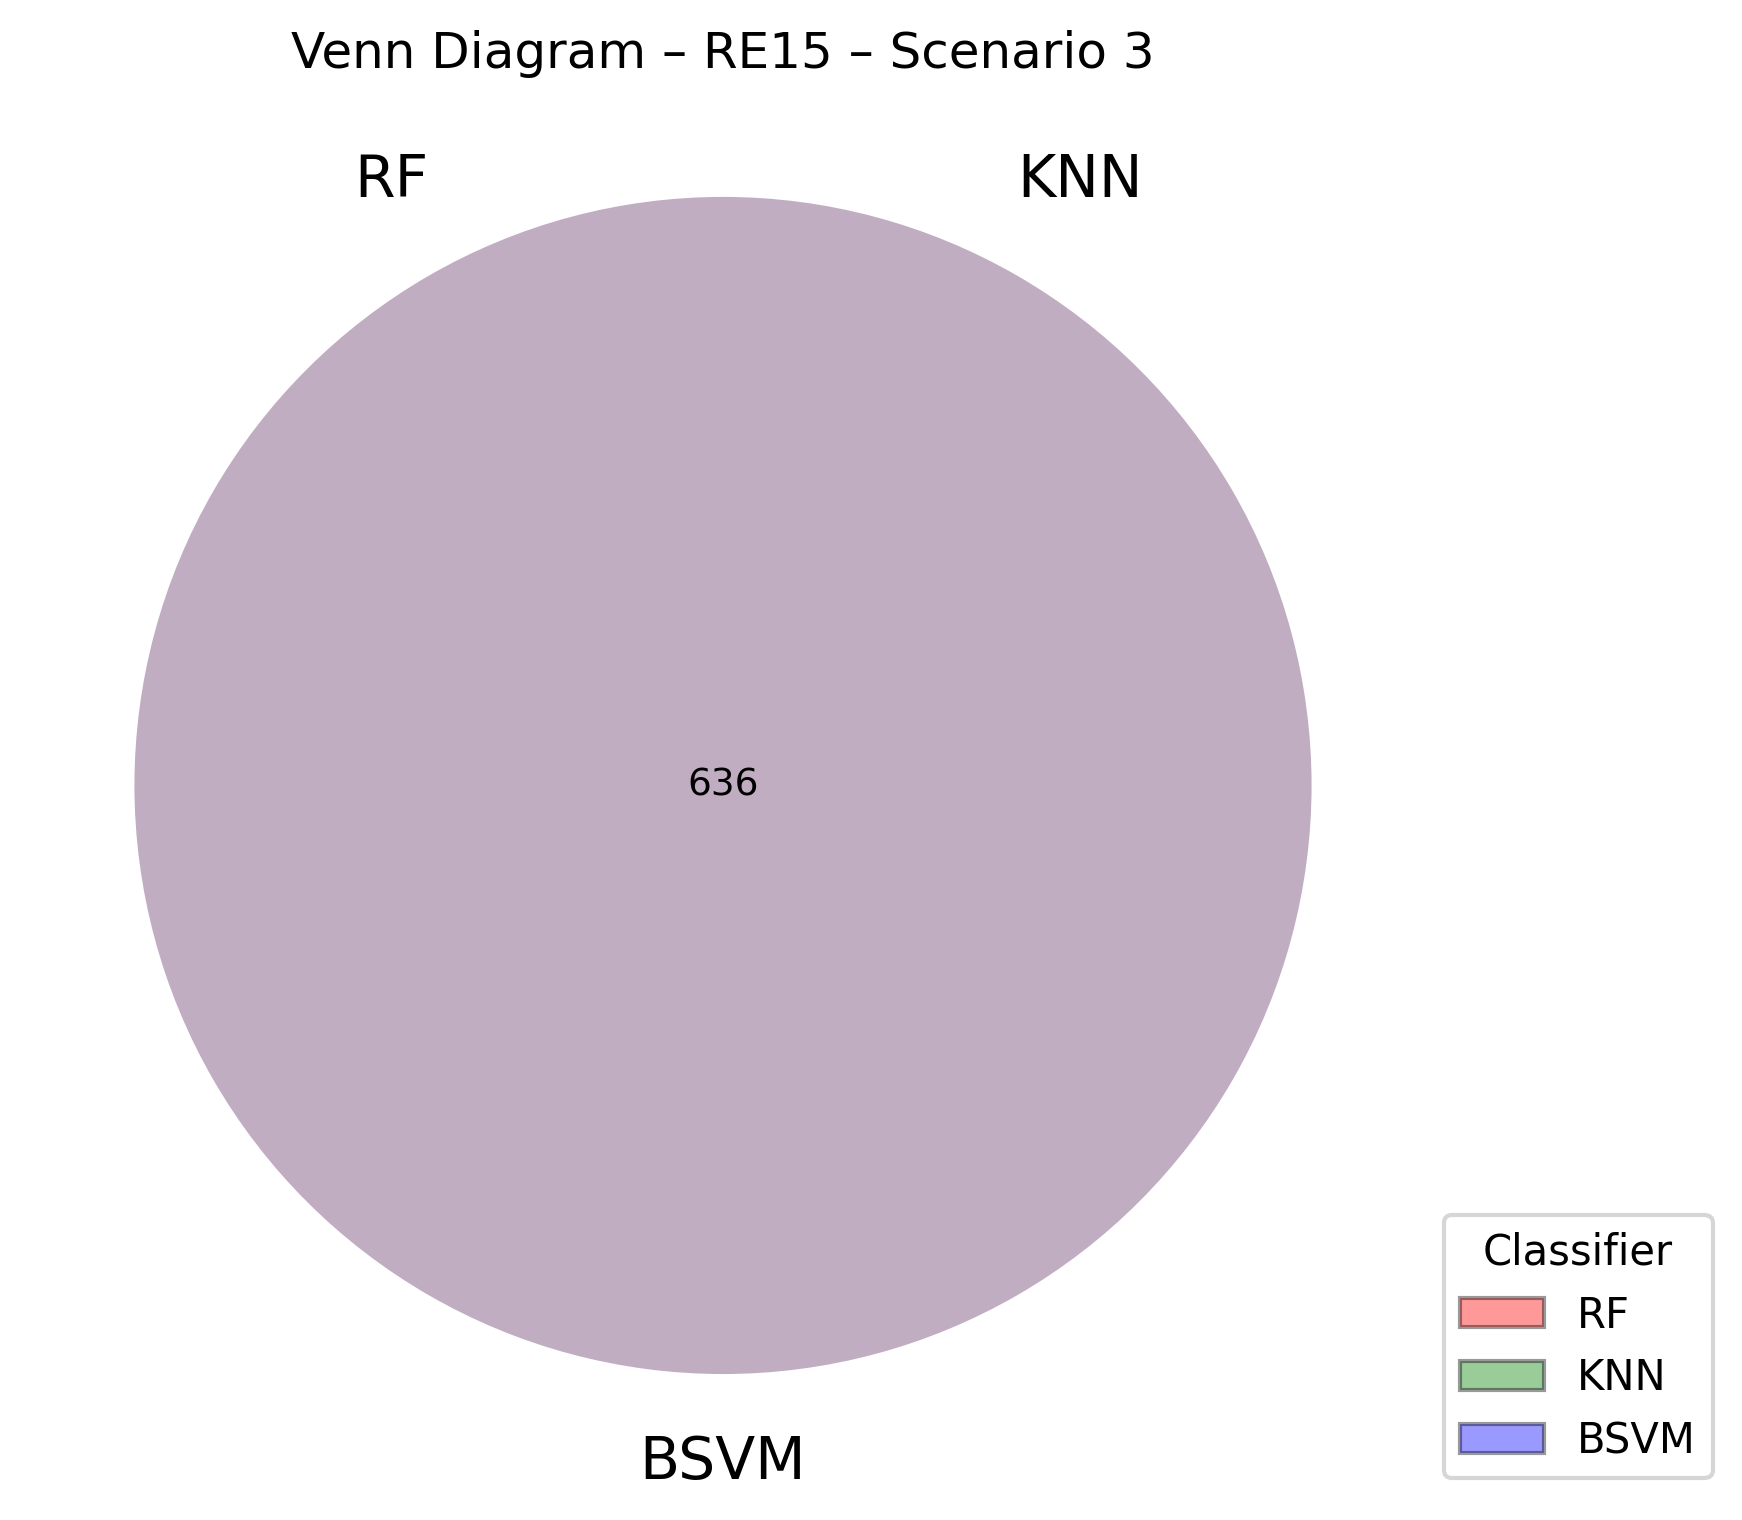
\includegraphics[width=\linewidth]{chapters/venn_re15_s3.png}
        \caption{Scenario 3}
    \end{subfigure}
    \caption{Error overlaps (Venn diagrams) for the RE15 representation.}
    \label{fig:venn-re15}
\end{figure}

\paragraph{RE15 Representation}

For the RE15 representation, the overlap structure changes across
scenarios. In Scenario~1, the diagrams show considerable classifier-
specific error regions (\cref{fig:venn-re15}), meaning that each model misclassifies a
substantial number of samples that the others classify correctly.
Although a triple overlap exists, it is not dominant, indicating
divergent decision behavior.

In Scenario~2, the triple intersection becomes the largest region,
while the unique error regions shrink considerably. This indicates
that most misclassifications are shared among all classifiers,
and only a small fraction depends on the model choice.

In Scenario~3, the triple overlap effectively covers the entire
error set. All three classifiers misclassify the same instances,
representing complete agreement in failure cases. Under this
condition, the ensemble classifier cannot improve performance,
since altering the aggregation strategy does not change the
underlying error set.

%{\color{gray} \paragraph{Relation to Ensemble Performance}
%The overlap analysis clarifies the ensemble results observed earlier.
%When classifier errors strongly overlap (large triple intersections),
%ensemble aggregation offers limited gains, as shared errors cannot
%be corrected. Conversely, scenarios with larger classifier-specific
%regions provide more potential for ensemble improvements, since
%disagreement between models allows majority voting or random
%selection to mitigate individual weaknesses.}

\clearpage
\subsection{Runtime and Memory Consumption}
\subsubsection{Runtime}
\begin{figure}[!htbp]
	\centering
	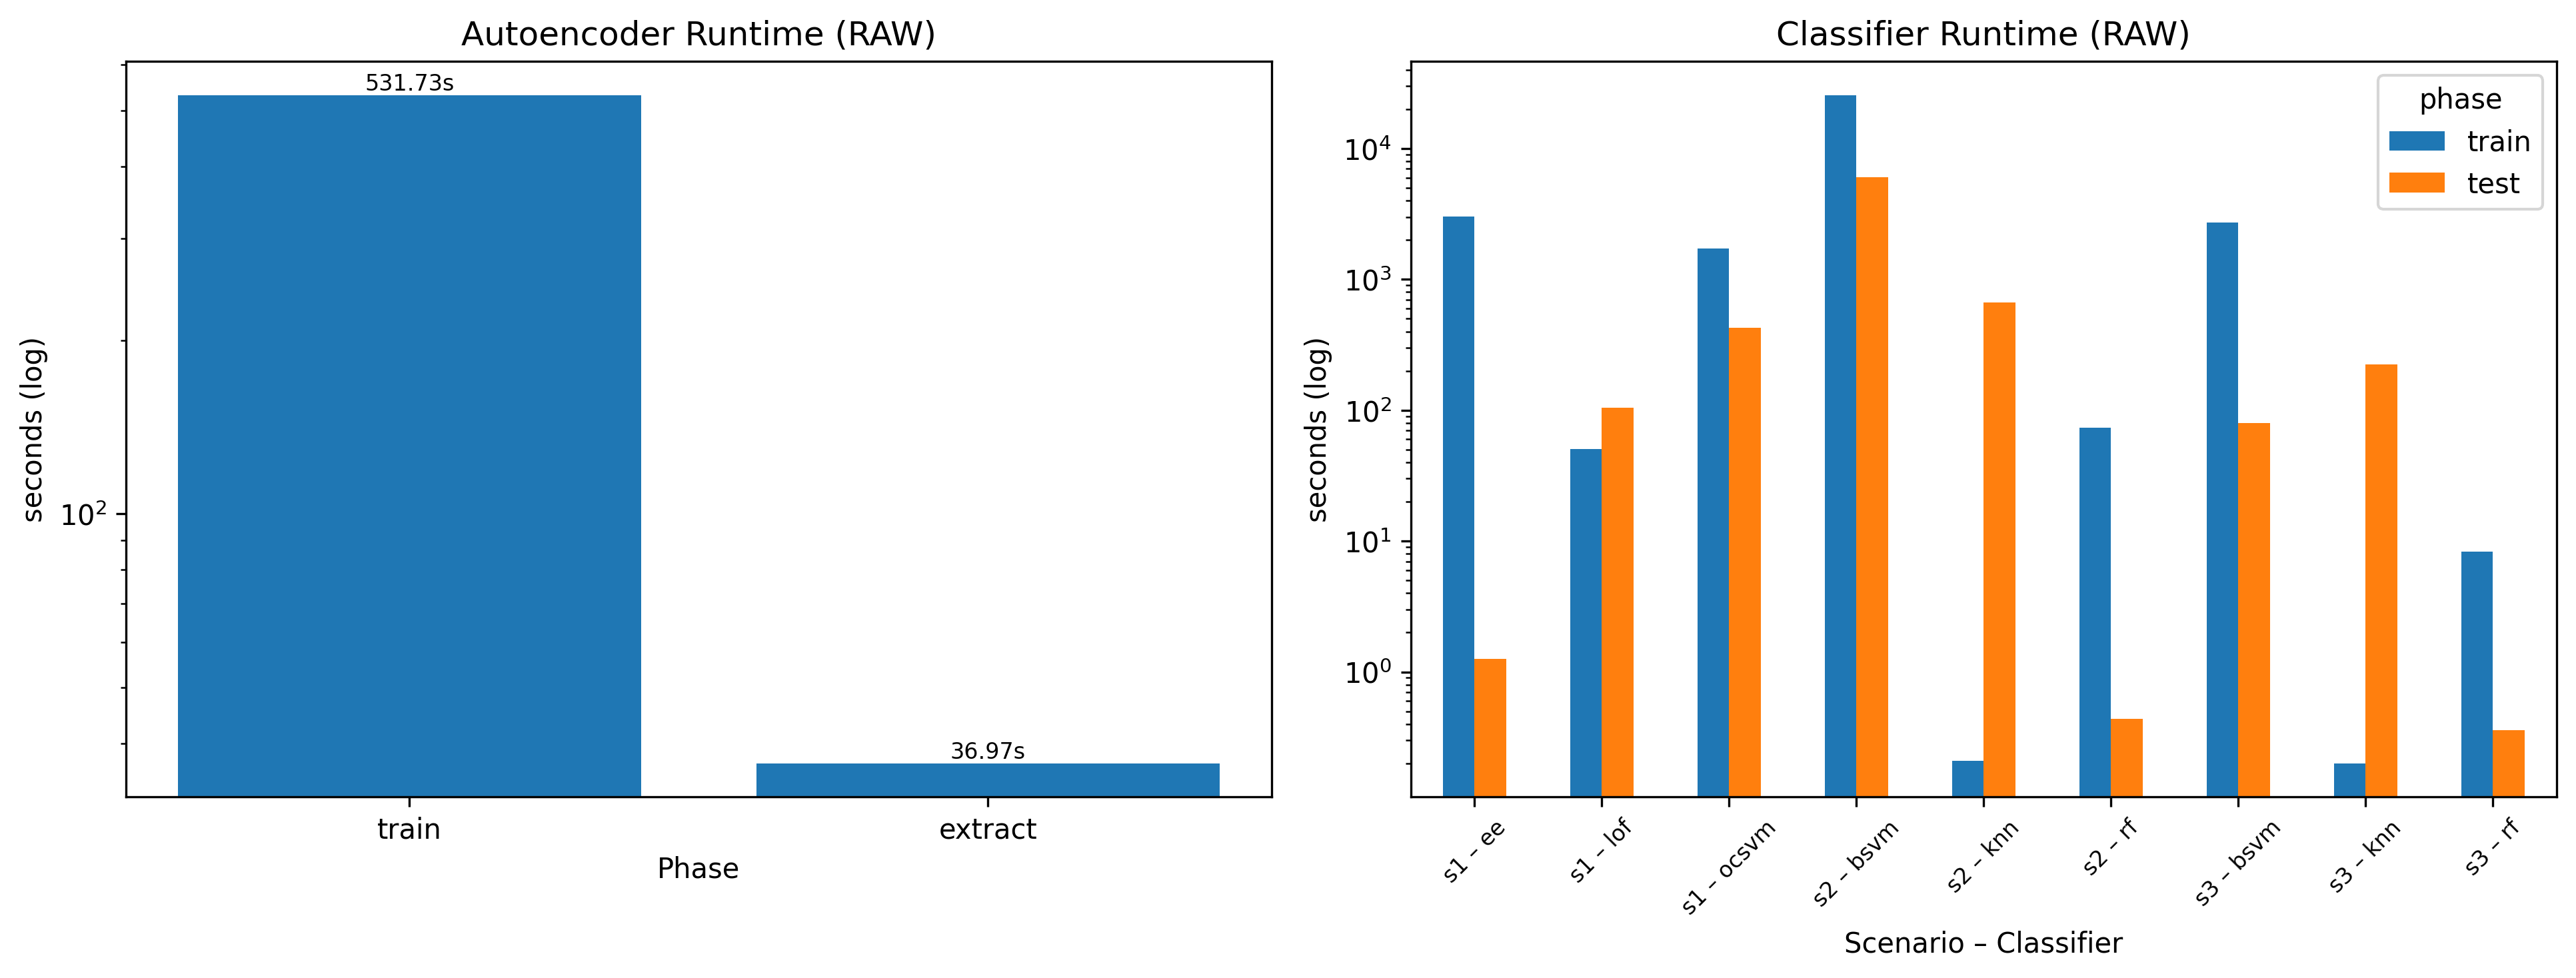
\includegraphics[width=\linewidth]{chapters/runtime_raw.png}
	\caption{Runtime of Feature Extraction and Traditional \ac{ML} Models — RAW}
	\label{fig:runtime-raw}
\end{figure}

For the RAW representation (\cref{fig:runtime-raw}), classifier
runtimes vary drastically across models and scenarios.
In general, training requires more time than testing; however,
important exceptions exist.

Binary \ac{SVM} exhibits the highest computational cost, particularly
in Scenario~2, where both training and testing times are extremely
large. Elliptic Envelope and \ac{OCSVM} also incur substantial training
costs in Scenario~1. In contrast, \ac{KNN} has an almost negligible
training time, as it merely stores the training data. Its prediction
phase, however, is significantly more expensive because each test
instance requires distance computations to many stored samples.
This asymmetry is especially pronounced for RAW features.

Random Forest achieves comparatively small testing times,
particularly in Scenarios~2 and~3, where predictions are performed
in sub-second ranges. Overall, for RAW features the classifier
choice strongly influences total runtime, with \ac{SVM}-based models
and \ac{KNN} representing the main computational bottlenecks.

\begin{figure}[!htbp]
	\centering
	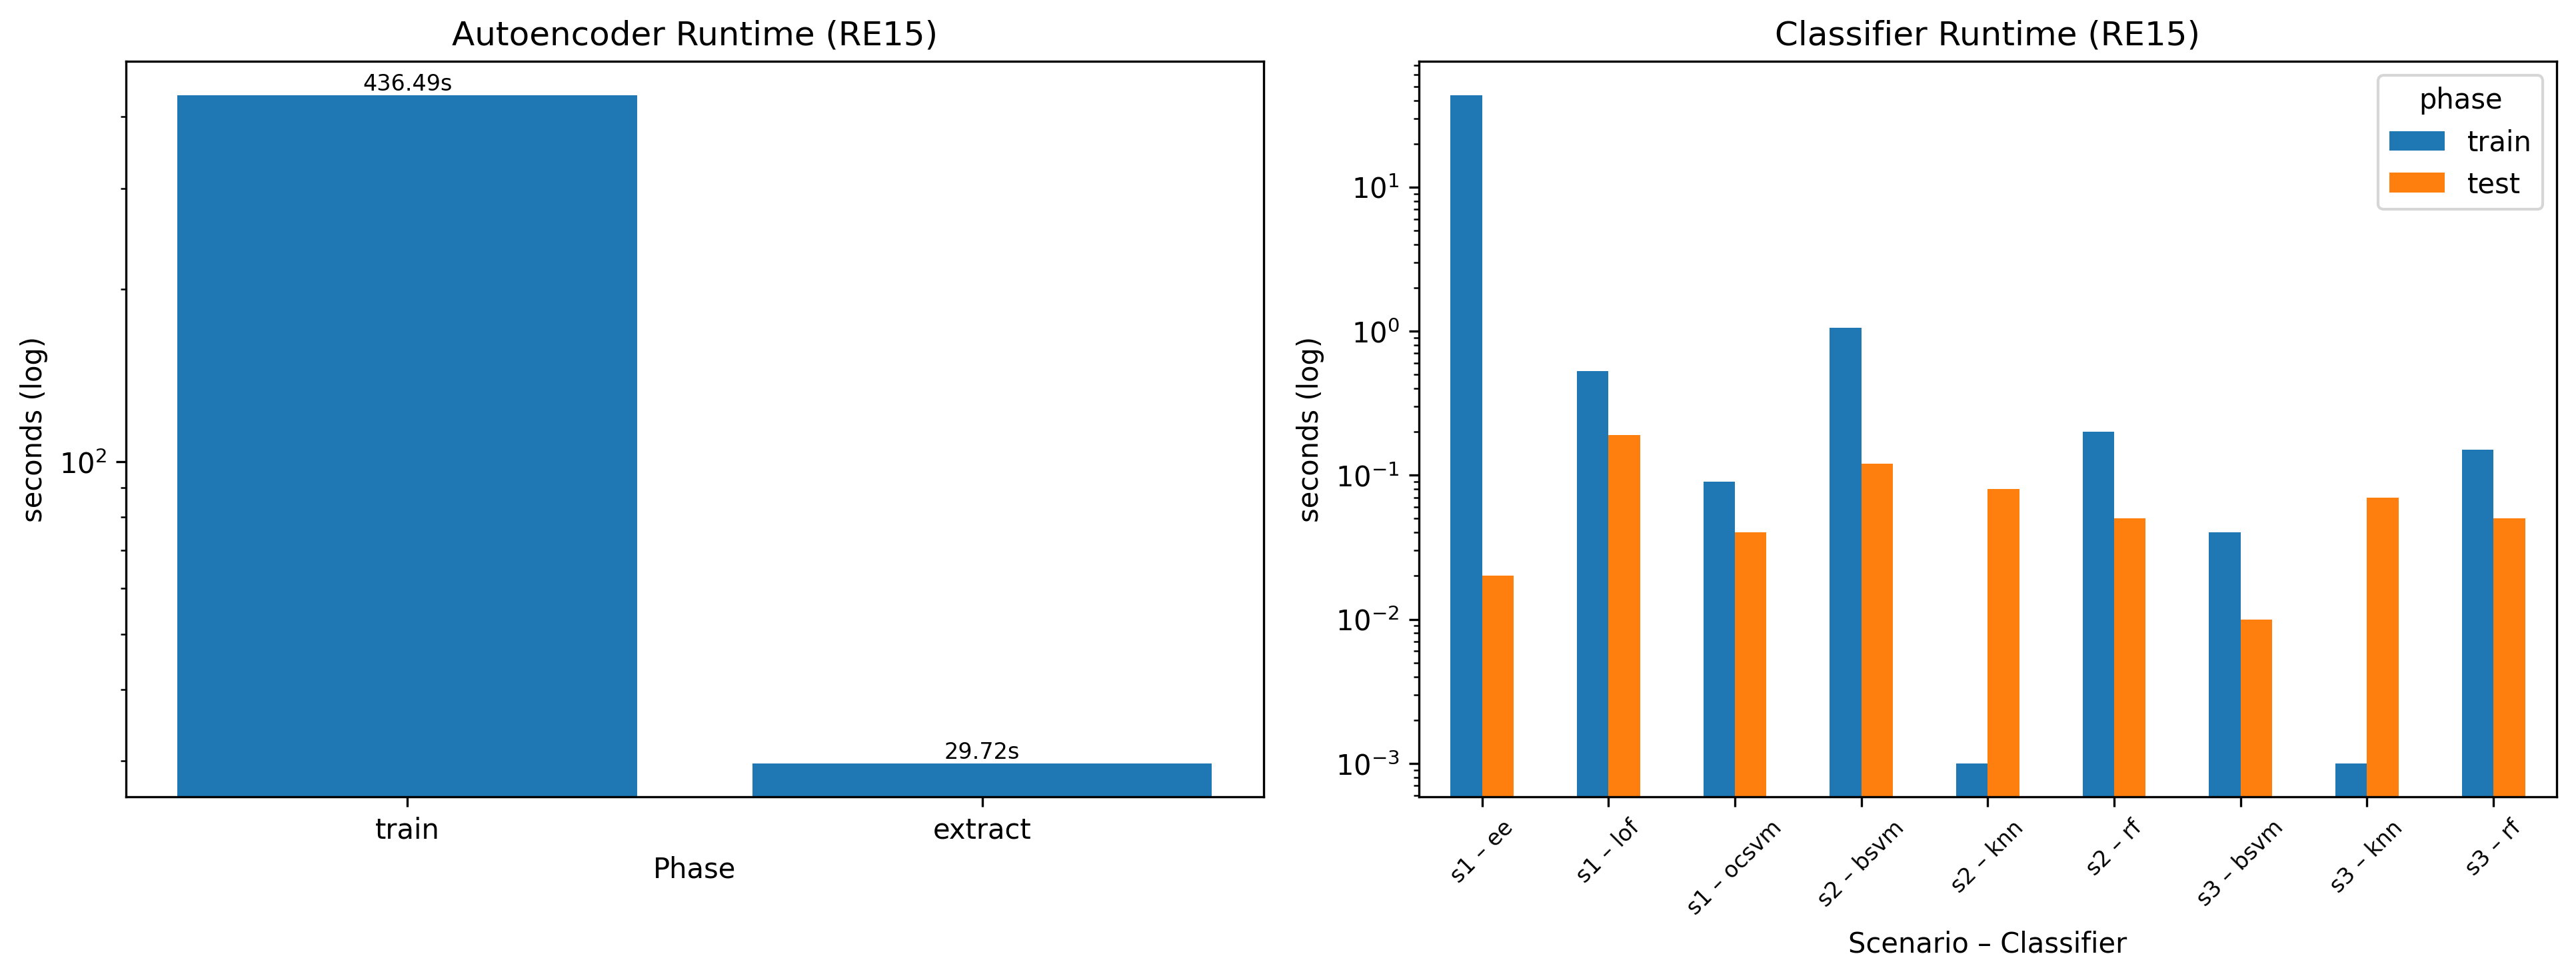
\includegraphics[width=\linewidth]{chapters/runtime_re15.png}
	\caption{Runtime of Feature Extraction and Traditional ML Models — RE15}
	\label{fig:runtime-re15}
\end{figure}

When using the RE15 representation (\cref{fig:runtime-re15}),
classifier runtimes decrease dramatically.
Except for Elliptic Envelope, whose training time remains
noticeably higher than the others, most classifiers operate
within sub-second to approximately one-second ranges during
training. Testing times are consistently small and relatively
similar across models.

In this setting, the classifier stage is no longer the dominant
cost factor. Instead, the primary computational overhead stems
from the feature extraction step (autoencoder training),
while the subsequent classification becomes comparatively
lightweight.

Overall, the results indicate that RAW representations impose
significant computational demands at the classifier level,
whereas RE15 substantially reduces classifier runtime,
shifting the computational burden primarily to feature
extraction.

\subsubsection{Memory Consumption}

\begin{figure}[!htbp]
	\centering
	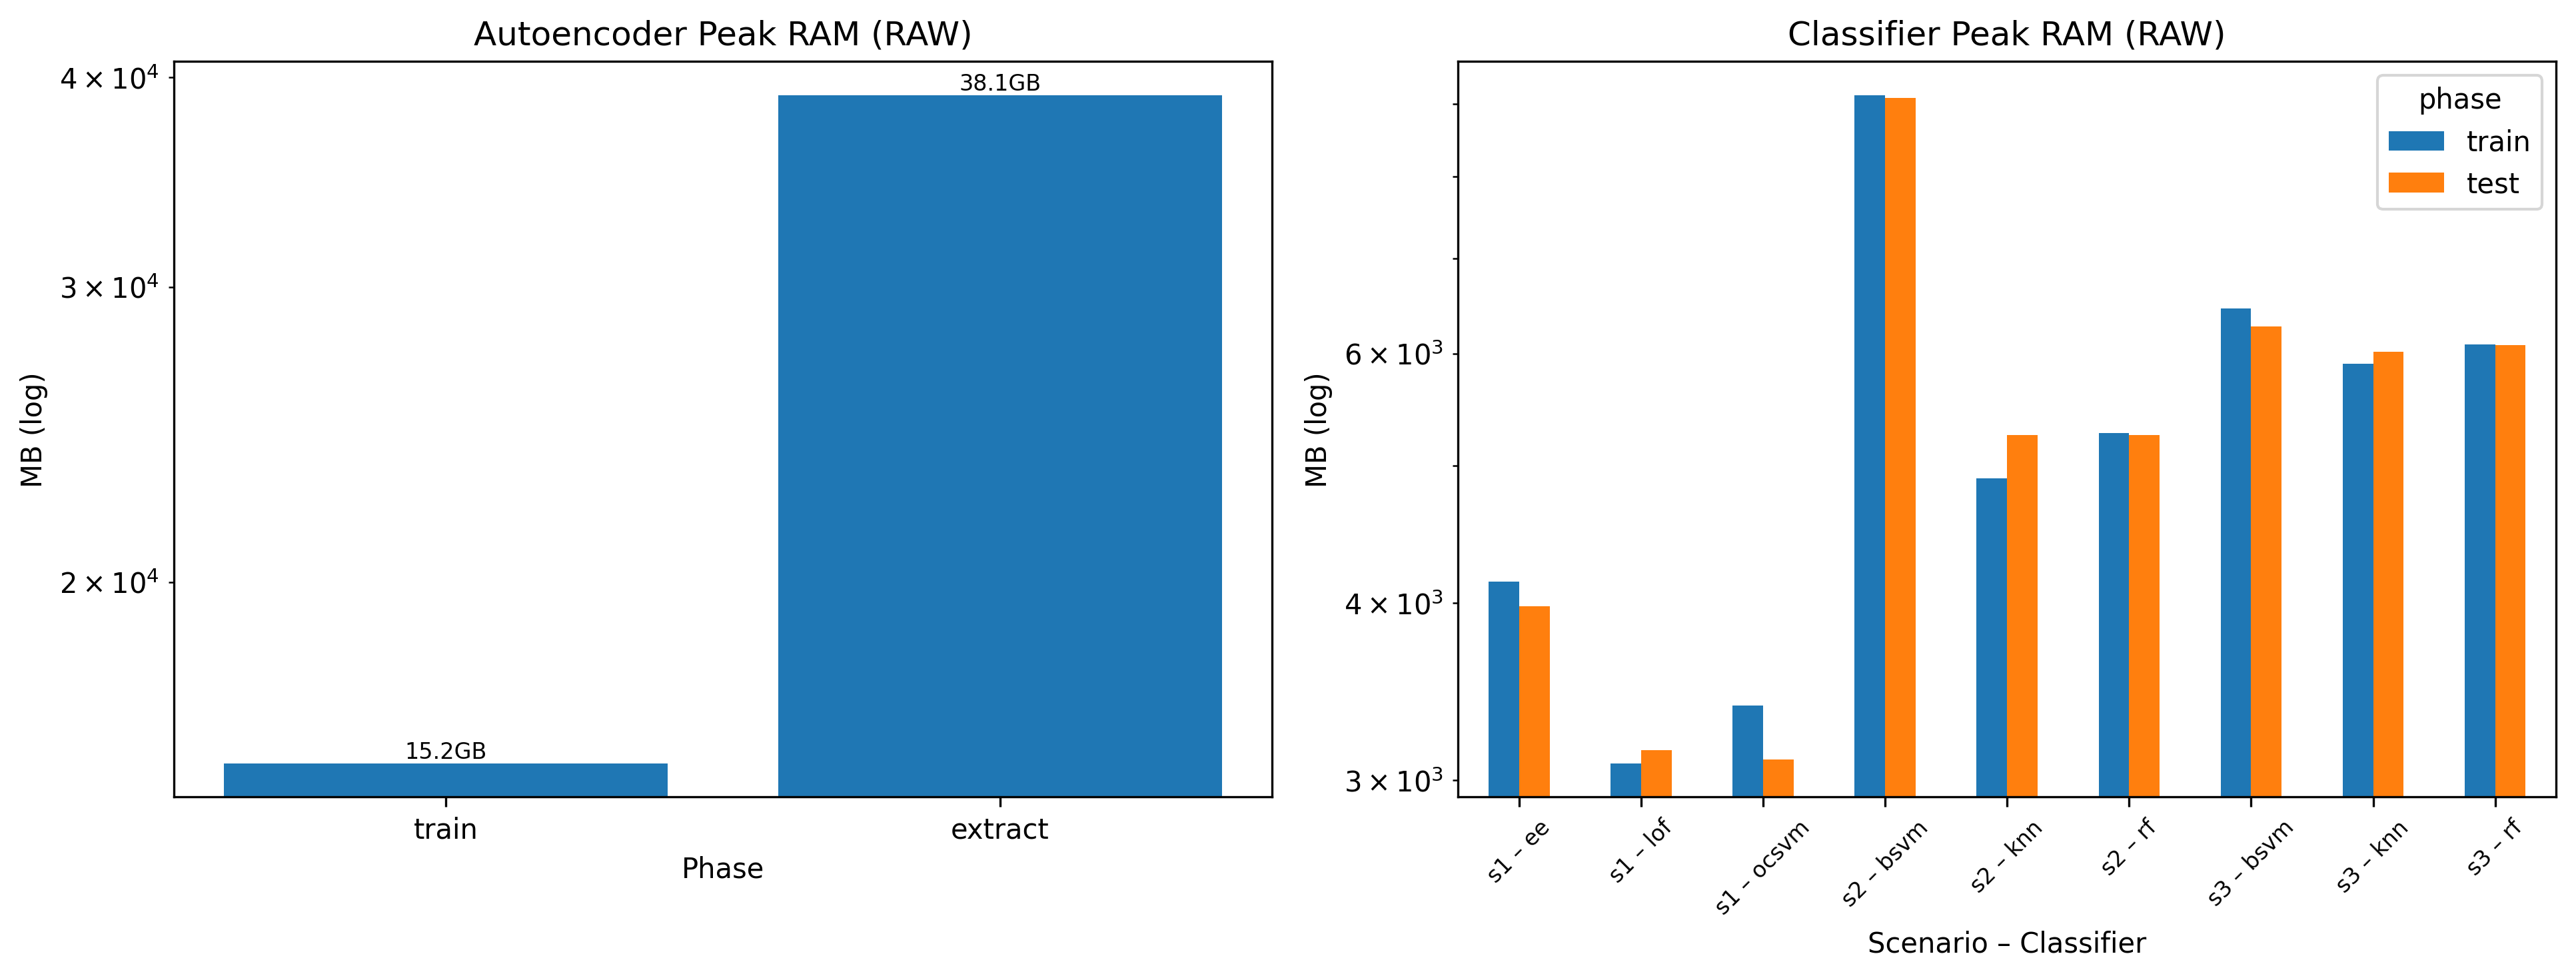
\includegraphics[width=\linewidth]{chapters/ram_raw.png}
	\caption{Memory Consumption — Feature Extraction and Traditional ML Models (RAW)}
	\label{fig:ram-raw}
\end{figure}

For the RAW representation (\cref{fig:ram-raw}), the feature extraction
stage dominates overall memory usage. While autoencoder training already
requires substantial memory, the encoding (feature extraction) phase
reaches the highest peak RAM values within the entire pipeline.
This indicates that processing and storing large byte-vector batches
constitutes the primary memory bottleneck.

In contrast, classifier memory usage remains moderate relative to
feature extraction. For RAW features, peak RAM consumption varies
considerably across scenarios. Scenario~1 exhibits comparatively low
memory usage, whereas Scenarios~2 and~3 require significantly more
memory. The highest peak occurs for Binary \ac{SVM} in Scenario~2,
reflecting the cost of handling high-dimensional feature spaces
with large training sets.

Across classifiers, training and testing phases show similar
memory profiles, indicating that model size and stored data
structures dominate memory requirements rather than temporary
computation during prediction.



\begin{figure}[!htbp]
	\centering
	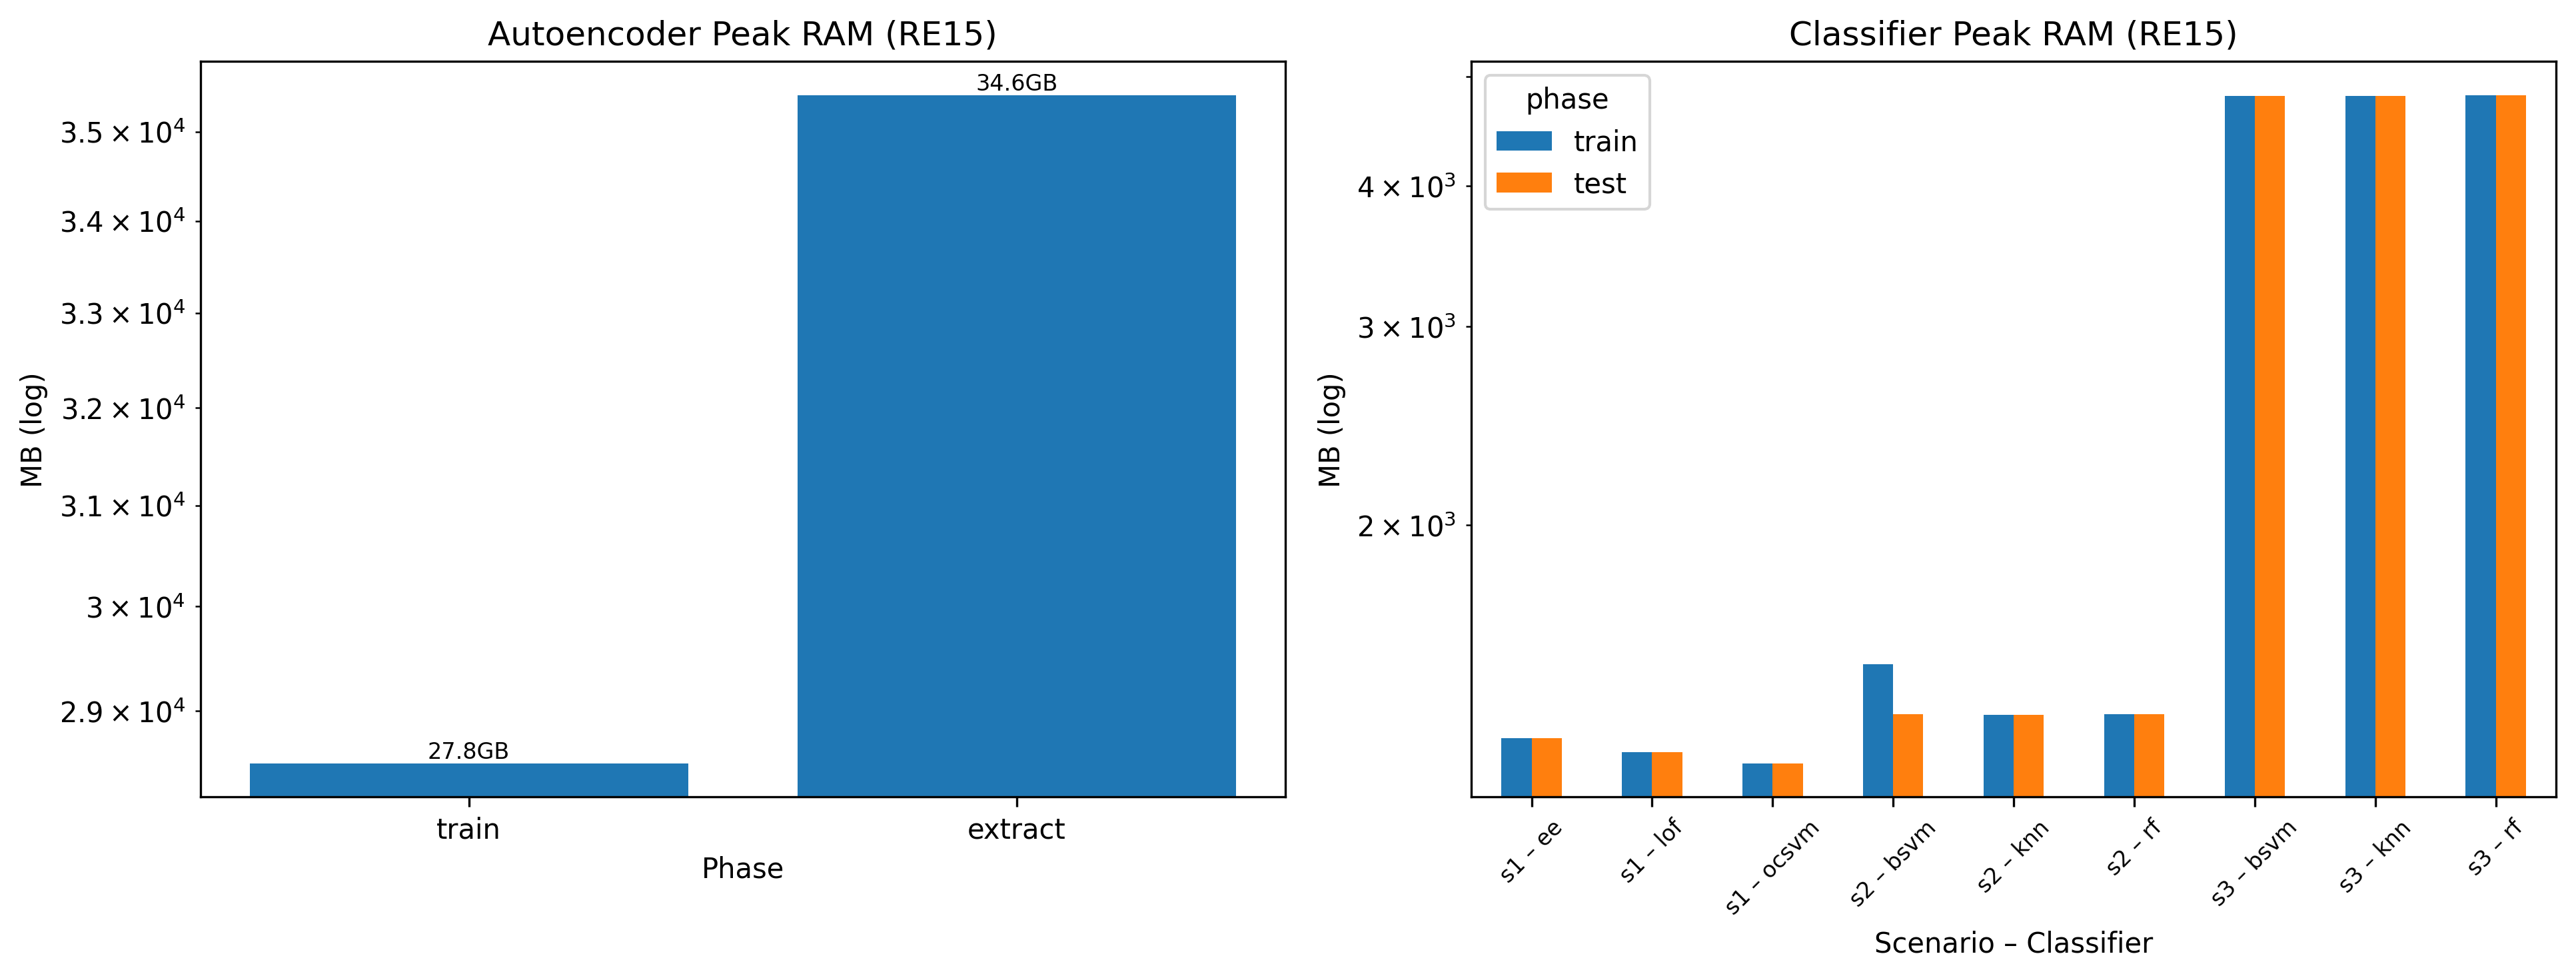
\includegraphics[width=\linewidth]{chapters/ram_re15.png}
	\caption{Memory Consumption — Feature Extraction and Traditional ML Models (RE15)}
	\label{fig:ram-re15}
\end{figure}

For the RE15 representation (\cref{fig:ram-re15}), overall memory
consumption is reduced compared to RAW, particularly at the
classifier stage. Nevertheless, the autoencoder remains the most
memory-intensive component. Interestingly, autoencoder training
requires more memory for RE15 than for RAW, suggesting that the
representation structure influences internal activation storage.

Classifier memory usage under RE15 is substantially lower in
Scenarios~1 and~2, but increases noticeably in Scenario~3.
This scenario-dependent behavior indicates that dataset composition
(e.g., class distribution and sample count) has a strong influence
on memory allocation.

Overall, RAW exhibits lower memory in Scenario~1 but significantly
higher memory in Scenarios~2 and~3, whereas RE15 maintains low
memory usage in the first two scenarios but shows a marked increase
in Scenario~3.


\section{\ac{DL} Models}

\begin{figure}[htb]
	\centering
	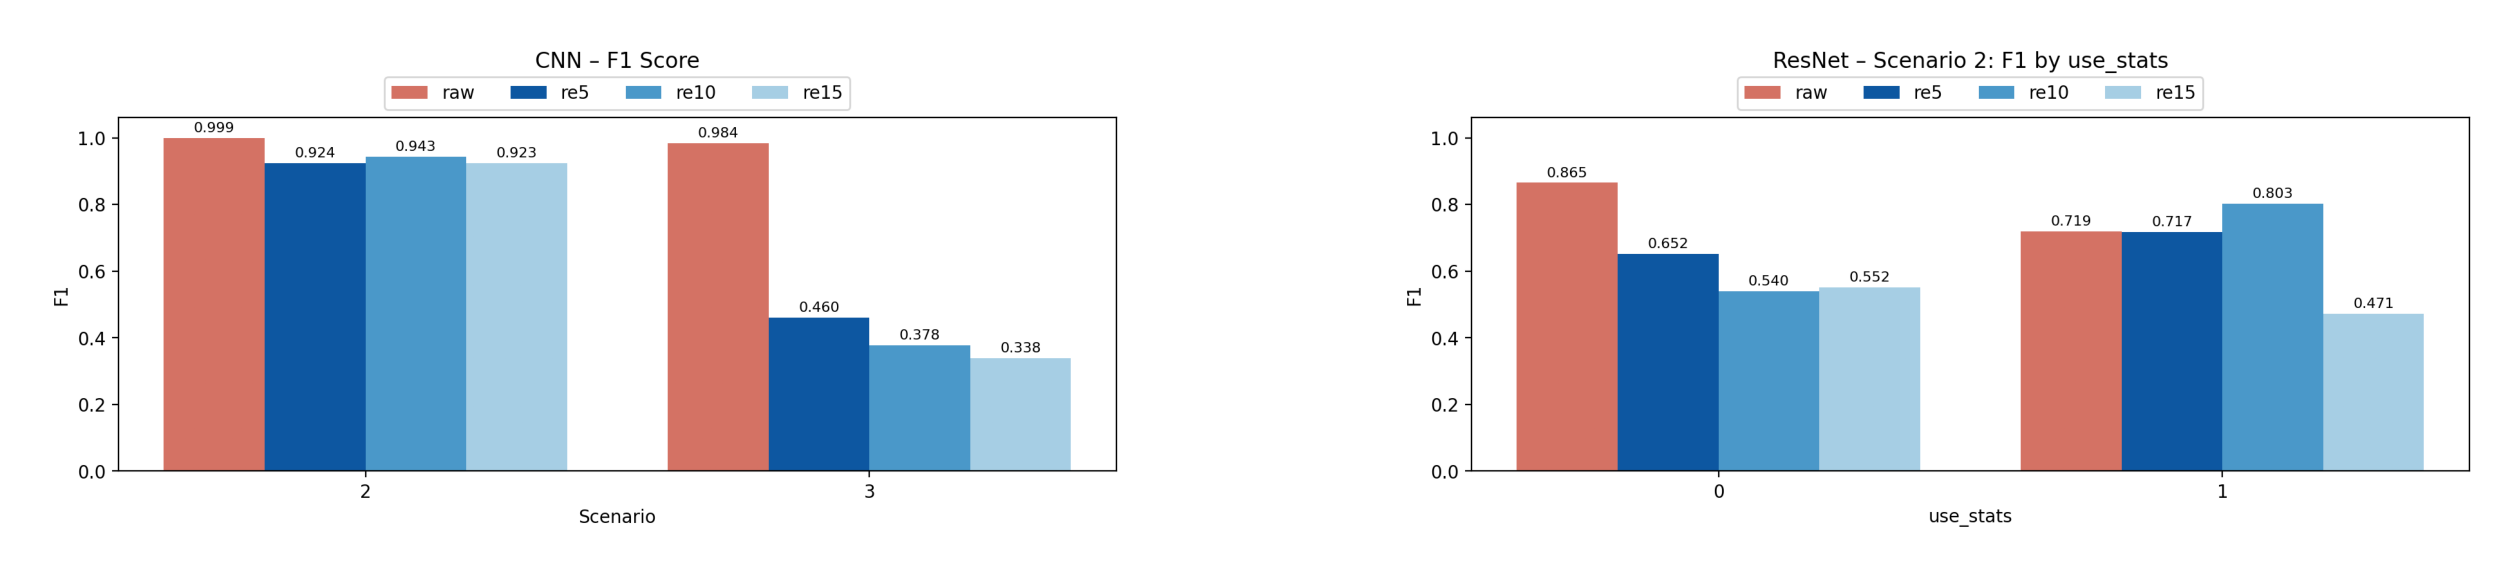
\includegraphics[width=\linewidth]{chapters/cnn_and_resnet_side_by_side.png}
	\caption{F1-scores of the CNN and ResNet classifiers across dataset representations}
	\label{fig:cnn-resnet}
\end{figure}

\subsection{\ac{CNN} Results}

The left panel of \cref{fig:cnn-resnet} summarizes the F1-scores of the
\ac{CNN} classifier for Scenarios~2 and~3 across the four dataset
representations (RAW, RE5, RE10, RE15). All \ac{CNN} models were trained
with oversampling to mitigate class imbalance effects.

Across all dataset types, Scenario~2 achieves consistently strong
performance. F1-scores exceed 0.9 for every representation,
with near-perfect detection for the RAW dataset. This indicates
that when sufficient labeled data and attack diversity are available,
the CNN can effectively learn discriminative byte-level patterns.

Although the reverse-engineered representations perform slightly
worse than RAW in Scenario~2, the differences among RE5, RE10,
and RE15 remain relatively small. Among them, RE10 achieves the
highest F1-score, suggesting that this representation offers a
balanced trade-off between compression and preserved structure.
Overall, the \ac{CNN} appears capable of partially compensating for
information loss in reduced representations when attack diversity
is sufficient.

In contrast, Scenario~3 shows a substantial performance drop for
all reverse-engineered datasets. Despite oversampling, F1-scores
decrease markedly, indicating limited generalization capability.
A likely explanation is the restricted diversity of attack types
in this scenario. While oversampling increases the number of
training instances, it does not introduce additional structural
variation, which limits the model’s ability to learn robust
decision boundaries.

Notably, the RAW representation maintains strong performance even
in Scenario~3. This suggests that full packet information provides
rich structural cues that remain discriminative even under
constrained attack configurations. In comparison, the
reverse-engineered representations appear to be limited more by
representational expressiveness than by class imbalance alone.

\subsection{ResNet}
The results obtained with the ResNet classifier in Scenario 2 show a clear impact of both reverse engineering and the inclusion of statistical features. When using raw packets without reverse engineering, the model achieved an F1-score of 0.865 without statistical features and 0.719 when statistical features were included. This indicates that raw packet information alone already provides strong discriminative signals for the classifier.

After applying reverse engineering, where only sequences of physical readings were used, the performance decreased. For p = 5, the F1-score dropped to 0.652, and further decreased to 0.540 for p = 10. A slight improvement was observed for p = 15, reaching 0.552, but the performance remained significantly below the raw packet baseline.

When statistical features were added to the ResNet input, their impact depended on the sequence length. For p = 5, the performance slightly improved to 0.717, suggesting that the additional statistical context helped compensate for the loss of structural packet information. For p = 10, the F1-score further increased to 0.803, representing the best result among the reverse-engineered inputs. However, for p = 15, the performance dropped significantly to 0.471, indicating that larger physical-reading sequences combined with statistical features may introduce noise or redundant information that negatively affects classification performance.

Overall, these results show that ResNet can effectively learn patterns from raw packet bytes, while its performance becomes more sensitive when only partial packet information is available.



\textbf{Comparison CNN ResNet}
A comparison between CNN and ResNet shows noticeable differences in their robustness across scenarios. For raw packets, both models achieved high performance, with CNN slightly outperforming ResNet, reaching an F1-score close to 0.999, while ResNet achieved 0.865. This indicates that CNN is particularly effective at learning local byte-level patterns in raw packet structures.

However, when reverse engineering was applied and only partial packet data was used, both models experienced a decline in performance. The CNN showed a sharper drop in Scenario 3, whereas the ResNet demonstrated more stable behavior when statistical features were included. In particular, ResNet benefited from the additional statistical features in some configurations, reaching 0.803 for p = 10, which suggests that the deeper architecture and residual connections may help integrate heterogeneous input features more effectively.

In summary, CNN achieves the best performance when complete packet structures are available, while ResNet shows slightly better adaptability when additional statistical features are incorporated into the model.

\section{Other Anomaly Detection Methods}
\begin{figure}[!htbp]
	\centering
	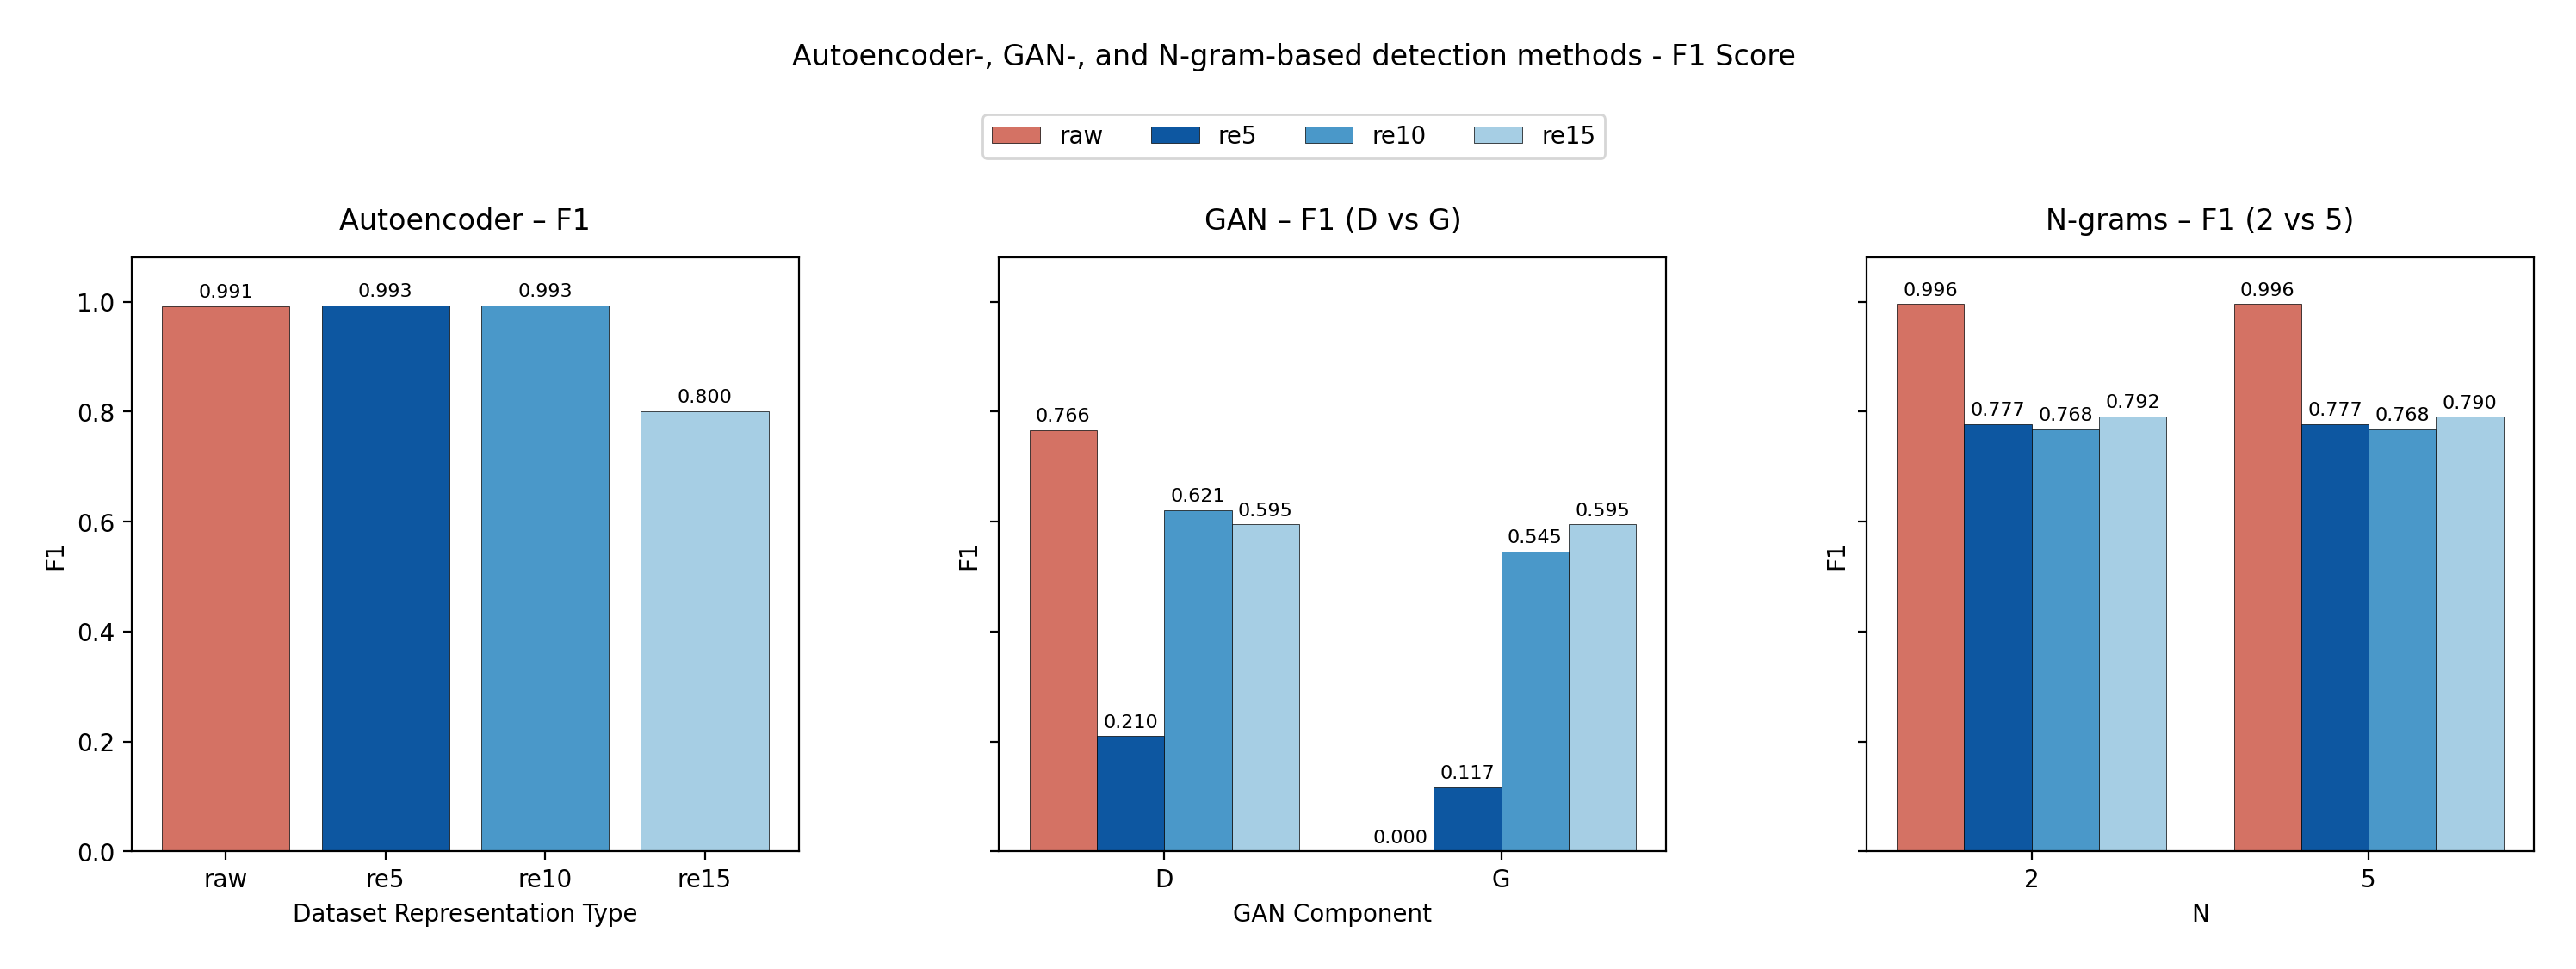
\includegraphics[width=\linewidth]{chapters/ae_gan_ngram_f1_combined.png}
	\caption{Autoencoder, GAN and N-Gram -based detection F1-Score}
     \label{fig:ae-gan-ngram}
\end{figure}


\textbf{Autoencoder}

The left panel of \cref{fig:ae-gan-ngram} summarizes the F1-scores of
the reconstruction-error-based \ac{SDA} classifier across the
different dataset representations (RAW, RE5, RE10, RE15).

For RAW, RE5, and RE10, the autoencoder achieves near-perfect
classification performance, with F1-scores close to 1.0.
Both precision and recall remain consistently high in these settings,
indicating that the learned reconstruction threshold effectively
separates benign and malicious traffic. Compared to RAW, the RE5
and RE10 representations even show slightly higher precision and
F1-scores, suggesting that moderate reverse engineering does not
degrade the discriminative power of the reconstruction-based method.

In contrast, performance drops dramatically for RE15.
The F1-score decreases sharply, accompanied by both low recall
and low precision. The reduced recall indicates that many attack
instances are incorrectly classified as benign (false negatives),
while the low precision reflects a substantial proportion of
false positives among predicted attacks. This behavior suggests
that the RE15 representation no longer preserves sufficient
structure for reliable reconstruction-based anomaly detection.

Overall, the results demonstrate that the \ac{SDA}-based
approach is highly effective for RAW and moderately reduced
representations (RE5, RE10), but becomes unstable when the
reverse-engineered representation is further compressed.

\textbf{GAN}

As shown in the middle panel of figure~\ref{fig:ae-gan-ngram}, the performance of the GAN-based approach is highly unstable and significantly lower compared to the other evaluated methods. While the discriminator achieves better results than the generator-based detection, its performance remains inferior to that of the \ac{SDA} and the N-gram models.

In particular, generator-based anomaly detection struggles considerably, especially when applied to raw packet data. We attribute this behavior to the inherent difficulty of generating valid raw network packets from random noise. Raw packets follow strict structural and syntactic constraints, including precise byte-level patterns and protocol-specific rules. Even minor deviations from these constraints can result in unrealistic or invalid packet representations.

Due to this high structural rigidity, the generator faces substantial challenges in learning an accurate representation of the underlying packet distribution. Consequently, the generated samples often fail to approximate realistic packet structures, leading to weaker anomaly detection performance.


\textbf{N-Gram}


The N-gram-based detection method demonstrates outstanding performance when applied to raw packet data, achieving an F1-score of approximately 0.996 as shown in the right panel of figure \ref{fig:ae-gan-ngram}. This near-perfect performance indicates that raw network packets contain highly distinctive local byte-sequence patterns that can be effectively captured by N-gram representations. Since raw packets include both protocol headers and payload information, they preserve structural regularities and fixed byte-level dependencies that strongly differentiate normal and malicious traffic.

After applying reverse engineering and restricting the input to physical readings only, a noticeable decrease in performance can be observed. Although the F1-score drops compared to the raw packet scenario, it remains relatively stable across different values of the concatenation parameter 
$p$. This stability suggests that increasing the number of concatenated physical readings does not significantly enhance or degrade the discriminating capability of the N-gram model.

The comparison between 2-gram and 5-gram configurations shows only marginal differences in performance. This indicates that extending the N-gram length does not substantially improve detection accuracy. In practice, shorter byte dependencies already capture most of the relevant structural information present in the packets. Larger N-grams may increase representational complexity, but they do not provide a significant additional benefit in this context.

The overall performance reduction observed after reverse engineering can be explained by the removal of protocol-related bytes. Raw packets contain strict and repetitive structural patterns defined by the underlying communication protocol. These regular patterns are highly suitable for modeling with N-grams, as they rely on local sequential dependencies. In contrast, physical readings are more variable and less structured at the byte level. As a result, the statistical regularities that N-grams exploit become weaker, leading to a reduced but still stable detection performance.


\textbf{Comparison AE, GAN, N-Gram}

Overall, the experimental results indicate that \ac{SDA}-based approaches provide the most robust and consistent performance across all evaluated scenarios. In particular, the stacked denoising autoencoder (SDA) maintains stable detection accuracy not only on raw packet data but also after reverse engineering and data reduction. This robustness suggests that representation-learning methods are well-suited for modeling both protocol-level structures and higher-level behavioral patterns in ICS traffic, even when structural information is partially removed.

The N-gram-based approach also demonstrates strong performance, especially when applied to raw packet data. Its effectiveness can be attributed to its ability to capture local byte-level patterns and repetitive protocol structures. However, its performance degrades once the input is restricted to physical readings only, indicating that it relies heavily on the structural regularities present in complete packet data. While N-grams remain competitive, their dependence on raw packet structure limits their generalizability in scenarios where protocol information is unavailable or intentionally removed.

In contrast, GAN-based methods exhibit unstable and comparatively weak performance. Although the discriminator performs moderately better than the generator-based detection, the overall results suggest that GANs are not well-suited for reliable anomaly detection at the byte level in ICS environments. The strict structural constraints and deterministic nature of raw network packets make it difficult for the generator to learn a realistic data distribution from noise. Consequently, the generated samples often fail to approximate valid packet structures, which negatively impacts detection performance.

In summary, representation-learning approaches such as autoencoders appear to be the most reliable choice for anomaly detection in proprietary ICS traffic. N-grams offer strong performance when full structural information is available, whereas GAN-based models struggle to provide stable and trustworthy results in this highly structured and safety-critical domain.

\section{Summary}


This section summarizes the main observations across all evaluated
approaches.

\subsection{Overall Model Performance}

Across all experiments, the strongest overall performance is achieved
by the reconstruction-based \ac{SDA}, the N-gram model,
and the \ac{CNN} classifier in Scenario~2.
In this setting, F1-scores approach near-perfect classification,
particularly for the RAW representation.

In contrast, GAN-based detection and traditional machine learning
classifiers exhibit the weakest overall performance.
While GAN models show moderate success in some configurations,
their results remain substantially below those of autoencoder- and
CNN-based approaches.
Traditional \ac{ML} classifiers are especially sensitive to the chosen
representation and scenario and frequently suffer from significant
performance degradation.

\subsection{Influence of Dataset Representation}

The RAW packet representation consistently yields the best results
across nearly all model families.
It preserves the full structural and contextual information of
network traffic, enabling both deep learning and classical models
to extract highly discriminative patterns.

The reverse-engineered representations (RE5, RE10, RE15) introduce
progressive aggregation and information reduction.
Among them, RE15—representing the strongest compression—produces
the weakest overall performance.
This indicates that aggressive abstraction of packet structure
removes discriminative signals that are essential for reliable
attack detection.

\subsection{Impact of Reverse Engineering Across Model Families}

The influence of reverse engineering differs substantially
between model classes.

Deep learning architectures such as \ac{CNN}, \ac{SDA},
and ResNet show comparatively robust behavior.
Although minor performance reductions occur for reduced
representations, these models remain competitive,
particularly when sufficient labeled data is available.
This suggests that deep architectures can internally learn
hierarchical feature representations that partially compensate
for information loss.

GAN-based and N-gram models exhibit moderate performance
degradation under reverse-engineered representations.
While still functional, their discriminative capacity decreases
more noticeably than for \ac{CNN} or \ac{SDA}.

The strongest negative impact is observed for traditional
machine learning classifiers.
These approaches rely explicitly on the extracted latent feature
vectors and do not perform hierarchical representation learning.
Consequently, they are more sensitive to the loss of structural
information introduced by reverse engineering.

\subsection{Impact of Evaluation Scenario}

Scenario characteristics have a strong influence on performance
across all models.
Scenario~2 consistently achieves the highest F1-scores,
indicating that models perform best when attack types are well
represented during training.

Scenario~3 yields the lowest overall performance.
The presence of unseen or highly constrained attack types
significantly reduces generalization capability, even for
strong deep learning models.
This highlights that attack diversity during training plays a
more decisive role than class imbalance alone.



       \chapter{Conclusion}
\label{chap:conclusion}



\section{Conclusion}

This study project investigated whether anomaly detection can operate
without explicit protocol knowledge while maintaining strong
performance on reverse-engineered traffic representations.

The results show that protocol-agnostic detection is feasible,
particularly when operating on raw packet data.
Autoencoder-based detection, CNN models, and N-gram approaches
achieve consistently strong performance, especially in
Scenario~2 where sufficient attack diversity is available.

Reverse engineering reduces computational cost but introduces
representation-dependent performance trade-offs.
While deep learning models remain comparatively robust under
moderate compression, traditional machine learning classifiers
experience significant degradation.
The most aggressively compressed representation (RE15) yields
the weakest overall results, indicating that critical structural
information is lost.

Scenario characteristics further influence performance:
limited attack diversity (Scenario~3) in the training data consistently reduces
generalization capability across all model families.

In summary, raw packet representations provide the most reliable
detection performance, whereas reverse-engineered representations
offer efficiency gains at the cost of reduced robustness.
The optimal choice therefore depends on the trade-off between
computational constraints and detection accuracy.

\section{Limitations}

Several limitations should be considered when interpreting the
results of this study project.

First, a post-hoc analysis revealed structural characteristics of
the dataset that may have influenced detection performance.
In particular, the attacker IP address appears to remain constant
across attack samples. Since the RAW representation includes full
packet headers, including IP-level information, models trained on
RAW data may have partially exploited this invariant identifier.
In contrast, the reverse-engineered representations exclude such
header information, which may contribute to the observed performance
gap between RAW and RE-based datasets. Consequently, the absolute
performance of RAW-based models should be interpreted with caution.

Second, attack labels were derived from the dataset folder structure
rather than from packet-level ground-truth annotations. As a result,
benign server responses that occurred within attack sessions were
also assigned the attack label. This introduces label noise and may
have affected both training and evaluation, particularly for models
sensitive to fine-grained traffic structure.

{\color{gray} Third, the reverse-engineered representation was designed to extract
a dynamic region within S7Comm payloads that was assumed to contain
process-related information. However, since the dataset does not
provide explicit ground-truth annotations for physical sensor values,
it cannot be guaranteed that the extracted region consistently
corresponds to actual physical readings. The extracted sequences
should therefore be interpreted as reverse-engineered payload
segments rather than verified process measurements.}
{\color{red} todo: describe physical readings problem correctly }


Finally, the evaluation was conducted on a specific dataset and
predefined scenarios. The observed trends may vary under different
network environments, attacker diversity, or alternative
reverse-engineering strategies. Future work should incorporate
datasets with greater attacker variability, stricter packet-level
labeling, and validated process-value annotations to further
assess robustness.

\section{Future Work}

The results of this study project open several avenues for further investigation.

The reverse-engineered representations rely on byte-level concatenation
of extracted payload segments. Although aggregation controlled by the
parameter $p$ increases contextual information, it may obscure
fine-grained temporal and structural dependencies within individual
packets. Future work could explore sequence-aware modeling approaches
that preserve packet boundaries or explicitly encode temporal order
instead of relying solely on concatenation.

The traditional ML classifiers operate on latent features extracted
by the stacked denoising autoencoder. While this compact representation
proved effective in certain settings, alternative feature extraction
strategies may further improve performance. For example, statistical
traffic descriptors, protocol-agnostic sequence embeddings, or
transformer-based encoders could provide richer and more expressive
representations for classical machine learning models.

Moreover, the evaluation was conducted on a dataset with specific
structural characteristics, including limited attacker diversity and
coarse-grained labeling. Future studies should therefore consider
more heterogeneous datasets with diversified attacker behavior,
strict packet-level annotations, and validated process-value ground
truth. Such validation would allow for a more robust assessment of
generalization performance under realistic industrial conditions.
	% add more chapters here

	% --------------------------------------------------------------------------
	% appendix after two clear pages
	\cleardoublepage{}
     \chapter{Appendix}

\section{Implementation of the ResNet Classifier}

This appendix presents the implementation of the ResNet-based classifier used in our experiments. The full implementation is provided in Listing~\ref{lst:resnet_code}. The code is written in Python using the PyTorch framework and follows the architectural requirements described in the project specification. 

The implemented model is a one-dimensional variant of the ResNet-18 architecture designed to process sequences of raw network packet bytes. Since network packets can be represented as sequences of byte values, a 1D convolutional architecture is used instead of the traditional 2D convolutional layers used in image processing.

The implementation consists of several main components:

\begin{itemize}

\item \textbf{Residual Blocks.}  
The model uses the BasicBlock structure of ResNet-18. Each block contains two convolutional layers followed by batch normalization and ReLU activation. A skip connection adds the input of the block to its output, enabling residual learning and improving gradient flow during training.

\item \textbf{ResNet Backbone.}  
The network contains four stages, each composed of two residual blocks, resulting in a total of 18 layers. The architecture follows the standard ResNet-18 layout adapted to 1D data. After the convolutional stages, an adaptive average pooling layer reduces the feature representation to a fixed-size embedding.

\item \textbf{Fully Connected Classification Head.}  
The extracted embedding is passed through two fully connected layers with dropout regularization before producing the final classification logits.

\item \textbf{Statistical Features.}  
In addition to raw packet bytes, the model optionally incorporates five statistical features derived from the packet content. These include:
\begin{itemize}
\item total number of bytes in the packet,
\item frequency of the most common byte,
\item frequency of the second most common byte,
\item Shannon entropy of the byte distribution,
\item fraction of zero bytes in the packet.
\end{itemize}

The entropy feature captures the randomness of the byte distribution, while the fraction of zero bytes helps detect padding patterns often introduced during packet normalization.

\item \textbf{Training Procedure.}  
The model is trained using the Adam optimizer and the categorical cross-entropy loss function. Early stopping is applied based on validation loss to prevent overfitting.

\item \textbf{Hyperparameter Search.}  
A grid search is performed over several training parameters, including the number of epochs, batch size, learning rate, and dropout probability. The combination yielding the highest average F1-score across the cross-validation folds is selected.

\item \textbf{Evaluation.}  
The implementation supports k-fold cross-validation and computes precision, recall, and F1-score for each fold. The final performance metrics are obtained by averaging the results across all folds.

\end{itemize}

The complete implementation used to run the ResNet experiments is provided below.

\begin{lstlisting}[language=Python, caption={Implementation of the ResNet classifier used in the experiments}, label={lst:resnet_code}]


import csv
from pathlib import Path

import numpy as np
import torch
import torch.nn.functional as F
from torch.utils.data import DataLoader, TensorDataset

from file_helper_t3 import load_k_fold_results
from labels_helper import deduplicate_folds, encode_labels
from handling_re_bytes_integrated import get_keep_indices_from_fold0_ae


# ---------------------------
# ResNet1D model definition
# ---------------------------

import torch
import torch.nn as nn
import torch.nn.functional as F


# -----------------------------
# 1) BasicBlock (1D) for ResNet-18
# -----------------------------
class BasicBlock1D(nn.Module):

    
    expansion = 1

    def __init__(self, in_channels: int, out_channels: int, stride: int = 1):
      
        # initialize parent class
        super().__init__()

      
        self.conv1 = nn.Conv1d(
            in_channels, out_channels,
            kernel_size=3, stride=stride, padding=1, bias=False
        )

        self.bn1 = nn.BatchNorm1d(out_channels)

        self.conv2 = nn.Conv1d(
            out_channels, out_channels,
            kernel_size=3, stride=1, padding=1, bias=False
        )

        # second batch normalization layer
        self.bn2 = nn.BatchNorm1d(out_channels)

        self.downsample = None
        if stride != 1 or in_channels != out_channels:
           
            self.downsample = nn.Sequential(
                nn.Conv1d(in_channels, out_channels, kernel_size=1, stride=stride, bias=False),
                nn.BatchNorm1d(out_channels),
            )

    def forward(self, x):
       
        # stores the input for skip connection
        identity = x

        # First conv + BN + ReLU
        out = self.conv1(x)
        out = self.bn1(out)
        out = F.relu(out, inplace=True)

        out = self.conv2(out)
        out = self.bn2(out)

        if self.downsample is not None:
            identity = self.downsample(identity)

        out = out + identity
        out = F.relu(out, inplace=True)
        return out


# -----------------------------
# 2) ResNet-18 backbone (1D): 4 stages, each stage has 2 blocks
# -----------------------------
class ResNet18_1D(nn.Module):
    

    def __init__(
        self,
        in_channels: int = 1,
        num_classes: int = 2,
        hidden_dim: int = 256,
        dropout_p: float = 0.3,
        use_stats: bool = False, # whether to use the 5 stats features
        stats_dim: int = 5, # number of stats features (if used)
    ):
        super().__init__()
        self.use_stats = use_stats
        self.stats_dim = stats_dim

       
        
        self.stem_conv = nn.Conv1d(in_channels, 64, kernel_size=7, stride=2, padding=3, bias=False)
        self.stem_bn = nn.BatchNorm1d(64)
        self.stem_pool = nn.MaxPool1d(kernel_size=3, stride=2, padding=1)

       
       
        self.in_planes = 64
        # the 4 stages
        self.layer1 = self._make_layer(out_channels=64,  blocks=2, stride=1)
        self.layer2 = self._make_layer(out_channels=128, blocks=2, stride=2)
        self.layer3 = self._make_layer(out_channels=256, blocks=2, stride=2)
        self.layer4 = self._make_layer(out_channels=512, blocks=2, stride=2)

        # Pooling -> embedding
       
        self.avgpool = nn.AdaptiveAvgPool1d(1)

        # FC head (2 FC layers)
       
        fc1_in = embedding_dim + (stats_dim if use_stats else 0)

        self.fc1 = nn.Linear(fc1_in, hidden_dim)
        self.drop = nn.Dropout(p=dropout_p)
        self.fc2 = nn.Linear(hidden_dim, num_classes)

        # init like typical ResNet
        self._init_weights()

    def _make_layer(self, out_channels: int, blocks: int, stride: int):
        layers = []
        # First block may downsample via stride
        layers.append(BasicBlock1D(self.in_planes, out_channels, stride=stride))
        self.in_planes = out_channels * BasicBlock1D.expansion
        # Remaining blocks keep stride=1
        for _ in range(1, blocks):
            layers.append(BasicBlock1D(self.in_planes, out_channels, stride=1))
        return nn.Sequential(*layers)

    def _init_weights(self):
        
        for m in self.modules():
            if isinstance(m, nn.Conv1d):
                nn.init.kaiming_normal_(m.weight, mode="fan_out", nonlinearity="relu")
            elif isinstance(m, nn.BatchNorm1d):
                nn.init.ones_(m.weight)
                nn.init.zeros_(m.bias)

    def forward(self, x, stats=None):
       
        # Stem
        x = self.stem_conv(x)
        x = self.stem_bn(x)
        x = F.relu(x, inplace=True)
        x = self.stem_pool(x)

        # Stages
        x = self.layer1(x)
        x = self.layer2(x)
        x = self.layer3(x)
        x = self.layer4(x)

        # Adaptive pooling -> (B, 512, 1) -> flatten -> (B, 512)
        x = self.avgpool(x)
        x = torch.flatten(x, 1)

        # Optionally concatenate stats features
        if self.use_stats:
            if stats is None:
                raise ValueError("use_stats=True but stats=None was passed to forward().")
            if stats.dim() != 2 or stats.size(1) != self.stats_dim:
                raise ValueError(f"stats must be (B,{self.stats_dim}), got {tuple(stats.shape)}.")
            x = torch.cat([x, stats], dim=1)

        # FC head: FC1 + ReLU + Dropout, then FC2 -> logits
        x = self.fc1(x)
        x = F.relu(x, inplace=True)
        x = self.drop(x)
        logits = self.fc2(x)
        return logits




# -----------------------------
# Metrics (same as your CNN file)
# -----------------------------
def precision_recall_f1(y_true, y_pred):
    y_true = np.asarray(y_true)
    y_pred = np.asarray(y_pred)

    tp = np.sum((y_true == 1) & (y_pred == 1))
    fp = np.sum((y_true == 0) & (y_pred == 1))
    fn = np.sum((y_true == 1) & (y_pred == 0))

    precision = tp / (tp + fp) if (tp + fp) else 0.0
    recall    = tp / (tp + fn) if (tp + fn) else 0.0
    f1        = (2 * precision * recall / (precision + recall)) if (precision + recall) else 0.0
    return float(precision), float(recall), float(f1)


# -----------------------------
# 5 stats features (optional)
# Sheet requires first 3 + 2 proposed :contentReference[oaicite:1]{index=1}
# Proposed extras here:
#   - Shannon entropy of bytes (captures "randomness/structure")
#   - Fraction of zero bytes (captures padding / sparsity patterns)
# -----------------------------
def _shannon_entropy_from_counts(counts: np.ndarray) -> float:
    
    # total number of observed bytes in the histogram
    total = counts.sum()

    # handle edge case of no bytes
    if total <= 0:
        return 0.0

    # convert counts into probabilities of each byte value for non-zero bins only
    p = counts[counts > 0].astype(np.float64) / float(total)

    # compute Shannon entropy -p log2(p) summed over all byte values
    # 0 or 1 entropy if all bytes are the same, and 0.5 is complete uncertainty
    return float(-(p * np.log2(p)).sum())


def compute_stats_features(
    X_bytes: np.ndarray,
    pad_value: int = 0,
    padded: bool = True,
) -> np.ndarray:
   
    X = X_bytes
    if X.dtype != np.uint8:
        X = X.astype(np.uint8)

    N, M = X.shape
    feats = np.zeros((N, 5), dtype=np.float32)

    for i in range(N):
        row = X[i]

        # "total bytes before trimming/padding" requirement :contentReference[oaicite:2]{index=2}
        # If you only have padded arrays, best practical approximation:
        # count non-pad bytes when padding exists, else M.
        if padded:
            total_bytes = int(np.sum(row != pad_value))
            if total_bytes == 0:
                total_bytes = M
        else:
            total_bytes = M
        counts = np.bincount(row, minlength=256)

        # top-2 frequencies
        top2 = np.sort(counts)[-2:]
        top1_count = int(top2[-1])
        top2_count = int(top2[-2])

        ent = _shannon_entropy_from_counts(counts)

        # this tells the model how much of the fixed-length input is artificial. 
        frac_pad = float(counts[pad_value]) / float(M) if M > 0 else 0.0

        # store features
        feats[i, 0] = float(total_bytes)
        feats[i, 1] = float(top1_count)
        feats[i, 2] = float(top2_count)
        feats[i, 3] = float(ent)
        feats[i, 4] = float(frac_pad)

    return feats


# -----------------------------
# Data split for ResNet (PyTorch)
# -----------------------------
def split_training_and_test_resnet(ds, labels, train_indices_fold, test_indices_fold, M: int):
   
    X_train = ds[train_indices_fold]
    X_test  = ds[test_indices_fold]

    # ensure length M (truncate or pad)
    def _fix_len(X):
        if X.shape[1] == M:
            return X
        if X.shape[1] > M:
            return X[:, :M]
        # pad with 0
        pad = np.zeros((X.shape[0], M - X.shape[1]), dtype=X.dtype)
        return np.concatenate([X, pad], axis=1)

    X_train = _fix_len(X_train)
    X_test  = _fix_len(X_test)

    # keep raw bytes for stats (uint8)
    X_train_raw = X_train.astype(np.uint8, copy=False)
    X_test_raw  = X_test.astype(np.uint8, copy=False)

    # normalize to [0,1] and make (N,1,M) to be tensor
    X_train_t = (X_train.astype(np.float32) / 255.0)[:, None, :]
    X_test_t  = (X_test.astype(np.float32) / 255.0)[:, None, :]

    y_train = labels[train_indices_fold].astype(np.int64)
    y_test  = labels[test_indices_fold].astype(np.int64)

    return X_train_t, X_test_t, y_train, y_test, X_train_raw, X_test_raw


# -----------------------------
# Train/Eval ResNet
# -----------------------------
def train_resnet(
    model: torch.nn.Module,
    train_loader: DataLoader,
    val_loader: DataLoader,
    epochs: int = 15,
    lr: float = 1e-3,
    weight_decay: float = 0.0,
    patience: int = 3,
    device: str = "cuda",
):
    # using Adam optimizer
    opt = torch.optim.Adam(model.parameters(), lr=lr, weight_decay=weight_decay)

    # best values tracker
    best_val = float("inf")
    best_state = None

    # Counts how many consecutive epochs did not improve validation loss.
    bad = 0

    # epochs excution
    for _epoch in range(epochs):

        # training
        model.train()
        for batch in train_loader:
            # unpack batch depending on whether stats features exist
            if len(batch) == 2:
                xb, yb = batch
                sb = None # statistics features batch
            else:
                xb, sb, yb = batch

            # move to device
            xb = xb.to(device, non_blocking=True)
            yb = yb.to(device, non_blocking=True)
            if sb is not None:
                sb = sb.to(device, non_blocking=True)
            # forward + backward + optimize steps
            opt.zero_grad(set_to_none=True)
            logits = model(xb, stats=sb) if sb is not None else model(xb)
            loss = F.cross_entropy(logits, yb)
            loss.backward()
            opt.step()

        # validation
        model.eval()
        val_loss = 0.0
        n = 0
        with torch.no_grad():
            for batch in val_loader:
                # same unpacking logic
                if len(batch) == 2:
                    xb, yb = batch
                    sb = None
                else:
                    xb, sb, yb = batch
                xb = xb.to(device, non_blocking=True)
                yb = yb.to(device, non_blocking=True)
                if sb is not None:
                    sb = sb.to(device, non_blocking=True)

                # forward pass + loss computation
                logits = model(xb, stats=sb) if sb is not None else model(xb)
                loss = F.cross_entropy(logits, yb)
                bs = xb.size(0)
                val_loss += float(loss) * bs
                n += bs

        # average validation loss, and avoid division by zero
        val_loss = val_loss / max(n, 1)

        # early stopping check 
        if val_loss < best_val:
            best_val = val_loss
            best_state = {k: v.detach().cpu().clone() for k, v in model.state_dict().items()}
            bad = 0
        else:
            bad += 1
            if bad >= patience:
                break
    # restore best weights at the end from checkpoints. 
    if best_state is not None:
        model.load_state_dict(best_state)

# -----------------------------

def evaluate_resnet(
    model: torch.nn.Module,
    test_loader: DataLoader,
    device: str = "cuda",
):
    model.eval()
    y_true = []
    y_pred = []

    with torch.no_grad():
        for batch in test_loader:
            # same unpacking logic
            if len(batch) == 2:
                xb, yb = batch
                sb = None
            else:
                xb, sb, yb = batch

            xb = xb.to(device, non_blocking=True)
            if sb is not None:
                sb = sb.to(device, non_blocking=True)

            logits = model(xb, stats=sb) if sb is not None else model(xb)
            preds = torch.argmax(logits, dim=1).cpu().numpy()

            y_pred.append(preds)
            y_true.append(yb.numpy())
    # concatenate all batches
    y_true = np.concatenate(y_true)
    y_pred = np.concatenate(y_pred)

    # compute metrics
    p, r, f1 = precision_recall_f1(y_true, y_pred)
    return p, r, f1, y_pred


# -----------------------------
# One fold execution
# -----------------------------
def execute_fold_resnet(
    fold_idx: int,
    binary_numeric_labels: np.ndarray,
    scenario: int,
    param: int,
    train_idx,
    test_idx,
    M: int,
    use_stats: bool = False,
    stats_dim: int = 5,
    epochs: int = 15,
    batch_size: int = 256,
    lr: float = 1e-3,
    dropout_p: float = 0.3,
    hidden_dim: int = 256,
    weight_decay: float = 0.0,
    device: str | None = None,
    debug_subset: bool = True,  # mimic your CNN "first+last 1000"
):
    if device is None:
        device = "cuda" if torch.cuda.is_available() else "cpu"

    # ---- load dataset ----
    if param != 0:
        ds = np.load(f"datasets/re_bytes_{param}.npy")
        print(f"Experiment: ResNet classifier, fold {fold_idx}, scenario {scenario}, RE{param}, stats={use_stats}")
    else:
        ds = np.load("datasets/raw_bytes.npy")
        print(f"Experiment: ResNet classifier, fold {fold_idx}, scenario {scenario}, RAW, stats={use_stats}")

    # split -> normalize -> (N,1,M)
    X_train, X_test, y_train, y_test, X_train_raw, X_test_raw = split_training_and_test_resnet(
        ds, binary_numeric_labels, np.array(train_idx), np.array(test_idx), M=M
    )

    # optional small subset (same spirit as your CNN demo)
    if debug_subset and len(X_train) > 2000:
        first = np.arange(0, 1000)
        last  = np.arange(len(X_train) - 1000, len(X_train))
        sel = np.concatenate([first, last])
        X_train = X_train[sel]
        y_train = y_train[sel]
        X_train_raw = X_train_raw[sel]

    # stats (if enabled)
    if use_stats:
        S_train = compute_stats_features(X_train_raw)  # (Ntr,5)
        S_test  = compute_stats_features(X_test_raw)   # (Nte,5)
        S_train_t = torch.from_numpy(S_train)
        S_test_t  = torch.from_numpy(S_test)
    else:
        S_train_t = None
        S_test_t  = None

    # tensors
    X_train_t = torch.from_numpy(X_train)
    y_train_t = torch.from_numpy(y_train)
    X_test_t  = torch.from_numpy(X_test)
    y_test_t  = torch.from_numpy(y_test)

    # train/val split
    n = len(X_train_t)
    perm = torch.randperm(n)
    val_n = max(1, int(0.1 * n))
    val_idx = perm[:val_n]
    tr_idx  = perm[val_n:]

    if use_stats:
        train_ds = TensorDataset(X_train_t[tr_idx], S_train_t[tr_idx], y_train_t[tr_idx])
        val_ds   = TensorDataset(X_train_t[val_idx], S_train_t[val_idx], y_train_t[val_idx])
        test_ds  = TensorDataset(X_test_t, S_test_t, y_test_t)
    else:
        train_ds = TensorDataset(X_train_t[tr_idx], y_train_t[tr_idx])
        val_ds   = TensorDataset(X_train_t[val_idx], y_train_t[val_idx])
        test_ds  = TensorDataset(X_test_t, y_test_t)

    train_loader = DataLoader(train_ds, batch_size=batch_size, shuffle=True, drop_last=False)
    val_loader   = DataLoader(val_ds, batch_size=batch_size, shuffle=False, drop_last=False)
    test_loader  = DataLoader(test_ds, batch_size=batch_size, shuffle=False, drop_last=False)

    # model
    model = ResNet18_1D(
        in_channels=1,
        num_classes=2,
        hidden_dim=hidden_dim,
        dropout_p=dropout_p,
        use_stats=use_stats,
        stats_dim=stats_dim,
    ).to(device)

    train_resnet(
        model=model,
        train_loader=train_loader,
        val_loader=val_loader,
        epochs=epochs,
        lr=lr,
        weight_decay=weight_decay,
        patience=3,
        device=device,
    )

    # eval
    p, r, f1, _ = evaluate_resnet(model=model, test_loader=test_loader, device=device)
    return p, r, f1


# -----------------------------
# Run ResNet for a scenario + representation
# -----------------------------
def run_resnet_for_scenario(
    scenario: int,
    prefix_for_files: str,   # "raw" or "re"
    global_label_encoder,
    keep_indices,
    param: int,
    M: int,
    use_stats: bool = False,
    stats_dim: int = 5,
    epochs: int = 15,
    batch_size: int = 256,
    lr: float = 1e-3,
    dropout_p: float = 0.3,
    hidden_dim: int = 256,
    weight_decay: float = 0.0,
):
    labels = np.load(f"datasets/{prefix_for_files}_labels.npy")

    train_indices, test_indices = load_k_fold_results(
        f"k_fold_results/k_fold_s{scenario}_{prefix_for_files}.json"
    )

    if param != 0:
        train_indices, test_indices = deduplicate_folds(train_indices, test_indices, keep_indices)

    numeric_labels = encode_labels(global_label_encoder, labels)
    binary_numeric_labels = np.where(numeric_labels == 0, 0, 1)

    k = len(train_indices)

    # Fine-tuning hyperparameters
    epochss = [15, 20, 25,30]
    batch_sizes = [256, 512, 1024]
    lrs = [1e-3, 5e-4, 1e-4]
    dropout_ps = [0.3, 0.5, 0.7]
    
    best_epoch = -1
    best_bs = -1
    best_lr = -1
    best_dps = -1 

    best_f1 = 0
    best_percision = 0
    best_recall = 0

    for e in epochss:
        for bs in batch_sizes:
            for learning_rate in lrs:
                for dp in dropout_ps:          
                    print(f'running with current parameters: epochs={e}, batch_size={bs}, learning_rate={learning_rate}, dropout_p={dp}')        
                    precisions, recalls, f1s = [], [], []
                    for fold_idx in range(k):
                        if len(train_indices[fold_idx]) == 0 or len(test_indices[fold_idx]) == 0:
                            continue

                        p, r, f1 = execute_fold_resnet(
                            fold_idx=fold_idx,
                            binary_numeric_labels=binary_numeric_labels,
                            scenario=scenario,
                            param=param,
                            train_idx=train_indices[fold_idx],
                            test_idx=test_indices[fold_idx],
                            M=M,
                            use_stats=use_stats,
                            stats_dim=stats_dim,
                            epochs=e,
                            batch_size=bs,
                            lr=learning_rate,
                            dropout_p=dp,
                            hidden_dim=hidden_dim,
                            weight_decay=weight_decay,
                        )

                        precisions.append(p)
                        recalls.append(r)
                        f1s.append(f1)
                        print(f"[Fold {fold_idx}] P={p:.4f} R={r:.4f} F1={f1:.4f}")
                    avg_f1 = float(np.mean(f1s))
                    if avg_f1 > best_f1:
                        best_f1 = avg_f1
                        best_percision = float(np.mean(precisions))
                        best_recall = float(np.mean(recalls))
                        best_epoch = e
                        best_bs = bs
                        best_lr = learning_rate
                        best_dps = dp
    # if len(precisions) == 0:
    #     return 0.0, 0.0, 0.0
    print(f'best parameters are: {best_epoch}, {best_bs}, {best_lr}, {best_dps}')
    print(f'best results: P={best_percision:.4f} R={best_recall:.4f} F1={best_f1:.4f}')

    return best_percision, best_recall, best_f1  
    return float(np.mean(precisions)), float(np.mean(recalls)), float(np.mean(f1s))


def run_resnet_classifier_on_dataset(
    scenario: int,
    prefix: str,               # "raw", "re5", "re10", "re15" (only used for naming)
    param: int,                # 0, 5, 10, 15
    global_label_encoder,
    M: int,
    use_stats: bool = False,
    out_csv: str = "results/resnet_summary.csv",
):
    if param != 0:
        keep_indices = get_keep_indices_from_fold0_ae(f"datasets/re_bytes_{param}.npy")
        prefix_for_files = "re"
    else:
        keep_indices = []
        prefix_for_files = "raw"

    avg_p, avg_r, avg_f1 = run_resnet_for_scenario(
        scenario=scenario,
        prefix_for_files=prefix_for_files,
        global_label_encoder=global_label_encoder,
        keep_indices=keep_indices,
        param=param,
        M=M,
        use_stats=use_stats,
        stats_dim=5,
    )

    out_dir = Path("results")
    out_dir.mkdir(exist_ok=True)

    summary_path = Path(out_csv)
    write_header = not summary_path.exists()

    representation = "raw" if param == 0 else f"re{param}"

    with summary_path.open("a", newline="") as f:
        w = csv.writer(f)
        if write_header:
            w.writerow(["scenario", "representation", "M", "use_stats", "avg_precision", "avg_recall", "avg_f1"])
        w.writerow([scenario, representation, M, int(use_stats), f"{avg_p:.6f}", f"{avg_r:.6f}", f"{avg_f1:.6f}"])

    return avg_p, avg_r, avg_f1


# -----------------------------
# The function you asked for:
# similar to run_experiment_cnn_classifier
# -----------------------------
def run_experiment_resnet_classifier(global_label_encoder, M_raw, M_re):
   
    prefixes = ["raw", "re5", "re10", "re15"]
    params = [0, 5, 10, 15]

    results = {}
    for scenario in (2, 3):
        results[scenario] = {}
        for prefix, param in zip(prefixes, params):
            M = M_raw if param == 0 else M_re

            # no-stats
            key0 = f"{prefix}_nostats"
            results[scenario][key0] = run_resnet_classifier_on_dataset(
                scenario=scenario,
                prefix=prefix,
                param=param,
                global_label_encoder=global_label_encoder,
                M=M,
                use_stats=False,
                out_csv="results/resnet_summary.csv",
            )

            # with-stats
            key1 = f"{prefix}_withstats"
            results[scenario][key1] = run_resnet_classifier_on_dataset(
                scenario=scenario,
                prefix=prefix,
                param=param,
                global_label_encoder=global_label_encoder,
                M=M,
                use_stats=True,
                out_csv="results/resnet_summary.csv",
            )

    return results

\end{lstlisting}


\section{Implementation of the GAN-based Anomaly Detector}

This appendix presents the implementation of the Generative Adversarial Network (GAN) used for anomaly detection in industrial control system (ICS) network traffic. The full implementation is provided in Listing~\ref{lst:gan_code}. The code is implemented in Python using the PyTorch deep learning framework.

The implemented GAN consists of two main components: a \textit{generator} and a \textit{discriminator}. The generator learns to produce synthetic packet representations, while the discriminator attempts to distinguish between real network packets and generated samples. Through this adversarial training process, the discriminator learns meaningful representations of normal network traffic, which can later be used for anomaly detection.

\subsection{Discriminator Architecture}

The discriminator is implemented as a modular model composed of two parts: a feature extractor and a classifier. This design allows the model to expose intermediate feature representations that are later used for feature matching during GAN training.

\begin{itemize}

\item \textbf{Feature Extractor.}  
The feature extractor consists of nine convolutional layers using two-dimensional convolutions. The input data is represented as a tensor of shape $(batch\_size, 1, m, n)$, where $m$ denotes the number of packets in a sequence and $n$ denotes the number of bytes per packet. 

Each convolutional layer is followed by a ReLU activation function. Dropout regularization is applied after most convolutional layers in order to improve generalization and reduce overfitting. The number of filters gradually increases across layers, enabling the network to learn hierarchical representations of packet structures. After the convolutional layers, an adaptive average pooling layer reduces the spatial dimensions and produces a compact feature representation.

\item \textbf{Classifier.}  
The extracted feature vector is passed to a fully connected classifier composed of four dense layers with ReLU activation functions. The final layer outputs a single value representing the discriminator score, which indicates how likely the input sample is to belong to the real data distribution.

\item \textbf{Wrapper Model.}  
The final discriminator model combines the feature extractor and the classifier into a single module. This wrapper enables two types of forward passes:
\begin{itemize}
\item extraction of intermediate feature representations used for feature matching loss,
\item computation of the final real/fake score used during adversarial training.
\end{itemize}

\end{itemize}

\subsection{Generator Architecture}

The generator network is designed to transform random noise vectors into synthetic packet representations that resemble real ICS network traffic.

The generator receives a noise vector $z \sim \mathcal{N}(0,1)$ with dimensionality $m \times n$. The architecture consists of two main stages:

\begin{itemize}

\item \textbf{Fully Connected Layers.}  
The first stage contains four fully connected layers with LeakyReLU activation functions. These layers expand the noise vector into a high-dimensional representation suitable for convolutional processing.

\item \textbf{Convolutional Layers.}  
The second stage consists of eight convolutional layers that progressively transform the intermediate representation into a tensor with the same spatial dimensions as the input packet representation $(1, m, n)$. The first four convolutional layers are preceded by upsampling operations, enabling the generator to construct spatial structure in the generated packets.

The final convolutional layer uses a sigmoid activation function to ensure that the generated values lie within the normalized range of the packet data.

\end{itemize}

\subsection{Model Integration}

During training, the generator and discriminator are optimized in an adversarial manner. The discriminator learns to differentiate between real network packets and generated samples, while the generator attempts to produce samples that the discriminator cannot distinguish from real data. In addition to the standard adversarial objective, the discriminator features are used for feature matching in order to stabilize training.

The complete implementation of the GAN components used in our experiments is shown below.

\begin{lstlisting}[language=Python, caption={Implementation of the GAN discriminator and generator models}, label={lst:gan_code}]

import torch
import torch.nn as nn


class Generator(nn.Module):
    def __init__(self, m, n, kernel_size=3):
        super().__init__()

        self.m = m
        self.n = n
        self.z_dim = m * n

        # -------- Stage 1: Fully Connected layers --------
        self.fc = nn.Sequential(
            nn.Linear(self.z_dim, 512),
            nn.LeakyReLU(0.2),

            nn.Linear(512, 1024),
            nn.LeakyReLU(0.2),

            nn.Linear(1024, 2048),
            nn.LeakyReLU(0.2),

            nn.Linear(2048, 256 * m * n),
            nn.LeakyReLU(0.2)
        )

        # -------- Stage 2 & 3: Convolutional layers --------
        self.conv_layers = nn.Sequential(
            # Upsampling + Conv (1)
            nn.Upsample(scale_factor=1),  # placeholder (keeps shape explicit)
            nn.Conv2d(256, 256, kernel_size=kernel_size, padding=1),
            nn.LeakyReLU(0.2),

            # Upsampling + Conv (2)
            nn.Upsample(scale_factor=1),
            nn.Conv2d(256, 256, kernel_size=kernel_size, padding=1),
            nn.LeakyReLU(0.2),

            # Upsampling + Conv (3)
            nn.Upsample(scale_factor=1),
            nn.Conv2d(256, 128, kernel_size=kernel_size, padding=1),
            nn.LeakyReLU(0.2),

            # Upsampling + Conv (4)
            nn.Upsample(scale_factor=1),
            nn.Conv2d(128, 64, kernel_size=kernel_size, padding=1),
            nn.LeakyReLU(0.2),

            # Conv (5)
            nn.Conv2d(64, 64, kernel_size=kernel_size, padding=1),
            nn.LeakyReLU(0.2),

            # Conv (6)
            nn.Conv2d(64, 32, kernel_size=kernel_size, padding=1),
            nn.LeakyReLU(0.2),

            # Conv (7)
            nn.Conv2d(32, 16, kernel_size=kernel_size, padding=1),
            nn.LeakyReLU(0.2),

            # Conv (8) - output layer
            nn.Conv2d(16, 1, kernel_size=kernel_size, padding=1),
            nn.Sigmoid()
        )

    def forward(self, z):
        
        x = self.fc(z)
        x = x.view(z.size(0), 256, self.m, self.n)
        x = self.conv_layers(x)
        return x


import torch
import torch.nn as nn


class DiscriminatorClassifier(nn.Module):
    def __init__(self, feature_dim):
       
        super().__init__()

        # typical architecture for binary classification
        self.fc_layers = nn.Sequential(
            nn.Linear(feature_dim, 512), # map the input feature vector to 512-dim
            nn.ReLU(), # add non-linearity

            nn.Linear(512, 256), # map to 256-dim
            nn.ReLU(), # add non-linearity for more complex decision boundary

            nn.Linear(256, 128),
            nn.ReLU(),

            nn.Linear(128, 1),
            # nn.Sigmoid() # output probability of being real (1) or fake (0)
        )

    def forward(self, features):
        return self.fc_layers(features)

import torch
import torch.nn as nn
from  discriminator_classifier import DiscriminatorClassifier
from discriminator_feature_extractor import DiscriminatorFeatures



class Discriminator(nn.Module):
    def __init__(self, input_shape):
        super().__init__()

        self.feature_extractor = DiscriminatorFeatures()

        # Compute feature dimension dynamically
        with torch.no_grad(): # disable gradient calculation because this step is not part of training

            # create fake input tensor filled with zeros
            dummy = torch.zeros(1, *input_shape) # 1 is batch size, *input_shape unpacks the input shape tuple

            # runs this dummy input through the feature extractor to get the feature dimension
            feature_dim = self.feature_extractor(dummy).shape[1] # number of features per sample. 

        # define a classifier using the computed feature dimension
        self.classifier = DiscriminatorClassifier(feature_dim)

    def extract_features(self, x):
        
        return self.feature_extractor(x)

    def forward(self, x):
        
        features = self.extract_features(x)
        score = self.classifier(features)
        return score
\end{lstlisting}

\section{Implementation of the N-gram Based Detection Method}

This appendix presents the implementation of the N-gram based anomaly detection method used in our experiments. The complete source code is shown in Listing~\ref{lst:ngram_code}. The implementation is written in Python and follows the design requirements described in the project specification.

The core idea of the method is to model the byte-level structure of network packets using N-grams. During the training phase, the model observes all N-grams appearing in normal packets and records their frequencies. During testing, packets are scored based on how many of their N-grams were previously observed during training.

\subsection{Bloom Filter for Efficient Storage}

To efficiently store the set of observed N-grams, the implementation uses a Bloom filter. A Bloom filter is a probabilistic data structure that allows fast membership queries while using very little memory. 

The size of the Bloom filter and the number of hash functions are computed automatically using the standard formulas:

\[
m = -\frac{n \ln p}{(\ln 2)^2}, \qquad
k = \frac{m}{n} \ln 2
\]

where $n$ is the expected number of stored N-grams and $p$ is the desired false positive rate. The implementation uses double hashing based on MurmurHash3 and BLAKE2b in order to generate multiple hash values efficiently.

\subsection{Training Phase}

During the training phase, the algorithm performs the following steps:

\begin{enumerate}

\item Extract all N-grams from each packet in the training dataset.

\item Count the frequency of each N-gram across the training data.

\item Insert each distinct N-gram into the Bloom filter.

\item Compute normalized weights for each N-gram using:

\[
w_i = \frac{\text{frequency of } n\text{-gram}_i}{\text{total number of observed } n\text{-grams}}
\]

\end{enumerate}

These weights represent how frequently each N-gram appears in the training data and are later used during packet scoring.

\subsection{Packet Scoring}

For each packet in the testing phase, the algorithm extracts its N-grams and checks whether they were observed during training using the Bloom filter.

The score of a packet is computed as:

\[
Score = \frac{\sum_{i=1}^{T} w_i \cdot N_{\text{seen}_i}}{T}
\]

where:

\begin{itemize}
\item $T$ is the total number of N-grams in the packet,
\item $w_i$ is the normalized weight of the $i$-th N-gram,
\item $N_{\text{seen}_i}$ indicates whether the N-gram was observed during training.
\end{itemize}

Packets with scores below a threshold are classified as attacks, while packets with higher scores are considered normal.

\subsection{Threshold Selection}

To determine the optimal decision threshold, the implementation evaluates different threshold values on a validation set. The threshold is selected by maximizing the F1-score computed from precision and recall values.

\subsection{Evaluation}

The final model is evaluated on a separate testing dataset. The implementation computes standard classification metrics, including accuracy, precision, recall, and F1-score.

The full implementation of the N-gram detection method is provided below.

\begin{lstlisting}[language=Python, caption={Implementation of the N-gram based anomaly detection method}, label={lst:ngram_code}]

TESTING = False
import sys
import numpy as np
import math
import os
import pickle
import hashlib
import mmh3  # MurmurHash3 library for fast hashing

# ----------------------------------------------------------
# BLOOM FILTER
# ----------------------------------------------------------
class BloomFilter:
   
    def __init__(self, false_positive_rate=0.01, number_of_ngrams=1000):
        

        if number_of_ngrams <= 0 or false_positive_rate <=0 or false_positive_rate >=1:
            raise ValueError("Number of n-grams must be positive and false_positive_rate must be in (0,1) range")
        
        ln_p = math.log(false_positive_rate) # math.log is natural logarithm (ln)
        self.required_number_of_bits = int(-(number_of_ngrams * ln_p) / (math.log(2) ** 2)) # optimal size in bits The Bloom filter size formula is \(m=-(n*\ln (p))/(\ln (2)^{2})\)
        self.number_of_hash_functions = math.ceil((self.required_number_of_bits / number_of_ngrams) * math.log(2)) # k = (m / n) * ln(2)
        self.byte_array = bytearray(self.required_number_of_bits // 8 + 1)  # +1 to handle any remainder bits
        # bytes array is an efficient way to store bits in python, each byte has 8 bits, so number of bytes = ceil(number of bits / 8)
        # I could have used also boolean array, but 1 boolean = 1 byte, so it is less efficient in terms of space.
        # number of hash functions affect the probability of false positives, less hashes = more false positives, more hashes = less false positives but slower performance.


    def _set_certain_bit(self, bit_index):
       

        byte_index = bit_index // 8
        bit_position = bit_index % 8
        self.byte_array[byte_index] |= (1 << bit_position) # set the bit using orwise operation by shifting 1 to the left by bit_position
    
    def _get_certain_bit(self, bit_index):
       
        byte_index = bit_index // 8
        bit_position = bit_index % 8
        return (self.byte_array[byte_index] >> bit_position) & 1 # get the bit using andwise operation by shifting right by bit_position till the 0th position which include my 1.

        
    def _hashes(self, data: bytes):
        
        # First hash: MurmurHash3 (extremely fast, 64-bit output)
        h1, _ = mmh3.hash64(data, seed=0, signed=False)

        # Second hash: BLAKE2b (strong entropy, 64-bit output)
        blake = hashlib.blake2b(data, digest_size=8).digest()
        h2 = int.from_bytes(blake, "big") | 1  # ensure h2 is odd, to avoid cycles, and try to have all k hash values different

        # Produce k hash values using double hashing
        for i in range(self.number_of_hash_functions):
            yield (h1 + i * h2) % self.required_number_of_bits # return one value now, but remember where we left off to continue later.


    def add(self, ngram):
       
        # I wanted to check if the element already exist, but I thought that due to collisions, it is better to just set the bits again.
        for h in self._hashes(ngram):
            self._set_certain_bit(h)

    def __contains__(self, ngram):
       
        return all(self._get_certain_bit(h) for h in self._hashes(ngram)) # all check that all bits are set to 1, which means the n-gram is probably in the filter.
        # I said probably because of false positives, and collisions. 

# ----------------------------------------------------------
# N-GRAM EXTRACTION
# ----------------------------------------------------------
def extract_ngrams(byte_seq, n):
    return [byte_seq[i:i+n] for i in range(len(byte_seq) - n + 1)]


# ----------------------------------------------------------
# TRAINING PHASE
# ----------------------------------------------------------
def train_ngram_models(train_packets, n):
    

    ngram_count = {}
    total_seen = 0 # total number of distinct n-grams seen during training

    print(f'starting to train n-gram model...\n number of training packets: {len(train_packets)}')
    for pkt in train_packets:
        # for i in range(2,n+1):# generating many n-grams till the maximum n (include n).
            # pass only first element in the tuple (packet, label)
        grams = extract_ngrams(pkt[0], n)
        for g in grams:
            g = bytes(g)
            ngram_count[g] = ngram_count.get(g, 0) + 1
            total_seen += 1
    
    # add n-grams to bloom filter
    print('starting to add n-grams to bloom filter...')
    bloom = BloomFilter(false_positive_rate=0.01, number_of_ngrams=len(train_packets)*1000) # assuming each packet has 1000 distinct n-grams on average
    for curr_gram in ngram_count.keys():
        bloom.add(curr_gram)

    # normalized weights
    print('starting to normalize weights...')
    weights = {curr_gram: c / total_seen for curr_gram, c in ngram_count.items()} # I count the weights only to certan n-grams seen in training data
    # i.e. 0100 was seen 5 times, and total 2-grams are 100, then weight of 0100 = 5/100 = 0.05
    # then I will do 010011 for example which is 3-gram, so I will now count total seen different from the 100 of 2-grams, I will check how many 3-grams only.
            
    # sample from weights
    print(f'samples of weights are: {list(weights.items())[:20]}')

    return bloom, weights, ngram_count


# ----------------------------------------------------------
# SCORE A PACKET
# ----------------------------------------------------------
def score_packet(packet, bloom, weights, n): 
    
    T = 0 # represent total number of n-grams in the current packet.
    score_sum = 0
    # for i in range(2,n+1):# generating many n-grams till the maximum n (include n).
        # # print(f'current packet is: {packet}')
    grams = extract_ngrams(packet, n)
    T += len(grams) # total number of n-grams in the current packet.
    if len(grams) == 0:
        return 0

    
    for g in grams: # iterate for each gram in the current packet
        g = bytes(g)
        if g in bloom: # if it was seen during training
            w = weights.get(g, 0) # get its weight from the training phase
            # N_seen_i = ngram_count.get(g, 0) # get its count from the training phase
            score_sum += w  # compute score contribution: (N_seen_i * wi)
            # when I include N_seen_i, the score becomes > 1, and I think this is because we double count the counts.

    final_score = score_sum / T if T > 0 else 0
    return final_score


# ----------------------------------------------------------
# SEARCH FOR BEST THRESHOLD
# ----------------------------------------------------------

def compute_metrics(y_true, y_pred): # recheck this logic.
   
    tp = sum(1 for yt, yp in zip(y_true, y_pred) if yt == 'attack' and yp == 'attack')
    tn = sum(1 for yt, yp in zip(y_true, y_pred) if yt == 'normal' and yp == 'normal')
    fp = sum(1 for yt, yp in zip(y_true, y_pred) if yt == 'normal' and yp == 'attack')
    fn = sum(1 for yt, yp in zip(y_true, y_pred) if yt == 'attack' and yp == 'normal')
    accuracy = (tp + tn) / (tp + tn + fp + fn) if (tp + tn + fp + fn) > 0 else 0
    precision = tp / (tp + fp) if (tp + fp) > 0 else 0
    recall = tp / (tp + fn) if (tp + fn) > 0 else 0
    f1_score = 2 * (precision * recall) / (precision + recall) if (precision + recall) > 0 else 0

    return accuracy, precision, recall, f1_score


def find_best_threshold(test_set, scores): # recheck this logic.
   

    best_acc = -1
    best_prec = -1
    best_rec = -1
    best_f1 = -1
    best_t = None

    # -------------------------------------------------
    # 1. Compute scores for all test packets ONCE only
    # -------------------------------------------------
    # scores = [score_packet(pkt, bloom, weights, n) for pkt, _ in test_set]
    y_true = [label for _, label in test_set]

    # -------------------------------------------------
    # 2. Sweep thresholds between 0 and 1
    # -------------------------------------------------
    # # print how many normal, and how many attack labels are in y_true
    num_normal = sum(1 for label in y_true if label == 'normal')
    num_attack = sum(1 for label in y_true if label == 'attack')
    print(f'Number of normal packets: {num_normal}, Number of attack packets: {num_attack}\n total: {len(y_true)}')


    highest_prec = -1
    highest_rec = -1
    highest_acc = -1
    highest_f1 = -1
    for t in np.linspace(0, 1, 1000):
        # print(f'Evaluating threshold: {t:.4f}')
        # 3. Predict using threshold t
        y_pred = ['normal' if s >= t else 'attack' for s in scores] 

        # 4. Compute metrics
        acc, prec, rec, f1_score = compute_metrics(y_true, y_pred)

        # 5. Compare with previous best
        if prec > highest_prec:
            highest_prec = prec
        if rec > highest_rec:
            highest_rec = rec
        if acc > highest_acc:
            highest_acc = acc
        if f1_score > highest_f1:
            highest_f1 = f1_score
        
        if f1_score > best_f1: # if I prioritize recall, all of them will be normal, and if I prioritize precision, all of them will be attack.
            best_acc = acc
            best_prec = prec
            best_rec = rec
            best_f1 = f1_score
            best_t = t
    print(f'Highest Precision observed: {highest_prec}'
          f', Highest Recall observed: {highest_rec}'
        f', Highest Accuracy observed: {highest_acc}'
        f', Highest F1 Score observed: {highest_f1}')
    return best_t, best_acc, best_prec, best_rec, best_f1


# ----------------------------------------------------------
# TESTING
# ----------------------------------------------------------
def test_model(test_packets, bloom, weights, n, threshold):
    results = []
    for i, pkt in enumerate(test_packets):
        s = score_packet(pkt[0], bloom, weights, n)
        label = "normal" if s >= threshold else "attack"
        results.append((i, s, label))
    # compute metrics for the test set
    y_true = [label for _, label in test_packets]
    y_pred = [label for _, _, label in results]
    acc, prec, rec, f1_score = compute_metrics(y_true, y_pred)
    print(f"[*] Test Set Results: Accuracy={acc:.4f}, Precision={prec:.4f}, Recall={rec:.4f}, F1 Score={f1_score:.4f}")
    # print how many normal and how many attack packets were detected
    normal_detected = sum(1 for _, _, label in results if label == 'normal')
    attack_detected = sum(1 for _, _, label in results if label == 'attack')
    print(f'Number of NORMAL packets detected: {normal_detected}, Number of ATTACK packets detected: {attack_detected}\n total: {len(results)}')
    print("[*] Sample results (index, score, label):", results[:10])

    return results




def load_all_modules():
    import sys
 

    # print('loading all necessary modules')
    curr_dir = os.path.dirname(os.path.abspath(__file__))
    sheet1_codes_path = os.path.abspath(os.path.join(curr_dir, '..', '..','Assignment1','Abdelaziz_Codes' ,'Sheet1_codes'))
    sys.path.append(sheet1_codes_path)
    

def load_and_label_data():
    normal_pcap_path = "../../DataSets/2017QUT_S7comm/LabelledDataset/20161219132813_control_set"
    attacked_pcap_path  = "../../DataSets/2017QUT_S7comm/LabelledDataset/20161215163606_s7_process_attacks"
    load_all_modules()
    from utilities import generate_bytes_array_from_packet_list

    # check if .npy files already exist, read it if yes, else generate it from pcap
    print(f"[*] Loading normal packets...")
    if os.path.exists("all_packets_control.npy"):
        data_normal_arrays = np.load("all_packets_control.npy", allow_pickle=True)
    else:
        data_normal_arrays = generate_bytes_array_from_packet_list(normal_pcap_path, pad = False, label = 'control')
 

    print(f"[*] Loading attacked packets...")
    data_attacked = []
    if os.path.exists("all_packets_attack.npy"):
        data_attacked = np.load("all_packets_attack.npy", allow_pickle=True)
    else:
        data_attacked = generate_bytes_array_from_packet_list(attacked_pcap_path, pad = False, label = 'attack')
    
    labeled_data_normal =[ ]
    labeled_data_attack =[ ]
    for array in data_normal_arrays:
        for pkt in array:
            labeled_data_normal.append( (pkt, 'normal') ) 

    if TESTING:
        for array in data_attacked[-2]:# this logic should be the same as normal.
            # for pkt in array:
            labeled_data_attack.append( (pkt, 'attack') )
    else:
        for array in data_attacked:
            for pkt in array:
                labeled_data_attack.append( (pkt, 'attack') )
    return labeled_data_normal, labeled_data_attack

def compute_bloom_weights_and_counts(train_packets, n):
    
    print("[*] Training model...")
    if os.path.exists(f'bloom_filter_{n}.pkl') and os.path.exists(f'ngram_weights_{n}.pkl') and os.path.exists(f'ngram_count_training_{n}.pkl'):
        
        with open(f'bloom_filter_{n}.pkl', 'rb') as f:
            bloom = pickle.load(f)
        with open(f'ngram_weights_{n}.pkl', 'rb') as f:
            weights = pickle.load(f)
        with open(f'ngram_count_training_{n}.pkl', 'rb') as f:
            ngram_count_training = pickle.load(f)
        print(f"[*] Loaded pre-trained model from disk. Number of n-grams in model: {len(weights)}")
        print('-------------------------------------')
    else:
        bloom, weights, ngram_count_training = train_ngram_models(train_packets, n)
        # save the bloom filter and weights to disk for future use
        with open(f'bloom_filter_{n}.pkl', 'wb') as f:
            pickle.dump(bloom, f)
        with open(f'ngram_weights_{n}.pkl', 'wb') as f:
            pickle.dump(weights, f)
        # store ngram_count_training for future use
        with open(f'ngram_count_training_{n}.pkl', 'wb') as f:
            pickle.dump(ngram_count_training, f)
        print(f"[*] Training completed. Number of n-grams in model: {len(weights)}")
        print('-------------------------------------')
    return bloom, weights


def split_data(labeled_data_normal, labeled_data_attack, train_ratio=0.6, validation_ratio=0.2):
    
    # split data into training, validaiton and testing sets
    split_idx_normal = int(train_ratio * len(labeled_data_normal)) # [ 60% normal packets for training, 20% for validation, 20% for testing ]
    train_normal, remaining_normal = labeled_data_normal[:split_idx_normal], labeled_data_normal[split_idx_normal:]
    split_idx_normal_val = int(validation_ratio * len(remaining_normal))
    validation_normal, test_normal = remaining_normal[:split_idx_normal_val], remaining_normal[split_idx_normal_val:]

    # split attack data into validation and testing sets only => [ 0% attack packets for training, 80% for validation, 20% for testing ]
    split_idx_attack = int(validation_ratio * len(labeled_data_attack))
    test_attack,validation_attack =  labeled_data_attack[:split_idx_attack], labeled_data_attack[split_idx_attack:]
   
    # assign the sets
    train_packets = train_normal  # only normal packets for training
    validation_packets = validation_normal + validation_attack # both normal and attack packets for validation
    test_packets = test_normal + test_attack # both normal and attack packets for testing
    if TESTING:
        # include 8000 from normal packets and 2000 from attack packets in the train set
        train_packets = train_packets[:80000]
        validation_packets = validation_normal[:20000] + validation_attack[:80000]
        # include 2000 normal packets and 2000 attack packets in the test set
        test_packets = test_normal[:10000] + test_attack[:30000]
        print(f'len(train_packets): {len(train_packets)}')
        print(f'len(validation_packets): {len(validation_packets)}')
        print(f'len(test_packets): {len(test_packets)}')
    return train_packets, test_packets, validation_packets
    
# ----------------------------------------------------------
# MAIN ENTRY (CLI)
# ----------------------------------------------------------
def sheet3_task1():
    # read n from command line arguments
    print('-------------------------------------')
    print("[*] Starting N-gram based Detection Method...")
    
    if len(sys.argv) > 1:
        n = int(sys.argv[1])
        print(f"[*] Using n-gram size: {n}")
    else:
        # print a hint how to call it in command line
        raise ValueError("Please provide n-gram size as a command line argument. Example: python task1_sheet3.py 3")
        # n = 3  # default n-gram size

    # load and label data
    print('[*] Loading and labeling data...')
    labeled_data_normal, labeled_data_attack = load_and_label_data() 
    
    # split data into training and testing sets
    print("[*] Splitting data into training and testing sets...")
    train_packets, test_packets, validation_packets = split_data(labeled_data_normal, labeled_data_attack, train_ratio=0.6, validation_ratio=0.2)


    # compute bloom filter, weights, and ngram counts from training data
    print("[*] Train n-gram model and compute bloom filter, weights, and ngram counts...")
    bloom, weights = compute_bloom_weights_and_counts(train_packets, n)


    print("[*] Scoring validation packets for threshold search...")
    # validation should be on both normal and attack packets
    # normal packets should have high scores, while attack packets should have low scores
    validation_scores = [score_packet(pkt[0], bloom, weights, n)
                    for pkt in validation_packets]
    # save validation scores to a file
    with open(f'validation_scores_{n}.txt', 'w') as f:
        f.write("Index\tScore\tLabel\n")
        for index, (_, label) in enumerate(validation_packets):
            f.write(f"{index}\t{validation_scores[index]:.6f}\t{label}\n")
    print("[*] Sample validation scores:", validation_scores[:10])
    print('-------------------------------------')

    print("[*] Finding optimal threshold...")
    best_t, best_acc, best_prec, best_rec, best_f1 = find_best_threshold(validation_packets,scores=validation_scores)
    # save best threshold to a file
    with open(f'best_metrics_{n}.txt', 'w') as f:
        f.write(f"Best Threshold: {best_t:.6f}\n")
        f.write(f"Accuracy: {best_acc:.6f}\n")
        f.write(f"Precision: {best_prec:.6f}\n")
        f.write(f"Recall: {best_rec:.6f}\n")
        f.write(f"F1 Score: {best_f1:.6f}\n")
    print(f"[+] Optimal threshold on validation found: {best_t:.4f} with Accuracy={best_acc:.4f}, Precision={best_prec:.4f}, Recall={best_rec:.4f}, F1 Score={best_f1:.4f}")
    print('-------------------------------------')


    print("[*] Testing model with the best threshold from validation found...")
    results = test_model(test_packets, bloom, weights, n, best_t) 

    # save results to a file
    with open(f'test_results_{n}.txt', 'w') as f:
        f.write("Index\tScore\tLabel\n")
        for index, score, label in results:
            f.write(f"{index}\t{score:.6f}\t{label}\n")
    print(f"[*] Test results saved to test_results_{n}.txt")

   
if __name__ == "__main__":
    sheet3_task1()
\end{lstlisting}
	\addtocontents{toc}{\protect\vspace*{\baselineskip}}
	\cleardoublepage
	\phantomsection
	\addcontentsline{toc}{chapter}{Abbrevations and Acronyms}	
	% --------------------------------------------------------------------------
	% including acronymes and list of figures and tables
	% Copyright (C)  2013 Jana Traue (jana.traue[at]tu-cottbus.de)
%
% Permission is granted to copy, distribute and/or modify this document
% under the terms of the GNU Free Documentation License, Version 1.3
% or any later version published by the Free Software Foundation;
% with no Invariant Sections, no Front-Cover Texts, and no Back-Cover Texts.
% A copy of the license is included in the file entitled "LICENSE".
%
% =============================================================================
% LATEX acronyms
% =============================================================================
%
%usage:
%	\ac{acronym} first occurence: complete text. thereafter, short form.
%	in footnotes: always short form (first time with foot note)
%	\acf{acronym} long form
%	\acs{acronym} short form
%	\acl{acronym} long form without kink (to acronym section)
%	\acfi{acronym} long form in italics, followed by short form (normal font)
%	\acp, \acfp, \acsp und \aclp create plural versions
%
\cleardoublepage
\chapter*{Abbrevations and Acronyms}

\begin{acronym}[AAAAAAA]	
	
	\setlength{\itemsep}{.7\parsep}
	
	\acro{BTU} {Brandenburg Technical University}
    \acro{ICS} {Industrial Control Systems}
    \acro{OT}{Operational Technology}
    \acro{OCC} {One Class Classifier}
    \acro{IT}{Information Technology}
    \acro{NTP}{Network Time Protocol}
    \acro{IP}{Internet Protocol}
    \acro{DHCPv6}{Dynamic Host Configuration Protocol for IPv6}
    \acro{NBNS}{NetBIOS Name Service}
    \acro{mDNS}{Multicast Domain Name Service}
    \acro{TCP}{Transmission Control Protocol}
    \acro{UDP}{User Datagram Protocol}
    \acro{HTTP} {Hyper Text Transfer Protocol}
    \acro{HTTPs} {Hyper Text Transfer Protocol Secure}
    \acro{PLCs} {Programmable Logic Controllers}
    \acro{SCADA} {Supervisory Control and Data Acquisition}
    \acro{GANs} {Generative adversarial networks}
    \acro{ML} {Machine Learning}
    \acro{DL} {Deep Learning}
    \acro{S7comm} {Siemens S7 communication}
    \acro{SD} {Seen data}
    \acro{UD} {Unseen data}
    \acro{pcap} {Packet Capture}
    \acro{RE} {Reverse-Engineered}
    \acro{MSE} {Mean Squared Error}
    \acro{SVM} {Support vector machine}
    \acro{BSVM} {Binary Support vector machine}
    \acro{OCSVM} {One Class-Support vector machine}
    \acro{LOF} {Local outlier factor}
  
    \acro{KNN} {k Nearest Neighbor}
    \acro{EE} {Elliptic Envelope}
    \acro{CNN} {Convolutional Neural Network}
    \acro{ResNet} {Residual Network}
    \acro{SDA} {Stack Denoising Autoencoder}
    \acro{RPB} {Ratio of padded bytes}
    \acro{ReLU}{Rectified linear unit}
    \acro{FMR}{False Matching Rate}
    \acro{FNMR}{False Non-Matching Rate}
    
	% ...		
\end{acronym}

	
	% --------------------------------------------------------------------------
	% bibliography
	\nocite{*}						% Include all entries from *.bib
	\printbibliography

\end{document}
